%%% The main file. It contains definitions of basic parameters and includes all other parts.
%% Settings for single-side (simplex) printing
% Margins: left 40mm, right 25mm, top and bottom 25mm
% (but beware, LaTeX adds 1in implicitly)
% \documentclass[12pt,a4paper]{report}
% \setlength\textwidth{145mm}
% \setlength\textheight{247mm}
% \setlength\oddsidemargin{15mm}
% \setlength\evensidemargin{15mm}
% \setlength\topmargin{0mm}
% \setlength\headsep{0mm}
% \setlength\headheight{0mm}
% % \openright makes the following text appear on a right-hand page
% \let\openright=\clearpage

%% Settings for two-sided (duplex) printing
\documentclass[12pt,a4paper,twoside,openright]{report}
\setlength\textwidth{145mm}
\setlength\textheight{247mm}
\setlength\oddsidemargin{14.2mm}
\setlength\evensidemargin{0mm}
\setlength\topmargin{0mm}
\setlength\headsep{0mm}
\setlength\headheight{0mm}
\let\openright=\cleardoublepage

%% Generate PDF/A-2u
\usepackage[a-2u]{pdfx}

%% Character encoding: usually latin2, cp1250 or utf8:
\usepackage[utf8]{inputenc}

%% Prefer Latin Modern fonts
\usepackage{lmodern}
\usepackage{todonotes}
%% Further useful packages (included in most LaTeX distributions)
\usepackage{amsmath}        % extensions for typesetting of math
\usepackage{amsfonts}       % math fonts
\usepackage{amsthm}         % theorems, definitions, etc.
\usepackage{bbding}         % various symbols (squares, asterisks, scissors, ...)
\usepackage{bm}             % boldface symbols (\bm)
%\usepackage{graphicx}       % embedding of pictures
\usepackage{fancyvrb}       % improved verbatim environment
\usepackage{natbib}         % citation style AUTHOR (YEAR), or AUTHOR [NUMBER]
\usepackage[nottoc]{tocbibind} % makes sure that bibliography and the lists
			    % of figures/tables are included in the table
			    % of contents
\usepackage{dcolumn}        % improved alignment of table columns
\usepackage{booktabs}       % improved horizontal lines in tables
\usepackage{paralist}       % improved enumerate and itemize
\usepackage[]{xcolor}  % typesetting in color
\usepackage{hyperref}
\usepackage[english]{babel}
\usepackage{float}
\usepackage{caption}
%%% Basic information on the thesis

% Thesis title in English (exactly as in the formal assignment)
\def\ThesisTitle{Similarity methods for music recommender systems}

% Author of the thesis
\def\ThesisAuthor{Michaela Vystrčilová}

% Year when the thesis is submitted
\def\YearSubmitted{2019}

% Name of the department or institute, where the work was officially assigned
% (according to the Organizational Structure of MFF UK in English,
% or a full name of a department outside MFF)
\def\Department{Department of Software Engineering}

% Is it a department (katedra), or an institute (ústav)?
\def\DeptType{Department}

% Thesis supervisor: name, surname and titles
\def\Supervisor{Mgr. Ladislav Peška, Ph.D.}

% Supervisor's department (again according to Organizational structure of MFF)
\def\SupervisorsDepartment{department}

% Study programme and specialization
\def\StudyProgramme{Computer Science}
\def\StudyBranch{IOI}

% An optional dedication: you can thank whomever you wish (your supervisor,
% consultant, a person who lent the software, etc.)
\def\Dedication{%
I would hereby like to thank my supervisor Mgr. Ladislav Peška, Ph.D. for his time, feedback, advice and for the knowledge he has shared with me.

I am also grateful to the people who supported and encouraged me while writing this thesis.
}

% Abstract (recommended length around 80-200 words; this is not a copy of your thesis assignment!)
\def\Abstract{%
Traditional music recommender systems rely on collaborative-filtering methods. This however puts listeners who do not enjoy mainstream songs at a disadvantage because CF systems depend on popularity patterns. Content-based recommendation methods might be useful in solving this issue. Since tag-based searches are a widespread tool to aid traditional music recommendation, this paper presents content-based methods measuring similarity between songs with focus on methods utilizing song's lyrics and audio recordings.
First, we evaluated the accuracy of several approaches based on lyrics and audio information on real user playlists and found that lyrics-based methods yield competitive results to audio-based methods. Results also revealed that both categories include methods that are 100 times more accurate compared to random suggestions and that they have potential for even better results. After the evaluation phase, we selected well-performing methods and implemented them in a web application aiming on recommending novel music to the users based on their content-based profile.
}

% 3 to 5 keywords (recommended), each enclosed in curly braces
\def\Keywords{%
{music recommendation} {unsupervised feature extraction} {audio-based song similarity} {lyrics-based song similarity}
}

%% The hyperref package for clickable links in PDF and also for storing
%% metadata to PDF (including the table of contents).
%% Most settings are pre-set by the pdfx package.
\hypersetup{unicode}
\hypersetup{breaklinks=true}

% Definitions of macros (see description inside)
%%% This file contains definitions of various useful macros and environments %%%
%%% Please add more macros here instead of cluttering other files with them. %%%

%%% Minor tweaks of style

% These macros employ a little dirty trick to convince LaTeX to typeset
% chapter headings sanely, without lots of empty space above them.
% Feel free to ignore.
\makeatletter
\def\@makechapterhead#1{
  {\parindent \z@ \raggedright \normalfont
   \Huge\bfseries \thechapter. #1
   \par\nobreak
   \vskip 20\p@
}}
\def\@makeschapterhead#1{
  {\parindent \z@ \raggedright \normalfont
   \Huge\bfseries #1
   \par\nobreak
   \vskip 20\p@
}}
\makeatother

% This macro defines a chapter, which is not numbered, but is included
% in the table of contents.
\def\chapwithtoc#1{
\chapter*{#1}
\addcontentsline{toc}{chapter}{#1}
}

% Draw black "slugs" whenever a line overflows, so that we can spot it easily.
\overfullrule=1mm

%%% Macros for definitions, theorems, claims, examples, ... (requires amsthm package)

\theoremstyle{plain}
\newtheorem{thm}{Theorem}
\newtheorem{lemma}[thm]{Lemma}
\newtheorem{claim}[thm]{Claim}

\theoremstyle{plain}
\newtheorem{defn}{Definition}

\theoremstyle{remark}
\newtheorem*{cor}{Corollary}
\newtheorem*{rem}{Remark}
\newtheorem*{example}{Example}

%%% An environment for proofs

%%% FIXME %%% \newenvironment{proof}{
%%% FIXME %%%   \par\medskip\noindent
%%% FIXME %%%   \textit{Proof}.
%%% FIXME %%% }{
%%% FIXME %%% \newline
%%% FIXME %%% \rightline{$\square$}  % or \SquareCastShadowBottomRight from bbding package
%%% FIXME %%% }

%%% An environment for typesetting of program code and input/output
%%% of programs. (Requires the fancyvrb package -- fancy verbatim.)

\DefineVerbatimEnvironment{code}{Verbatim}{fontsize=\small, frame=single}

%%% The field of all real and natural numbers
\newcommand{\R}{\mathbb{R}}
\newcommand{\N}{\mathbb{N}}

%%% Useful operators for statistics and probability
\DeclareMathOperator{\pr}{\textsf{P}}
\DeclareMathOperator{\E}{\textsf{E}\,}
\DeclareMathOperator{\var}{\textrm{var}}
\DeclareMathOperator{\sd}{\textrm{sd}}

%%% Transposition of a vector/matrix
\newcommand{\T}[1]{#1^\top}

%%% Various math goodies
\newcommand{\goto}{\rightarrow}
\newcommand{\gotop}{\stackrel{P}{\longrightarrow}}
\newcommand{\maon}[1]{o(n^{#1})}
\newcommand{\abs}[1]{\left|{#1}\right|}
\newcommand{\dint}{\int_0^\tau\!\!\int_0^\tau}
\newcommand{\isqr}[1]{\frac{1}{\sqrt{#1}}}

%%% Various table goodies
\newcommand{\pulrad}[1]{\raisebox{1.5ex}[0pt]{#1}}
\newcommand{\mc}[1]{\multicolumn{1}{c}{#1}}

\usepackage{tabu}

% Title page and various mandatory informational pages
\begin{document}
%%% Title page of the thesis and other mandatory pages

%%% Title page of the thesis

\pagestyle{empty}
\hypersetup{pageanchor=false}
\begin{center}

\centerline{\mbox{
\includegraphics[width=166mm]{./img/logo-en.pdf}}}

\vspace{-8mm}
\vfill

{\bf\Large BACHELOR THESIS}

\vfill

{\LARGE\ThesisAuthor}

\vspace{15mm}

{\LARGE\bfseries\ThesisTitle}

\vfill

\Department

\vfill

\begin{tabular}{rl}

Supervisor of the bachelor thesis: & \Supervisor \\
\noalign{\vspace{2mm}}
Study programme: & \StudyProgramme \\
\noalign{\vspace{2mm}}
Study branch: & \StudyBranch \\
\end{tabular}

\vfill

% Zde doplňte rok
Prague \YearSubmitted

\end{center}

\newpage

%%% Here should be a bound sheet included -- a signed copy of the "bachelor
%%% thesis assignment". This assignment is NOT a part of the electronic
%%% version of the thesis. DO NOT SCAN.

%%% A page with a solemn declaration to the bachelor thesis

\openright
\hypersetup{pageanchor=true}
\pagestyle{plain}
\pagenumbering{roman}
\vglue 0pt plus 1fill

\noindent
I declare that I carried out this bachelor thesis independently, and only with the cited
sources, literature and other professional sources.

\medskip\noindent
I understand that my work relates to the rights and obligations under the Act No.~121/2000 Sb.,
the Copyright Act, as amended, in particular the fact that the Charles
University has the right to conclude a license agreement on the use of this
work as a school work pursuant to Section 60 subsection 1 of the Copyright Act.

\vspace{10mm}

\hbox{\hbox to 0.5\hsize{%
In ........ date ............	% FIXME!
\hss}\hbox to 0.5\hsize{%
signature of the author
\hss}}

\vspace{20mm}
\newpage

%%% Dedication

\openright

\noindent
\Dedication

\newpage

%%% Mandatory information page of the thesis

\openright

\vbox to 0.5\vsize{
\setlength\parindent{0mm}
\setlength\parskip{5mm}

Title:
\ThesisTitle

Author:
\ThesisAuthor

\DeptType:
\Department

Supervisor:
\Supervisor, \SupervisorsDepartment

Abstract:
\Abstract

Keywords:
\Keywords

\vss}

\newpage

\openright
\pagestyle{plain}
\pagenumbering{arabic}
\setcounter{page}{1}


%%% A page with automatically generated table of contents of the bachelor thesis

\tableofcontents

%%% Each chapter is kept in a separate file
% %%% A template for a simple PDF/A file like a stand-alone abstract of the thesis.

\documentclass[12pt]{report}

\usepackage[a4paper, hmargin=1in, vmargin=1in]{geometry}
\usepackage[a-2u]{pdfx}
\usepackage[utf8]{inputenc}
\usepackage[T1]{fontenc}
\usepackage{lmodern}
\usepackage{textcomp}

\begin{document}
Traditional music recommender systems rely on collaborative-filtering methods. This however puts listeners who do not enjoy mainstream songs at a disadvantage because CF systems depend on popularity patterns. Content-based recommendation methods might be useful in solving this issue. Since tag-based searches are a widespread tool to aid traditional music recommendation, this paper presents content-based methods measuring similarity between songs with focus on methods utilizing song's lyrics and audio recordings.
First, we evaluated the accuracy of several approaches based on lyrics and audio information on real user playlists and found that lyrics-based methods yield competitive results to audio-based methods. Results also revealed that both categories include methods that are 100 times more accurate compared to random suggestions and that they have potential for even better results. After the evaluation phase, we selected well-performing methods and implemented them in a web application aiming on recommending novel music to the users based on their content-based profile.
\end{document}
% %%% A template for a simple PDF/A file like a stand-alone abstract of the thesis.

\documentclass[12pt]{report}

\usepackage[a4paper, hmargin=1in, vmargin=1in]{geometry}
\usepackage[a-2u]{pdfx}
\usepackage[utf8]{inputenc}
\usepackage[T1]{fontenc}
\usepackage{lmodern}
\usepackage{textcomp}

\begin{document}
Tradiční hudební doporučovací systémy využívají metody kolaborativního filtrování. To je ovšem nevýhoda pro posluchače, kteří preferují méně mainstreamové skladby, protože kolaborativní filtrování je závislé na popularitě skladeb. Doporučování na základě obsahu by mohlo být rozumná volba při řešení tohoto problému. Vzhledem k tomu, že vyhledávání na základě tagů je rozšířené při napomáhání tradičním hudebním doporučovacím systémum, v této práci představujeme jiné "content-based" metody, které stanovují podobnost skladeb na základě využití textu a hudby. 
Jako první jsme vyhodnotili správnost doporučování několika textových a hudebních metod na playlistech skutečných uživatelů a zjistili, že textové metody mají výsledky konkurence schopné v porovnání s audio metodami. Výsledky také odhalily, že v obou kategoriích jsou metody, které jsou 100 krát lepší než náhodné dopourčování a mají potenciál ke zlepšení.
Po vyhodnocovací fázi jsme vybrali kvalitní metody a implementovali je do webové aplikace, která má za cíl doporučovat novou hudbu uživatelům podle dle preferencí.

\end{document}

\chapter*{Introduction}
\addcontentsline{toc}{chapter}{Introduction}
Millions of songs online provide an opportunity to find great songs for people with all kinds of music tastes. However, only a small fraction of all the songs that are produced becomes popular. Those are the ones people are being exposed to the most. They are promoted on various platforms such as YouTube \footnote{https://www.youtube.com} or Spotify \footnote{https://www.spotify.com}, and played across all radio stations sometimes several times a day. After a while, older songs become less popular, one could use the term \textit{"overplayed"} and other (usually new) songs take their place. But what if a person's next favorite song already existed, it just did not become popular? It is unlikely to hear unpopular but possibly likeable songs for people with unusual music preferences on the radio. Radio stations try to target as many listeners as possible. However, with the assistance of a recommender collecting data about what a user listens to, it could help anyone discover tracks perfectly tailored for them without being dependant on their popularity.\\
The suggestions of recommendation systems for basically any online content are crucial. With the amount of songs, movies, books, clothes, electronics and many more, it would be extremely time consuming for a person to go through all of the items in order to find what they are looking for. Recommendation systems are trying to make it easier for people to find what they want. They even try to predict, what they will be looking for next or what they might want but do not know it yet. \\
There are three main method groups to generate (not only) music recommendations for users. First are collaborative-filtering methods (CF) where recommendations are based on the preferences of like-minded users, second are content-based methods where recommendations are based on the song content (tags, audio, lyrics, ...) and the third group are hybrid methods combining the first two together. \\
Generally, CF methods for all kinds of recommendation systems appear to be researched more extensively \cite{DBLP:journals/corr/abs-1712-07525} however, there are certain drawbacks of these approaches. Most obviously, there is a problem with new, unrated songs because no user has viewed or liked them, so they cannot be recommended to like-minded users with a method based only on collaborative filtering. This is called the cold-start problem. Also, the recommendations tend to be dependent on user popularity patterns. Nevertheless, with enough user data, collaborative filtering methods generally outperform content-based methods \cite{van2013deep}. \\
Due to these observations, there are not many applications that would recommend songs based solely on their content and to the best of our knowledge, there is no music recommendation application that would recommend songs to its users based only on lyrics. As this is a logical consequence of the findings above, we believe that a recommendation system based exclusively on content-based methods could be helpful for users with an unusual taste because collaborative filtering is popularity-dependant. Therefore the goal of this thesis to introduce such an application. 

In order to create a content-based music recommender application we need to decide on the source(s) of content information. A basic CB recommendation is attribute-based. Common song attributes are the genre, the artist, creation year and so on. Nonetheless, we decided not to use these simple CB attributes in this thesis, because almost all music related application allow users to search based on tags so it would not bring anything new really. 

Instead of simple CB attributes, we chose lyrics and audio as the sources of content information. Audio channel of the song is probably the ultimate low-level content information of every song. People listen to music because it is a pleasant sound and it is likely that it is audio features that define, whether a person likes a song or not. On the other hand, processing a song's audio channel to acquire meaningful features is an expensive and complex task with many options and hyperparameters that need to be set.

Song lyrics, i.e., a textual transcript of the vocals in the song is somewhat less informative, however it may still possess valuable information, for which, multiple processing methods were already developed. The process of transforming raw lyrics into some meaningful attributes is less demanding compared to the processing of raw audio. There is an intuitive a notion that their performance might be doubtful, however, many studies evaluate them on their genre classification accuracy \cite{DBLP:journals/corr/Tsaptsinos17} or compare them to collaborative filtering systems \cite{Gossi2016LyricBasedMR} which does not always mimic actual user behaviour.

Recommendation is mostly based on similarity between items which can be defined in various ways. Both lyrics and audio need pre-processing before establishing similarity. 

Because of that main goal of this thesis are:
\begin{itemize}
    \item to determine whether lyrics and audio-based methods mimic actual user behaviour and are relevant in recommender systems
    \item create a web application where these methods will be implemented to provide a recommender system which is not dependent on song popularity
\end{itemize}

In order to do so we take the following steps. We describe various ways of pre-processing text and audio signals in an unsupervised manner for content-based song similarity calculations. Then we select some of them based on previous studies and features, evaluate their performance on real user playlists, compare the results and then implement fitting methods in a web application.

Although it originally seemed that processing both content modalities are similar, during our work on the thesis, it turned out that the complexity and diversity of the pre-processing steps exceeded our expectations. It includes language, feature representation and similarity metrics for lyrics-based methods and audio extraction, audio representation, feature extraction and similarity metrics for audio-based similarity. 

We decided to focus on unsupervised learning of song feature representation. This includes encoding a song into a vector so that a standard similarity-based recommendation technique can be used to evaluate similarity of two arbitrary songs without having any information about genre or other tags. The vectors can also be used for more advanced algorithms using for example Recurrent neural networks to calculate similarity. That is however above the scope of this work. 

The methods will be divided into two main groups. In the first one, songs will be encoded based on their lyrics in the second one based on audio. In both groups, we describe basic as well as more advanced existing unsupervised learning encoding methods. We compare the text and audio recommendations based on these encoding methods but also compare methods within these two groups. 

The web application's main purpose is to introduce the user to new songs he has not listened to yet based on a song similarity method he selects. The songs are provided by the applications default database but adding songs is possible too and their distance to other songs is taken into account for recommendations. 

%\chapter{Introduction}

Millions of songs online provide an opportunity to find great songs for people with all kinds of music tastes. However, only a small fraction of the magnitude of all the songs produced becomes popular and those are the ones people are being exposed to the most. They are recommended to them on various platforms such as YouTube \footnote{https://www.youtube.com} or Spotify \footnote{https://www.spotify.com}, and played across all radio stations sometimes several times a day. After a while, older songs become less popular, one could use the term \textit{"overplayed"} and other (usually new) songs take their place. But what if a person's next favorite song already existed, it just did not become popular? It is unlikely to hear unpopular but possibly likeable songs for a person with unusual music preferences on the radio. Radio stations try to target as many listeners as possible. However with the assistance of a recommender collecting data about what a user listens to, it could help anyone discover tracks perfectly tailored for them without being dependant on their popularity.\\
The suggestions of recommendation systems for basically any online content is crucial. With the amount of songs as mentioned earlier but also movies, books, clothes, electronics and many more, it would be extremely time consuming for a person to go through all of it in order to find what they are looking for. Recommendation systems are trying to make it easier for people to find what they want for and even predict, what they will be looking for next or what they might want but maybe just do not know it yet. \\
There are three main method groups to generate (not only) music recommendations for users. First are collaborative-filtering methods (CF) where recommendations are based on like-minded users preferences, second are content-based methods where recommendations are based on the song content (tags, audio, lyrics, ...) and the third group are hybrid methods combining the first two together. \\
Generally, CF methods for all kinds of recommendation systems appear to be researched more extensively \cite{DBLP:journals/corr/abs-1712-07525} however, there are certain drawbacks these approaches. Most obviously, there is a problem with new, unrated songs because no user has viewed or liked them, so they cannot be recommended to like-minded users with a method based only on collaborative filtering. This is called the cold-start problem. Also, the recommendations tend to be dependent on user popularity patterns. Nevertheless, with enough user data, collaborative filtering methods generally outperform content-based methods \cite{van2013deep}. \\
Due to this, there are not many applications that would recommend songs based solely on their content and to the best of our knowledge there is no music recommendation application that would recommend songs to its users based only on lyrics. As this is a logical consequence of the findings above, we believe that a recommendation system based exclusively on content-based methods could be helpful for users with an unusual taste because collaborative filtering is popularity-dependant. Therefore the goal of this thesis to introduce such an application. \\
To create a content-based music recommender application we need to decide based on what content it will be recommending. A basic CB representation of songs is attribute-based. Attributes are the song's genre, the artist, creation year and so on. We are not using it in our application however because almost all music related application allow users to search based on tags. \\
We chose lyrics and audio as the content songs have to base the recommendations of the application on. Audio is something that every song has and it also is probably what is most important about it. People listen to music because it is a pleasant sound and it is likely that it is audio features that define, whether a person likes a song or not. \\
With lyrics it is a bit different. The main reason to study these methods is the lack of research for lyrics-based methods. There is an intuitive a notion that their performance might be doubtful, however, many studies evaluate them on their genre classification accuracy \cite{DBLP:journals/corr/Tsaptsinos17} or compare them to collaborative filtering systems \cite{Gossi2016LyricBasedMR} which does not always mimic actual user behaviour. \\
Recommendation is mostly based on similarity between items which can be defined in various ways. Both lyrics and audio need pre-processing before establishing similarity.  Because of that the goal of this thesis is to describe and test various ways of pre-processing text and audio in an unsupervised manner for content-based song similarity calculations, choose some of them based on previous studies and features, evaluate their performance on real user playlists, compare their performance and then implement chosen ones in a web application.\\

During our research it turned out that measuring song similarity based on lyrics and based on audio are two completely different tasks and there are multiple sub-problems in both approaches. Language, feature representation and similarity metrics for lyrics based methods and audio extraction, audio representation, feature extraction and similarity metrics for audio based similarity. We decided to focus on unsupervised learning of song feature representation which means encoding a song into a vector so that a standard similarity-based recommendation technique can be used to evaluate similarity of two arbitrary songs without having any information about genre or other tags. The vectors can also be used for more advanced algorithms using for example Recurrent neural networks to calculate similarity. That is however above the scope of this work. \\
The methods will be divided into two main groups. In the first one, songs will be encoded based on their lyrics in the second one based on audio. In both groups, we described basic as well as more advanced existing unsupervised learning encoding methods. We compare the text and audio recommendations based on these encoding methods but also compare methods within these two groups. \\
The web applications main purpose is to introduce the user to new songs he has not listened to yet based on a feature extraction method he chooses. The songs are provided by the applications default database but adding songs is possible too and their distance to other songs is taken into account for recommendations. \\



\chapter{Data}

\section{Datasets}

\subsection{Lyrics dataset}
 We chose the \textit{55000+ Song Lyrics dataset} from Kaggle.com to obtain lyrics data. The Kaggle dataset originally contained 57 650 English songs. It’s lyrics are scraped from LyricsFreak. Extremely long and short lyrics were removed as well as all non-ASCII symbols from the lyrics. This is the dataset we used to train our text-based recommendation methods. Figure \ref{fig:lyrics_dataset} shows the first two entries of the dataset.\\
 \begin{figure}[h]
    \centering
	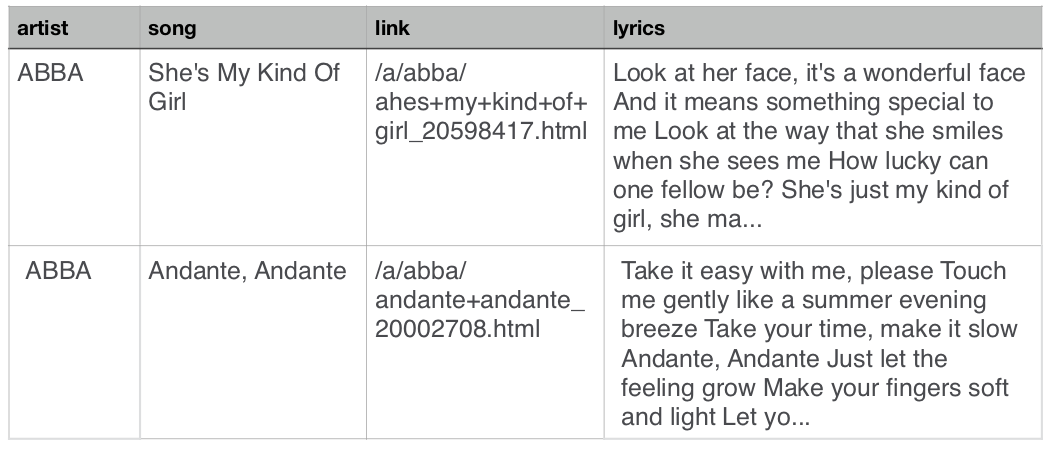
\includegraphics[height=60mm]{./img/dataset_preview.png}
	\caption{First two entries of the 55000+ Lyrics Dataset}
	\label{fig:lyrics_dataset}
\end{figure}

\subsection{User-information dataset}
To evaluate text and audio based methods on real-life user data, we had to select a dataset containing song information and lyrics as well as a dataset with information about users and their played tracks. First we tried to match the lyrics dataset onto the \textit{Echo Nest Taste Profile subset} from the Million Song Dataset website. However we only had 6800 songs with lyrics as well as user data.  We then tried the \textit{Thisismyjam} dataset also available on MSD. After removing songs we did not have lyrics for, we ended up with 16594 unique songs, and 45054 unique users. For each of the 16594 songs we also acquired a mono .wav file. \todo[inline]{Tady nevim, jestli mam rikat, ze jsem to stahla z YouTube, jestli je to jako v pohode}. \\

\section{Final dataset statistics}
Overall our final dataset had 160454 entries containing a user id, the artist, the song title and the lyrics. As our evaluation method is based on the users playlists (we took a portion of their played songs and tried to calculate the missing ones based on our metrics - will be described in more detail in the \textit{Experiment section}) we studied the dataset and especially the playlist length in more detail. //
Here are some important remarks:
\begin{itemize}
    \item Each user only has one playlist.
    \item We do not know, how many times a user played a song.
    \item We do not know which songs the user has played most recently.
    \item Users with only one song are useless for our evaluation.
    \item It should be easier to complete the dataset for users with longer datasets.
\end{itemize} 
When analyzing our dataset, it turned out, that out of 45054 users or lets say playlists, there are 22257 with only one song, which leaves us with 22797 we can use. Meaning, more than half of the playlists (about 51\% is useful for our evaluation as shown in figure \ref{fig:useless_users}.

The distribution of useful playlist lengths is shown in more detail in Figure \ref{fig:playlist_lenght_distribution}. We can see that most of the playlists are short, almost a third of them only contains two songs. The average number of songs per playlists (including those containing only one song) is 3.56. 
\begin{figure}[ht]
    \centering
	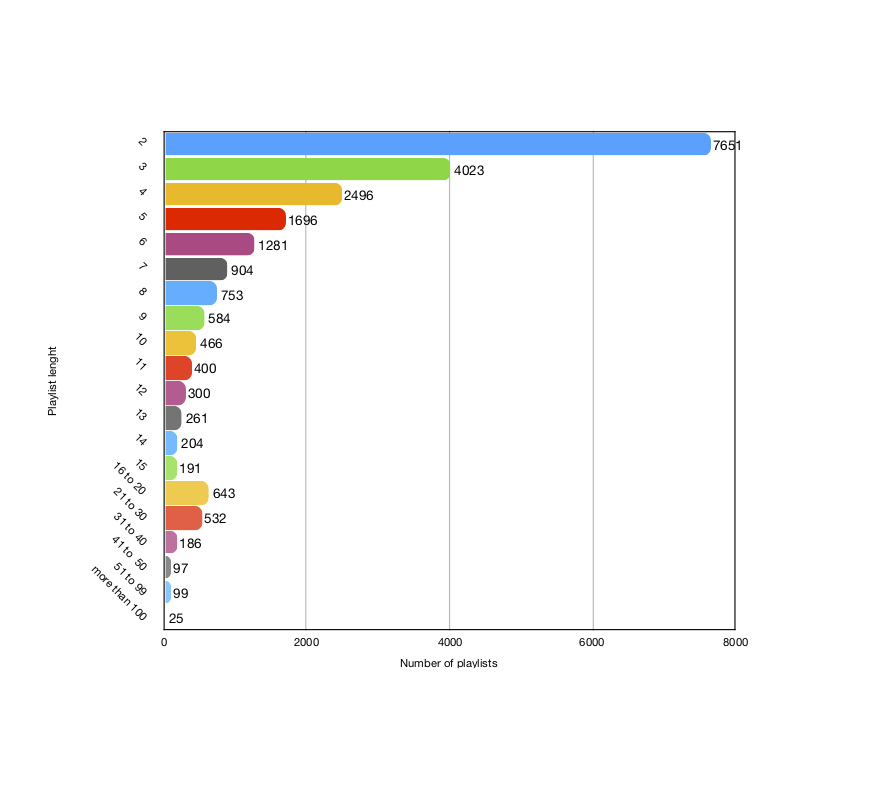
\includegraphics[height=110mm]{./img/playlist_description.png}
	\caption{The number of playlists for different lenghts}
	\label{fig:playlist_lenght_distribution}
\end{figure}
\todo{Tady mi to o 5 pisnicek nevychazi, takze to budu muset prepocitat, spis co rikate na tenhle graf? Pripadne jeste neco byste sem dodal?}

Each song has been played by 10.84 users on average. The distribution and the most popular songs are depicted in Figure \ref{fig:popular_song_distribution}. The by far most popular song with a total of 816 plays was \textit{Royals} by \textit{Lorde}. Second came \textit{Radioactive} by \textit{Imagine Dragons} with 674 users who played it. All other songs have been played by less than 500 users.

\begin{figure}[ht]
    \centering
	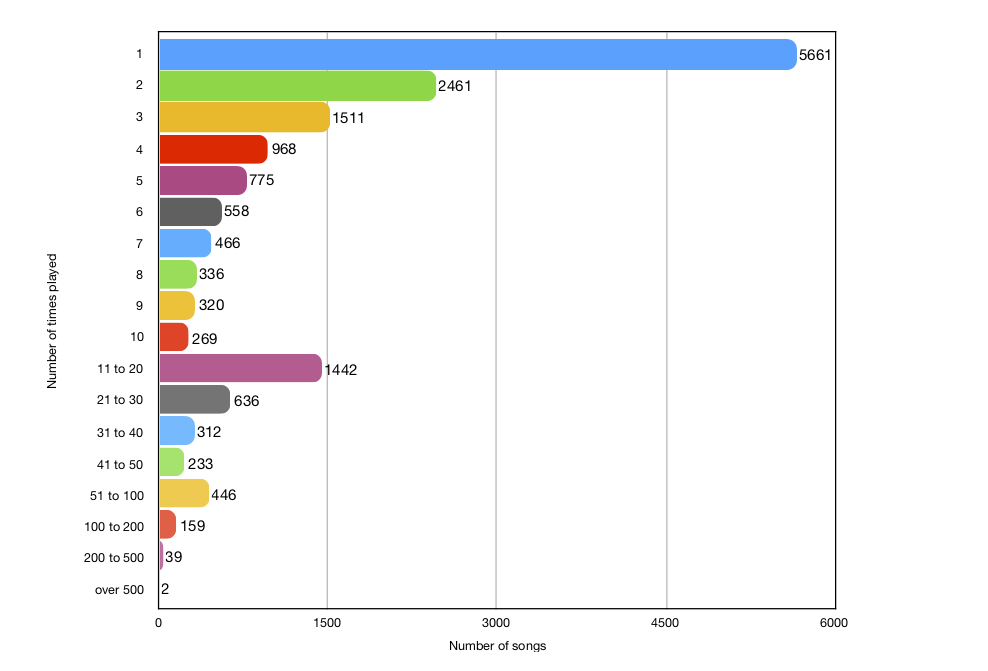
\includegraphics[height=80mm]{./img/popular_song_distribution.png}
	\caption{The number of playlists a song was in}
	\label{fig:popular_song_distribution}
\end{figure}

\chapter{Lyrics-based methods}\label{chap:lyrics_methods}
 In this chapter we will briefly describe some of the most prominent methods to represent songs based on their lyrics. After specifically focusing on the positive and negative aspects of these methods, we will select suitable candidates for testing and for our web application. The reason to explore lyrics-based methods in this thesis is based on several factors. It is the belief of the authors that although the utilization of song lyrics is not completely unexplored as shown in Section \ref{sec:text_related_work}, there is a space for innovative research. For example, to the best of our knowledge, there are no recommendation system that would rely solely on lyrics analysis. An advantage of these methods could also lie in the variety of recommendations, that would still be relevant.

\section{Text embedding methods}
\subsection{Bag of Words}
The Bag of Words commonly referred to as BoW is a text representation which counts how many times a word appears in a document. In the context of this thesis it counts how many times a word appears in the song lyrics.
Every song would be represented as a word-count vector where each index corresponds to the number of times a certain word appeared in the song. BoW is a basic representation and there are drawbacks to this approach. It for example ignores the fact that some words which can be found in most documents and have a smaller informative value than others that appear in a small fraction of documents. 
\subsection{TF-IDF}
Term Frequency-Inverse Document Frequency is another way of transforming documents into vectors. Unlike the BoW, TF-IDF does not measure only the number of words in a document but it also measures their relevance. As can be deduced from the title term frequency, first the number of appearances of a word in each document proportional to the number of all words in that document - \textit{tf} - is computed. Then comes the inverse document frequency part - \textit{idf} - where the words are weighted as seen in (3.1). The words that appear frequently in all documents have lower weights and those who only appear in some have higher weights.

\begin{equation}
idf(t) = log\frac{1+n_d}{1+df(t)} + 1
\end{equation}

Formula \ref{eq:tf_idf} is then the final Tf-idf formula multiplying the word frequencies with their weights:

\begin{equation}\label{eq:tf_idf}
tf\textnormal{-}idf(t,d) = idf(t)*tf(t,d) 
\end{equation}

where \textit{t} is the word \textit{d} is the document $ df(t) $ is the number of documents containing the word \textit{t} and \textit{n\textsubscript{d}} is the total number of documents. 

\subsection{Word2Vec}
Word2Vec is a two-layer neural network trained to encode the linguistic context of a word introduced by Tomas Mikolov in \cite{DBLP:journals/corr/abs-1301-3781}. Each word has an assigned vector in a vector space of typically hundreds of dimensions generated from a large corpus. The position of a word corresponds to its context, meaning, that words that share common context are closer to each other. \\
There are two possible Word2Vec architectures, the continuous bag-of-words and the continuous skip gram. The CBOW predicts the current word from the words surrounding it which is the context. It does not keep the order of the surrounding context words.The skip gram does, which makes it slower but also more effective, especially for infrequent words \cite{DBLP:journals/corr/abs-1301-3781}. The Skip-Gram architecture takes one word and predicts all the context around it.
\begin{figure}[h]
    \centering
	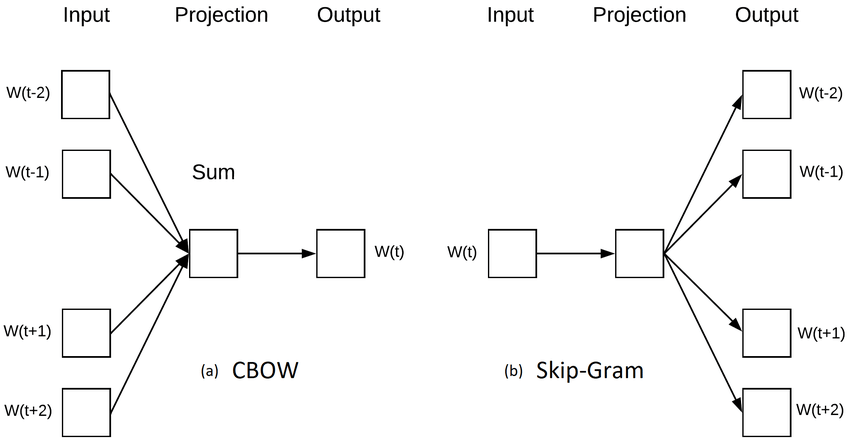
\includegraphics[height=70mm]{./img/cbow_skipgram_w2v_architecture.png}
	\caption{The CBOW and Skip-gram Word2Vec architectures from \cite{phdthesis}}
	\label{fig:cbow_skipgram_w2v_architecture}
\end{figure}
\\
Multiple things have to be taken into account when training a W2V model. The information value of words that occur in all training documents is quite low so they can be removed to increase training speed. The dimensionality of the space also elevates accuracy only to a certain point so some threshold has to be set. Another parameter is the context window, which determines, how many words before and after a given word are included as its context.

\subsection{Doc2Vec}
Doc2Vec as is an unsupervised algorithm that learns the feature representation of texts with various lengths and encodes them into vectors of the same length. As the name suggests it is heavily based on the idea of Word2Vec. It was also first presented by the same group of researches in this paper \cite{DBLP:journals/corr/LeM14}. The main idea of the method is to use the Word2Vec model but add one more vector to represent the paragraph as a whole. As in the Word2Vec model, there are two architectures for the Doc2Vec approach. The Distributed Memory (DM) version of Paragraph vector and the Distributed Bag of Words (DBOW) version of the Paragraph vector. Again, the DBOW is faster but does not consider the order of the words as it predicts a random group of words from the paragraph vector. The DM on the other hand takes previous words and the paragraph vector into account and predicts just one word. This way, because the paragraph does not shift across the text, the DM architecture is able to capture some word order.
\begin{figure}[h]
    \centering
	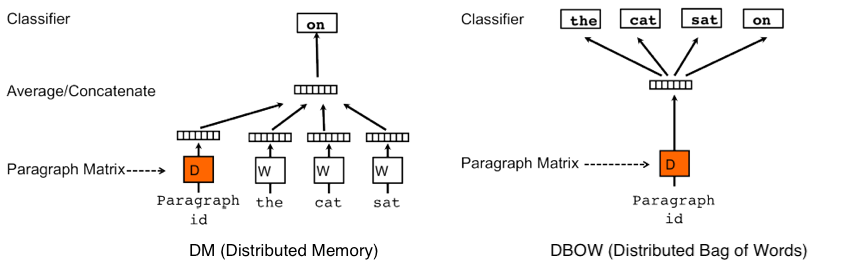
\includegraphics[width=140mm]{./img/DV_DBOW_doc2vec_architectures.png}
	\caption{The Doc2Vec DM and DBOW architecture taken from \cite{DBLP:journals/corr/LeM14}}
	\label{fig:dbow_dm_d2v_architecture}
\end{figure}
\subsection{Self organizing maps}
Self organizing maps (SOM) is a type of a neural network that learns how to reduce the dimension of input data in an unsupervised manner. SOMs were introduced by Teuvo Kohonen \cite{Kohonen1982}. They use competitive dimensionality reduction (meaning the nodes in the SOM network compete to get the right to respond to the input data) which is quite unusual for neural networks as they usually use backpropagation. The models that SOMs compute are (usually) two dimensional spaces of neurons (called \textit{codebook} vectors) where similar examples are close to each other and dissimilar examples further from each other.\\
The SOM network is trained through an iterative process. It chooses one sample \textbf{x} \( \in R^n \) from the input training set at random and teaches it to itself. During teaching, the network feeds the chosen sample into all its units. A winner unit is calculated based on a similarity measure (usually Euclidean distance) between \textbf{x} and the \textit{codebook} vectors. Finally the values of the network units are updated. The best-matching unit is moved a closer to \textbf{x} and so are all the topological neighbours of the best unit.\\
The neighbours are defined by a neighbourhood function. It decreases with time and decides how radical the change around the winner will be. There are multiple functions that can be used. One can use the Gaussian kernel around the winner, however this is quite computationally expensive. A good and more efficient function is sometimes called the \textit{"bubble"} function which is constant over the whole neighbourhood of the winner and zero elsewhere \cite{SOM_training}.
\begin{figure}[h]
    \centering
	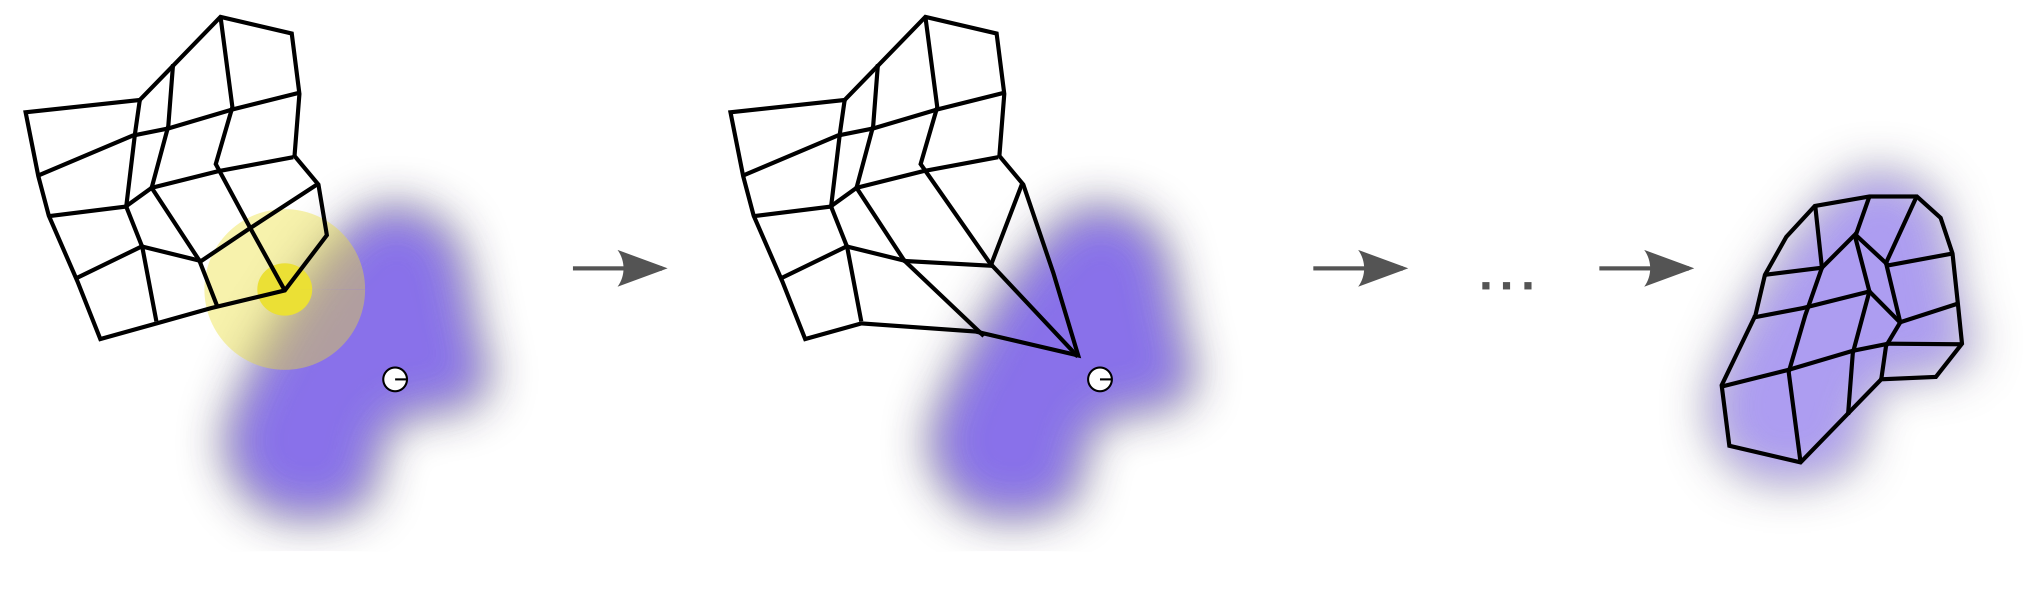
\includegraphics[width=140mm]{./img/Somtraining.png}
	\caption{Visualization of the training algorithm used for SOM networks. The blue area represents the distribution of the data. The white dot is the randomly selected sample. On the left, the SOM network nodes (units) are randomly spread accross the space. When finding a winner (middle) and its defined neighbourhood (the yellow area) the network moves towards the datapoint and eventually after repeated iterations spreads mimicking the distribution of the data (left). This image is taken from https://commons.wikimedia.org/wiki/File:Somtraining.svg}
	\label{fig:som_training}
\end{figure}



\section{Related work}\label{sec:text_related_work}
 There are several papers and on music recommendation based on lyrics. For example \cite{Gossi2016LyricBasedMR} has shown, that simple TF-IDF song embedding was 12.6 times more accurate then just random suggestions on the musiXmatch dataset \footnote{https://labrosa.ee.columbia.edu/millionsong/musixmatch}.  In \cite{inproceedings} the authors compared the Doc2Vec and SOM algorithm with cosine similarity on a dataset containing Hindi songs and found that the SOM outperforms Doc2Vec. The paper \cite{DBLP:journals/corr/Tsaptsinos17} even studies using intact lyrics as input for Recurrent (LSTM) and Hierarchical neural networks and evaluates it genre classification.
 
\section{Text representation choices}
When choosing methods for our web application there are several factors to consider. Besides the expected accuracy of the algorithms, which however is often difficult to guess as the abilities to recommend songs based on lyrics have not been researched extensively, we have to consider the implementation as well as temporal complexity features of all the methods. Also, the fact that we want to focus more on a cross-sectional approach rather than a thorough optimization of one particular algorithm, means we will prefer diversity in our chosen algorithms. \\

The Bag of Words representation could be a good choice to get some kind of baseline results. Nevertheless, since the TF-idf algorithm is widely based on the BOW and is still quite simple, we choose \textbf{TF-idf} as our baseline. As mentioned at the beginning of this chapter, it was shown to be 12.6 times more accurate on the musiXmatch Dataset (MXD) \footnote{https://labrosa.ee.columbia.edu/millionsong/musixmatch} than just random suggestions, and that is what we hope to achieve with all of our text methods. A downside of the TF-idf method is the length of its vectors. Even though they consist mostly of zeros, for our dataset, the length of each of them is over 40,000. \\
Word2Vec and Doc2Vec are two similar approaches. The issue with Word2Vec when representing a whole document, in our case lyrics for one song, is the transition between the word vectors and the whole text. A commonly used aggregation method is to define the document vector as the mean of all the word vectors. \\ 
Doc2Vec does not have this problem, as its default is suited to represent a complete text. However, the problem with Doc2Vec is the amount of data it needs for training. Because every document is one sample, the number of documents necessary to achieve reasonable results is much higher than for Word2Vec where one sample is one word. What is also convenient with Word2Vec is, that there already exists a pre-trained Word2Vec model from Google \footnote{https://code.google.com/archive/p/word2vec/}. It consists of 3 million words with a 300-dimensional vector for each. Three hundred dimensions is a reasonable number (especially considering the fact that our TF-idf vectors have over 40,000 dimensions). It was trained on roughly a billion words from a Google News dataset. Therefore we chose the Word2Vec model over the Doc2Vec. This decision was also based on a study \cite{inproceedings} showing, that Self organizing maps performed better than a Doc2Vec-based algorithm. \\
The choice of \textbf{Word2Vec} was also justified by the lack of recommendation algorithms based on it. We also decided to implement the \textbf{SOM} network rather than Doc2Vec to represent our songs as it appeared to perform well in the previously mentioned paper. It is also a bit of a more advanced way to reduce data dimensionality and it does not need as much data as the Doc2Vec to be trained. \\
One more thing we had to deal with when choosing SOM was what initial song representation to choose as input for the SOM network to be reduced in dimension. We decided to try the W2V representation. Mainly because the training of a self organizing map is quite computationally expensive and having vectors with over 40 000 dimensions would make it extremely time-consuming. We did not give up on the Tf-idf representation, we however used Tf-idf vectors pre-processed by PCA which were reduced to length 4,457. 

\chapter{Audio-based methods}\label{chap:audio_methods}
In this section we will describe the possibilities of how to transform an audio signal (in our case from a .wav file) into representations suitable for song similarity calculations. This process consists of many steps and a lot of research has been done on all of them as illustrated in Section \ref{sec:audio_related_work}. \\
The reason we are focusing on audio in this thesis is the notion, that what people care about in a song is its sound. There are patterns in music that are pleasant to the human auditory system, otherwise, music would not be so popular. We believe it is the sound wave that contains these patterns. It is difficult to define what exactly they are so we hope that with the use of unsupervised machine learning algorithms, we will be able to find these them and then locate them in unseen songs as well. \\

Figure \ref{fig:audio_extraction} illustrates the steps of audio extraction. The blue part of the diagram describes the steps that are taken to acquire various basic music representations which are explained in Section \ref{sec:basic_music_representation_methods}. Each of these representations can be given as input to a machine learning algorithm as depicted in green from Section \ref{sec:audio_machine_learning} or deep learning algorithm from Section \ref{sec:audio_deep_learning} depicted in purple which both yield a final vector representation of the song. \\

\begin{figure}[h!]
    \centering
	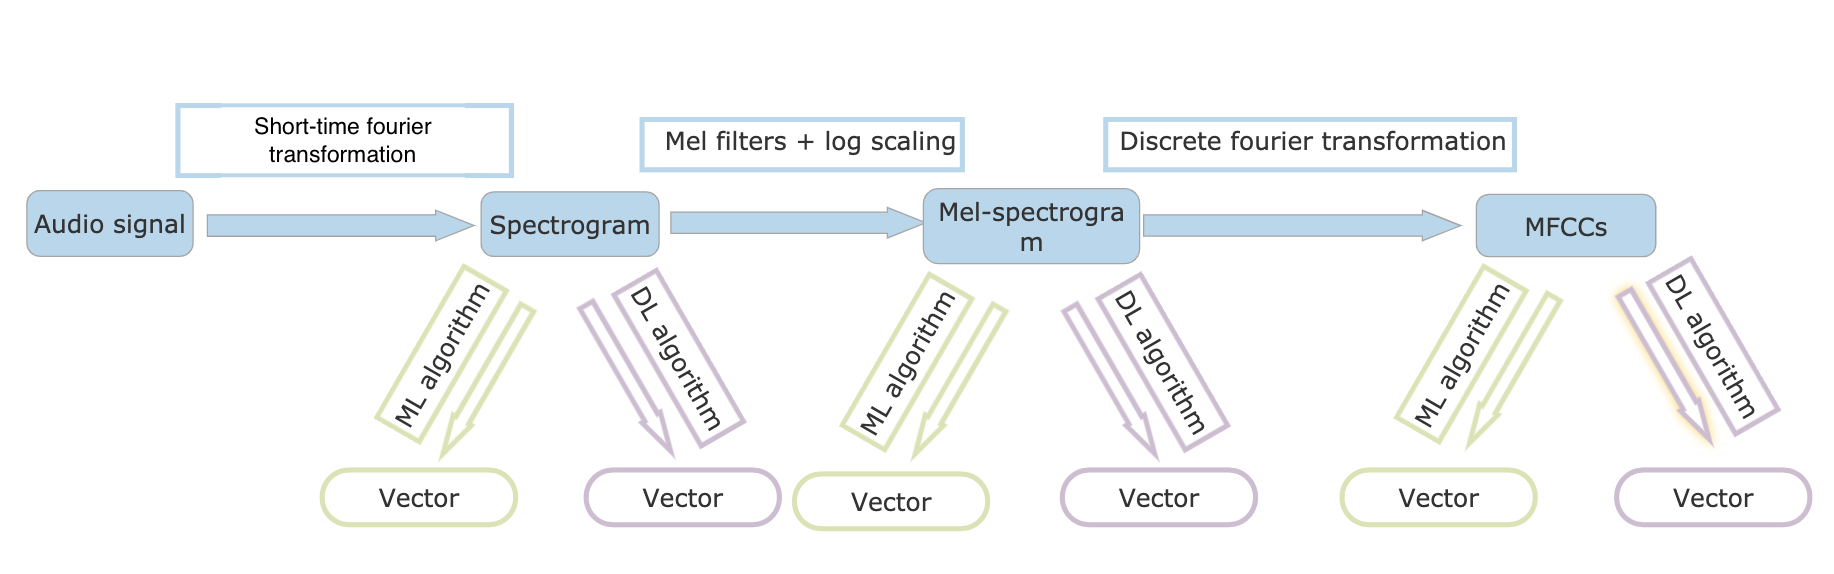
\includegraphics[width=140mm]{./img/audio_feature_extraction_steps.png}
	\caption{A diagram displaying the steps taken in audio extraction. ML stands for machine learning and DL for deep learning.}
	\label{fig:audio_extraction}
\end{figure}

\section{Basic audio representation methods}\label{sec:basic_music_representation_methods}
 

\subsection{Raw waveform}
Sound is as vibration that spreads through gas, liquid or solid as a wave of pressure. For humans, the sound we hear has a frequency between 20Hz and 20kHz. Other sound waves are inaudible for humans. The most basic representation of sound as an audio signal is a \textit{waveform}. It captures the variation of pressure over time. As we cannot store infinite data to capture the state of the wave in every moment, we need to establish a sample rate. The sample rate is the number of samples per second at which the pressure is recorded as amplitude. Common sample rates are 44,100 Hz and 22,050 Hz that capture oscillation up to 22,050 Hz and 11,025Hz \cite{Schluter2017}.

\subsection{Spectrograms}
Raw waveform data have a lot of data points which makes them spaciously demanding. Luckily, they also display strong regularities in their oscillations which gives us a different, more compact possibility to represent audio signal. It encodes the signal as the strength of oscillations at various frequencies as opposed to amplitudes over time. Such an encoding is called a \textit{spectrum} when sinusoids are used as prototypical oscillations.
The spectrum is obtained from a waveform by applying \textit{Discrete Fourier Transformation}. The signal after DFT is represented by oscillations of a few frequencies spanning the full signal. \\
However a problem with this approach is, that for longer recordings, many oscillations are present only over some limited time span or change frequency. To represent all the oscillations the \textit{Short-Time Fourier Transformation} can be computed. It slices the audio into small often overlapping windows, computes their spectra and then puts them together in a chronological order. This spectra matrix is called the \textit{spectrogram} and for the song 'Someone Like You' by 'Adele' it has the shape of (2206, 7796). It can be visualized as a graph with frequency on one axis and time on the other axis. The intensity of a frequency is represented by color.

\begin{figure}[h!]
    \centering
	\includegraphics[width=140mm]{./img/spectrogram.png}
	\caption{Spectrogram of the song 'Someone Like You' by 'Adele'. The intensity of different frequencies over time is converted to decibels.}
	\label{fig:ilustrative_specrogram}
\end{figure}


\subsection{Mel Spectrograms}\label{ssec:mel_spectrograms_intro}
Mel-spectrograms are another approach to reducing the dimensionality of our data. However they are not mathematically based reductions of any kind of feature space. They are filtered spectrograms. Frequency bands are extracted by applying triangular \textit{Mel scale} filters to the power spectrum. The \textit{mel scale} after which this the spectrograms are called was named in 1937 in a study \cite{1937ASAJ....8..185S} by Volkmann and Newman. Since then it has been re-formulated multiple times, for example in \cite{mel_scale_fit} by Umesh at al. It is based on the human perception of pitch and loudness and allows us to convert from Hz to Mels. Mels which are more discriminatory at lower frequencies and less at higher frequencies - as is the human ear. \\
Each of the triangular filters has a response going from 1 to 0. They respond 1 at the center of some frequency and then their response decreases linearly to 0 towards to the place where they meet the neighbouring filters. When these filters are applied to a spectrogram, we get a mel-spectrogram. It is again a matrix of a smaller shape this time (320, 7796) for 'Someone Like You' and it can also be visualized as illustrated in Figure \ref{fig:ilustrative_melspecrogram}.

\begin{figure}[h!]
    \centering
	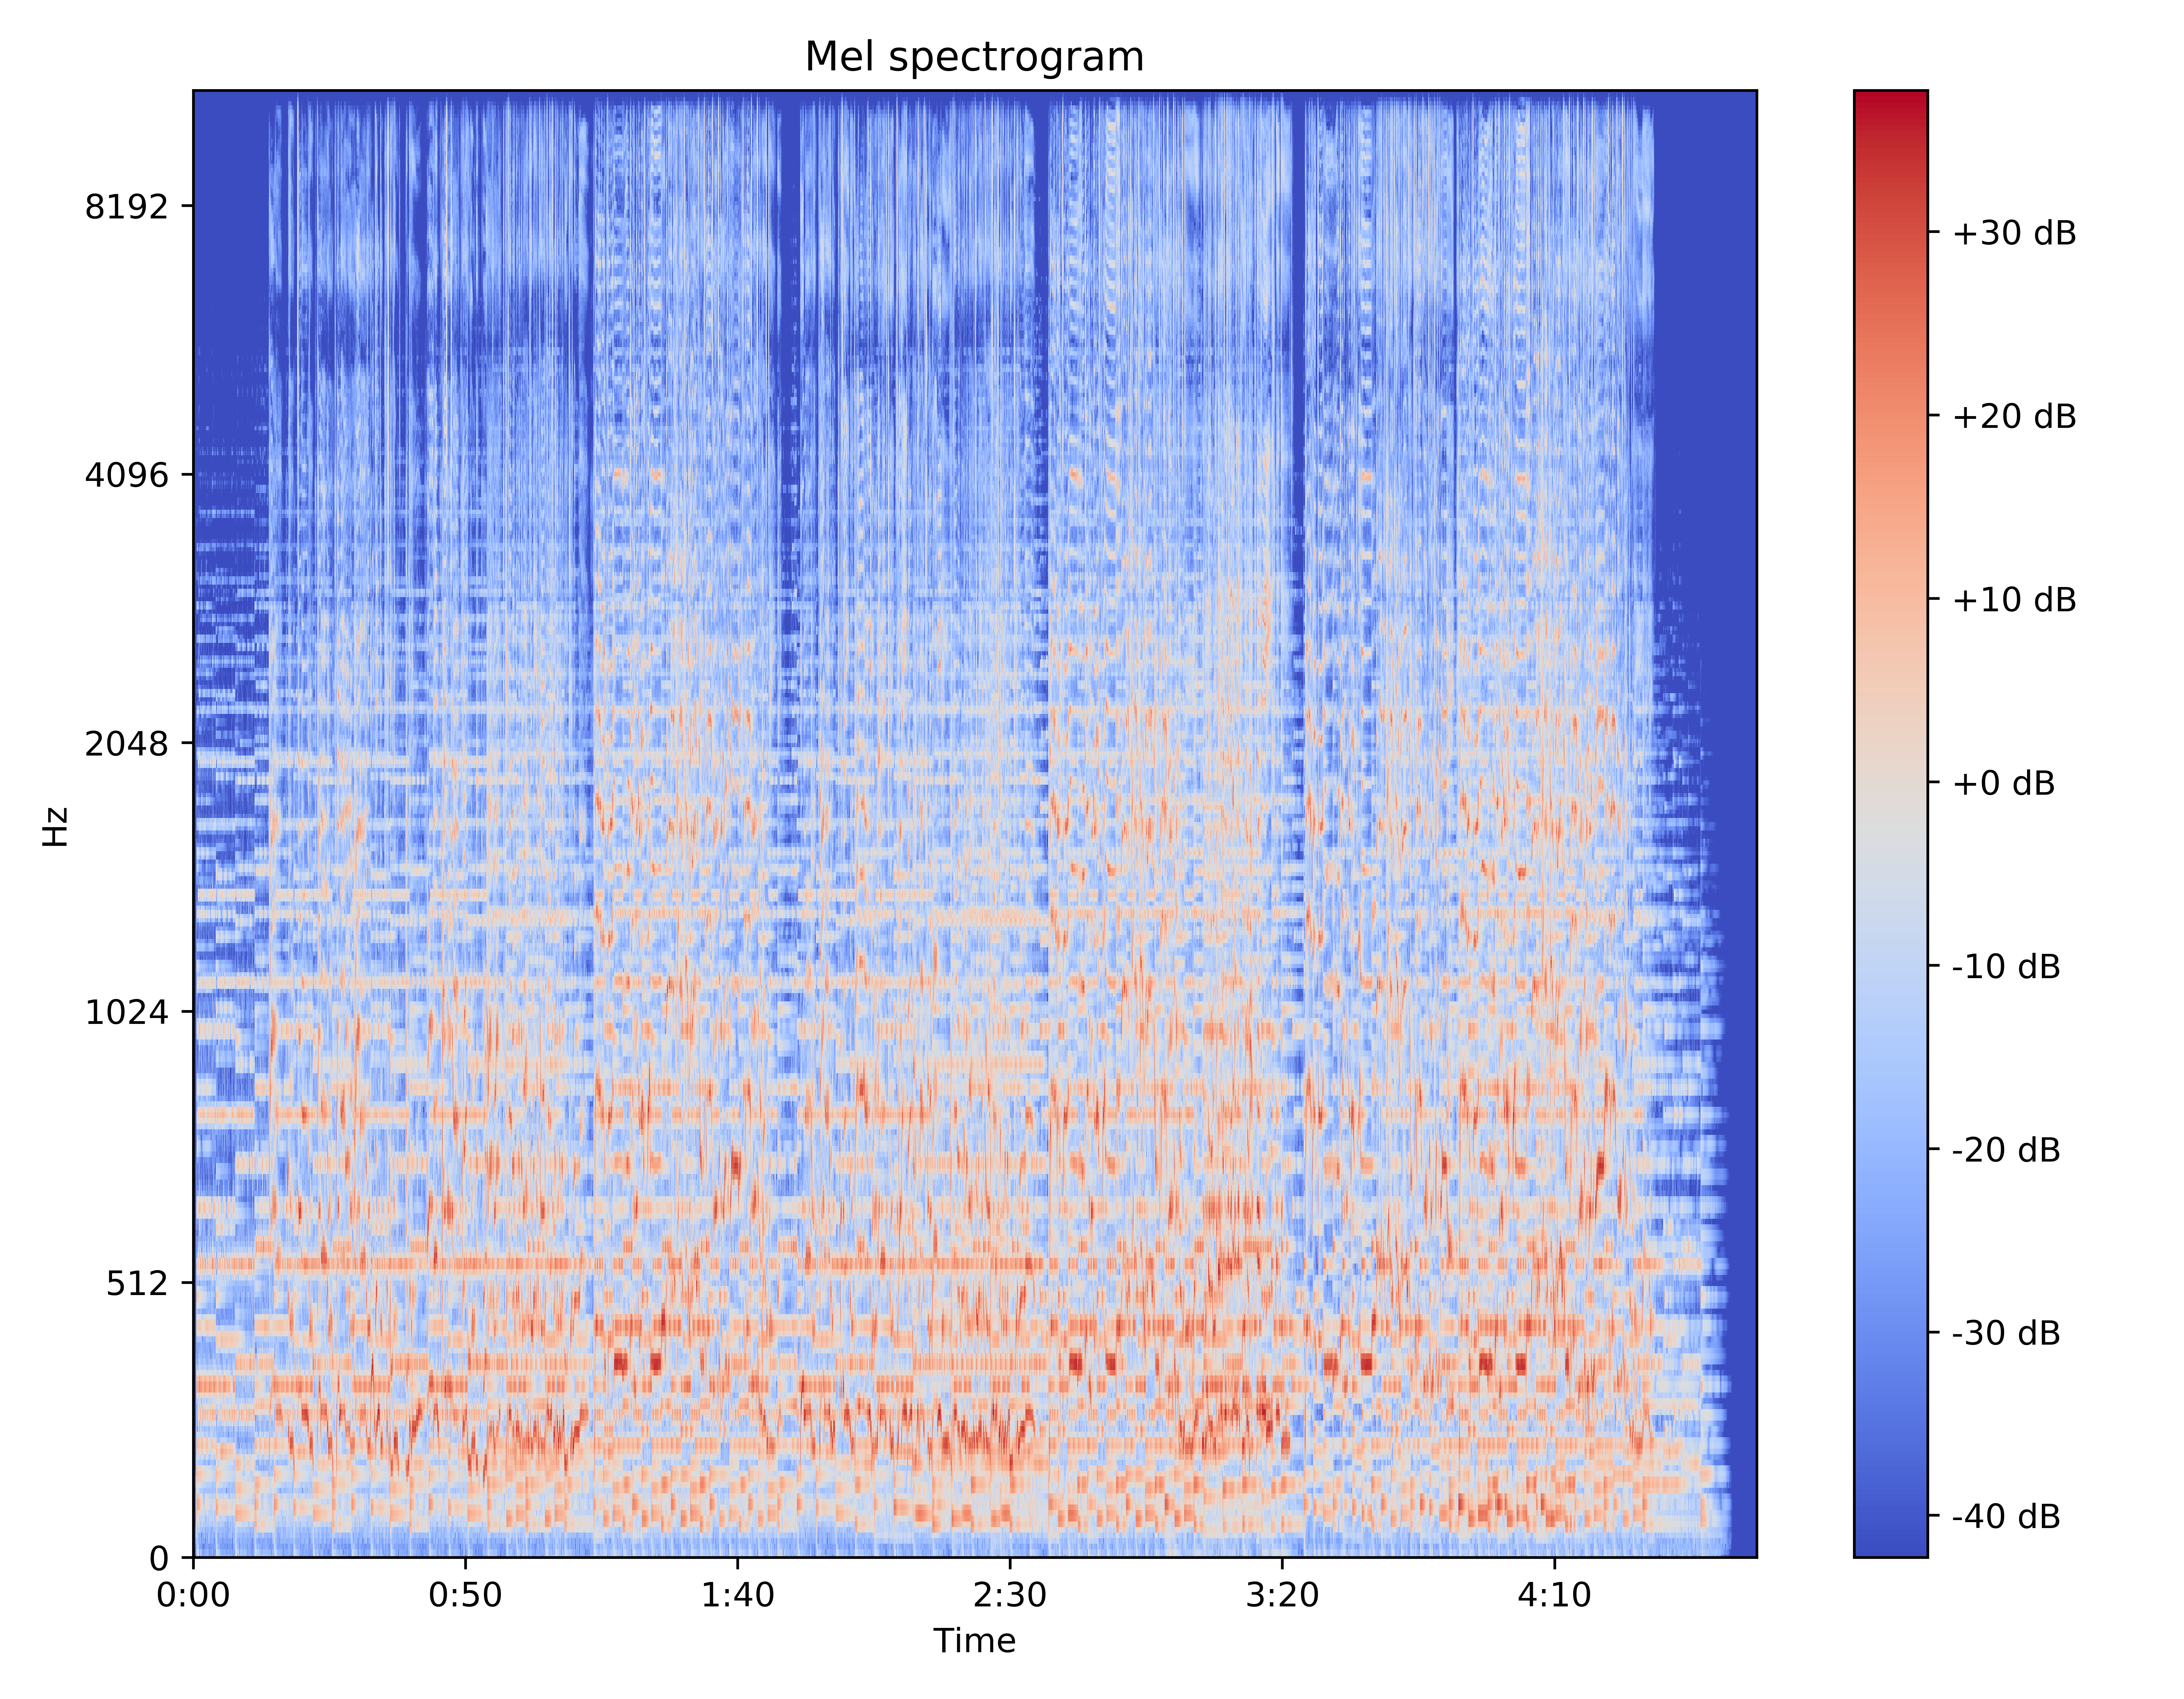
\includegraphics[width=140mm]{./img/melspectrogram.png}
	\caption{Mel-spectrogram of the song 'Someone Like You' by 'Adele'. The intensity of different frequencies over time is converted to decibels.}
	\label{fig:ilustrative_melspecrogram}
\end{figure}

\subsection{Mel Frequency Ceptral Coefficients}
Mel-Frequency Ceptral Coefficients (MFCC) are another step further in extracting audio features. They are obtained by applying \textit{Discrete cosine transformation} to mel-spectrograms. The DCT yield an even more compressed representation of them. For the song 'Someone Like You' by 'Adele' which we used as an example for spectrograms as well as mel-spectrograms, it created a matrix of shape (128, 7796) which looks as Figure \ref{fig:ilustrative_mfccs} illustrates.\\

A nice introcution to music signal processing with respect to deep machine learning, where spectrograms, mel-spectrograms and MFCCs are explained in more detail can be found here \cite{Schluter2017} where we also drew a lot of our information from.

\begin{figure}[h!]
    \centering
	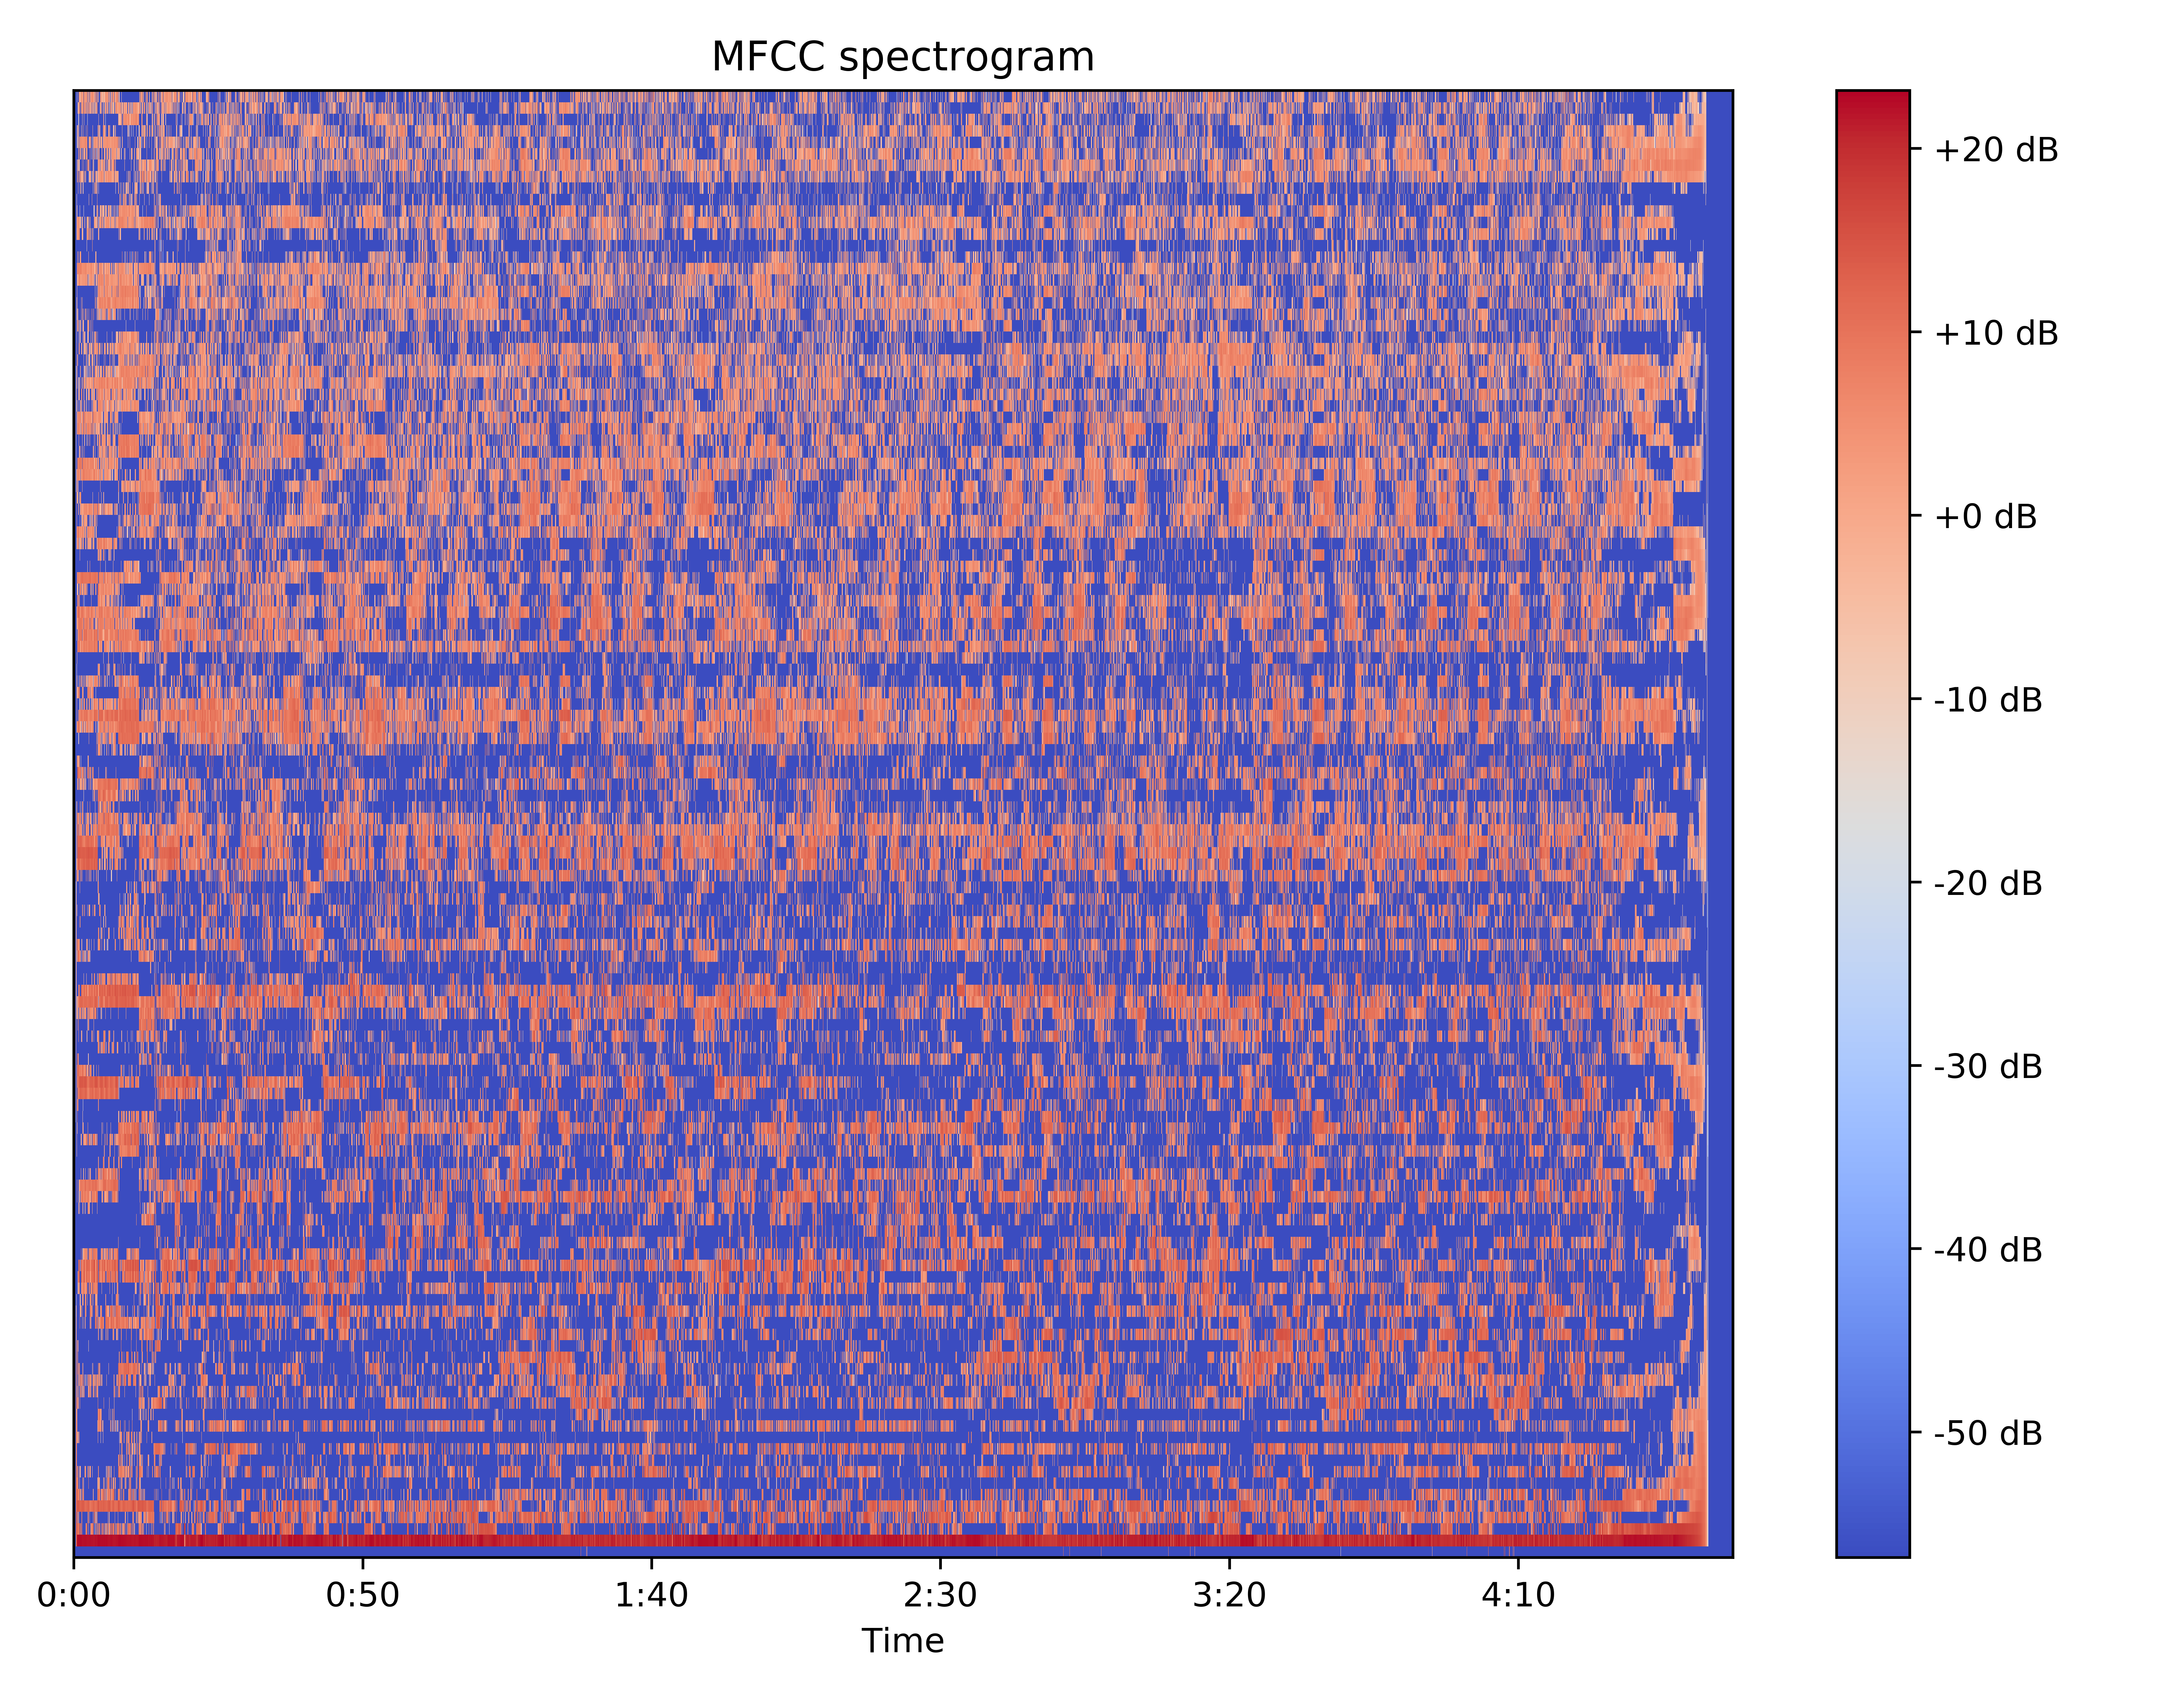
\includegraphics[width=140mm]{./img/mfccs.png}
	\caption{MFCCs of the song 'Someone Like You' by 'Adele'. The intensity of different frequencies over time is converted to decibels.}
	\label{fig:ilustrative_mfccs}
\end{figure}

\section{Simple audio representation methods}\label{sec:audio_machine_learning}

\subsection{PCA}
PCA is a common machine learning algorithm used to reduce dimensionality of the feature space. It tries to keep features with most variance and discards feature in which all the data points are highly correlated. The data space is transformed in such a way, that the first principal component (PC) has the largest possible variance, the second PC the second largest variance etc. \\
Mathematically it is a orthogonal linear transformation to a new coordinate system where the base vectors are the principal components. To achieve this, we first need to center the data around the origin. That is done by subtracting the mean of each variable from the data. After that a covariance matrix is computed with its eigenvalues and corresponding eigenvectors. After normalizing the eigenvectors, they can be interpreted as a new basis vector. This new basis transforms the covariance matrix so that it becomes diagonal. Each of the diagonal elements represents the variance of each axis. All the components without any reduction give us the whole information about the input data, only in a vector space with a different basis. Every component explains some portion of the data's variance. The variance can be calculated by dividing every eigenvalue corresponding to an eigenvector with the sum of all eigenvalues. The dimensionality reduction is dependant on how many components we want. If we want to visualize the input data in a 2D graph, we create a space with only the first two PCs as a base and map all the data onto it. The reason to use this algorithm in our thesis is be mainly to reduce the length of the audio flattened audio matrices. \\
The PCA assumes that there is linear correlation between features. If there is not, the PCA will not discover it and will loose a lot of information with the dimensionality reduction it performs.

\section{Deep audio representation methods}\label{sec:audio_deep_learning}

\subsection{Convolutional neural networks}
Convolutional neural networks are neural networks that have become extensively researched after AlexNet (a form of CNN) was demonstrated in 2012 and outperformed all other methods for visual classification \cite{Krizhevsky:2012:ICD:2999134.2999257}. As with other neural networks, CNN's biggest advantage is to emulate behavior of unknown non-linear functions. CNNs have the ability to map high-dimensional data into a space of finite categories (with hundreds or thousands of classes). They are mostly used in visual imagery tasks. \\
The idea behind convolutional neural networks is to use \textit{local filters} instead of creating fully connected layers. This has risen from the idea that in images, there are correlated compositions on short scale distances, rather than at large distances. For example when detecting a human face in an image with a tree in the background, the tree does not have much to say about the face, unlike the eyes or the nose by which the face can be identified and are in a much greater proximity to each other. This is also the reason why in the CNN's architecture, the layers are not fully connected. \\
There are 4 main components that are generally be included in every CNN network. The \textit{Convolution layer},the \textit{ReLU}, the \textit{Maxpooling layer} and the \textit{Fully connected layer} that yields the output. To briefly describe these layers lets start with convolution. The convolutional layer helps to reduce the number of connections and weights. It consists of filters that can be learned. These only take a small number of nearby features into account at a time but extend through the whole input. Each of the filters crates a 2D activation map by computing the dot product of entries of the filter and the input. ReLU (rectified linear unit) is generally used to increase non linear properties of the decision function. Its function is $ f(x) = max(0,x) $ which is applied to the results of the convolution to speed up training --- compared to previously used functions for example sigmoid functions --- without affecting the receptive fields of the convolution layer. The pooling layer also reduces the number of parameters and helps prevent over-fitting. The most common function to implement is \textit{max pooling}. The features are partitioned into a set of non-overlapping rectangles (if input is 2D) and each of these rectangles  is represented by its maximal value. 
The final layer is usually a fully connected. Its neurons have connections to all activations of the previous layer and their activation is then computed as an affine transformation. 

\subsection{Deep belief networks}
Deep belief networks introduced by Hinton \cite{Hinton504} are multiple \textit{Restricted Boltzmann machines} greedily stacked on top of each other. RBMs are shallow two-layer neural nets created by Paul Smolensky in 1986 \cite{Smolensky1986InformationPI}. The first layes is called the visible layer, the second layer is called the hidden layer. The nodes of each layer communicate with the previous and subsequent layer but there are no connections between nodes of the same layer. Each visible node takes a low level feature to be learned and multiplies it by some weight. The results for each feature of an input sample are then summed, bias is added and this is the result passed through and activation algorithm which produces an output for each hidden node. These outputs then can be redirected into another hidden layer instead of the output of the neural network. \\
RBMs also have the ability to reconstruct data without supervision. When the input makes it through both layers it then becomes input for the hidden layer and travels through the neural network in the opposite direction. The activations are multiplied by the same weights and passed to the visible layer where a new bias is added. The output of the visible layer is then compared to the initial input and the network adjusts weights so that it minimizes the difference between the input and the output.

\subsection{Recurrent neural networks}
Recurrent neural networks have one major difference compared to other neural networks. They include feedback loops in their structure which allows them to exhibit dynamic behaviour and makes them useful for processing sequential data. RNNs have a hidden state that is determined by previous states and is updated with every subsequent step. There are many variants of RNNs such as \textit{Fully recurrent, Long short-term memory} introduced by Hochreiter and Schmidhuber in \cite{doi:10.1162/neco.1997.9.8.1735}, \textit{Gated recurent units} first described in \cite{cho-etal-2014-learning}, or \textit{Bi-directional} invented by Schuster and Paliwal in \cite{Schuster1997BidirectionalRN}. \\
Recurrent neural networks are used for working with sequential data for example in speech recognition \cite{DBLP:journals/corr/abs-1303-5778} or time-series anomaly detection \cite{inproceedings_RNN_anomaly_detection}.


\subsection{Autoencoders}
Autoencoders are not tied to one type of neural network. They can be build from recurrent layers, convolutional layers or using a simple Multi-layer Perceptron.\\
The autoencoder has two parts the encoder and the decoder. It is trained in an unsupervised manner. The encoder takes the input data and reduces its dimensions. The decoder then tries to recreate it into its original form without knowing, what the data looked like before the encoder processed it. The idea is, that over time, the encoder learns how to shrink the data with retaining as much information as possible for the decoder so the decoder it is able to recreate the original form as accurately as possible. 

\section{Related work}\label{sec:audio_related_work}
For the signal representation, there is obviously the possibility to use raw audio data as input for any machine learning algorithm. This however is a quite uncommon approach and when tested recently in tag prediction \cite{6854950} it had worse results than standard spectrograms. Multiple studies and experiments have been done using spectrograms as audio representation for classification tasks --- for example \cite{wang2014improving} --- or for unsupervised learning \cite{van2013deep}, \cite{Ramakrishnan2017song2V}, \cite{NIPS2009_3674}, which is what also our area of interest. \\
In these studies the inputs were fed into various neural network. The output of those was then evaluated and compared to music classification or simply music similarity estimation using similarity measures directly on spectrograms. We are going to do a similar thing in this thesis. Our evaluation will be done on user playlists and the methods will be compared to each other.

\section{Audio implementation choices}

\subsection{Basic audio representation choices}
At first when developing the web application we had the hope of using at least some of the raw data representation, to build some sort of base-line model. However, this turned out to be quite difficult as the vectors from flattened spectrograms, mel-spectrograms and mfccs have tens sometimes even hundreds of thousands of features. Therefore, although we implemented and evaluated recommendations based on mel spectrograms and mfccs, to include them in the proposed web application turned out to be too time consuming. The specific reasons are described in more detail in Chapter \ref{chap:experiments}. For the application, only PCA transformed mel-spectrograms and MFCCs were selected as they have a significantly reduced number of dimensions.


\subsection{Deep Audio representation choices}
Neural networks are a quickly developing and expanding field with many various applications. It is difficult to build an accurate neural network for specific task even with experience in deep machine learning. Because that is not what we have, we chose our neural network architecture and parameters based on literature relevant to the topic of audio-based music recommendation. The main requirements we had for our algorithms was that they have to work in an unsupervised manner and that they have to reduce the feature space. This pruned the number of possibilities for us considerably, as most architectures are designed for music classification (mostly into genres) or speech and sound recognition. \\
We decided that autoencoders suite our task in this thesis best. It is an unsupervised algorithm, with the task is to encode the input sample into a smaller dimension which is exactly what the encoder part does. The decoder transforms it again into the same vector however, this part of the autoencoder is only necessary for training.\\
Since we are working with sound data, the choice was to use RNN layers which have the ability to encode sequences (spectrograms, mel-spectrograms and mfccs are 2D matrices). These choices were mainly inspired by this paper \cite{inproceedings_RNNs}. However we want to add more methods into comparison, so we implemented not only neural networks with GRU layers but also LSTM layers and used spectrograms, mel-spectrograms and also mfccs as input rather than focusing on one type of layer, input and tuning one particular neural network to give the best results possible. 
\chapter{Experiments}

In this chapter we describe how the chosen song encoding methods were implemented. This includes describing the input, training (if there was any) and output (meaning the vector-encoded representations for each song in our 16594 songs dataset). We also acquaint the reader with our evaluation methods, the reason we decided to use them and the evaluation results for each method. The results are first presented separately for each method (or a group of closely related methods) and then summarized and most importantly interpreted in the \ref{sec:discussion} where various graphs and tables illustrating the prominent or interesting trends and tendencies can be found. Before all this however, we start with stating what the expected outcomes were before we even started.

\section{Expectations}

Even before reading any literature, we made two main predictions. 
\begin{itemize}
    \item \textbf{First:} Audio-based methods will perform better than text-based methods.
    \item \textbf{Second:} More advanced methods will outperform simpler machine learning methods.
\end{itemize}
These were based on our intuition and later also supported by reading into this topic, where most of the papers we studied were describing neural networks performing similar audio or text-based recommendation or classification and their results were compared to simpler algorithms. However, this has not proven to be accurate with our evaluation dataset. The reasons for why it might be the case are described at the end of this chapter in the \textbf{Discussion} section. \\
We were also hoping, that the text-based methods will not be complete irrelevant. In this case, we were right, but only to the extend that the text-based methods are not irrelevant in comparison to the audio-based methods. Overall, all the methods have shown that they seem to lack the properties to be useful as methods for recommendation.
\section{Evaluation}

\subsection{Wanted recommender-system features}
We already touched this in the introduction but it is useful to revise what we want from a good recommendation system and what its most important features are. Let's skip the software part for now (as it will be discussed further in the \textbf{Web application} chapter and focus purely on what it recommends. Probably the most crucial property a recommendation system should have is that it should include the items the user actually likes between the first 10 to maybe 50 recommendations. Because it does not really matter if an item the user would like ends up on the 500th or 5000th position. People rarely go that deep. \\
Another thing we would want is for the system to be able to improve its recommendations with a rising amount of data it acquires about a user. In our case this means, that we would expect the predictions to be better for users with longer playlists. \\
Even though the whole idea of this thesis is to approach recommendation more loosely, we still want our methods to posses these features to at least some reasonable extend. Also, as these are the properties other recommendation systems are being evaluated on, we can gain a better understanding of the features our methods share with other recommendation techniques as well as their where they differ. 
\subsection{Evaluation measures}
To test the wanted features described in the section above we performed evaluation as follows. \\
Our dataset contains 11123 playlists that were used to evaluate our algorithms. We chose to evaluate our algorithms only on playlists of length at least four. For each method, we did a 5-cross-validation where in a validation epoch, every playlists $p_i$ was divided into two parts a training part $p_{i_{train}}$ and a testing part $p_{i_{test}}$ with an approximately 80:20 ratio. A higher priority was set on the fact that the test part always had to contain at least one entry (meaning that for playlists of length 2, the ratio would be 50:50). \\
Afterwards for each song $ s_k $ from our song dataset $S$, the similarity of the whole $p_{i_{train}}$ to $s_k$ which we denote as $ sim(p_i, s_k) $ was calculated as $sim(p_i, s_k) =$ $\sum_{s_j\in{p_i{_{train}}}} cos_sim(s_i, s_j) $ where $ i \neq j$ and $cos_sim$ is the cosine similarity as defined by Python scikit-learn package. These similarities were then sorted and it was determined at what position the songs from $p_{i_{test}} $ that actually belong to the playlist came. \\
These positions were then used to calculate multiple evaluation measures used to assess how well does each algorithm predict the missing part of a users playlist. For this we chose the following for methods:
\begin{itemize}
    \item Recall at 10 (= \textbf{R@10}) defined as the number of songs from $p_{i_{test}} $ that placed in the top ten most similar songs.
    \item Recall at 50 (= \textbf{R@50}) defined as the number of songs from $p_{i_{test}} $ that placed in the top fifty most similar songs.
    \item Recall at 100 ( = \textbf{R@100} ) defined as the number of songs from $p_{i_{test}} $ that placed in the top hundred most similar songs.
    \item Normalized cumulative discounted gain (= \textbf{nCDG}) defined as 
    $${nDCG_{r}} = \frac{DCG_{r}}{IDCG{r}} $$
    where 
    $${DCG_{r}} =\sum_{i=1}^{r}{\frac {rel_{i}}{\log _{2}(i+1)}} $$ 
    is the discounted cumulative gain at position r and 
    $$ {IDCG_{r}} =\sum _{i=1}^{|REL|}{\frac {2^{rel_{i}}-1}{\log _{2}(i+1)}} $$
    is the ideal discounted cumulative gain at r
    where $r$ is in our case the number of songs that had to be predicted, the $rel_i$, meaning relevance, is the same for all songs as all songs in one playlists have the same relevance and $|REL|$ is the list of relevant items (in our case the songs from $p_{test}$).
    \item Average rank of a song from the $p_{i_{test}}$ set $ \boldsymbol{ (= \overline{rank})} $ which we included after the first four mentioned did not really meet our expectations.
    \item A graph plotting the distribution of rankings of songs from the test part of each playlists which we called the \textit{RDG} (=\textit{rank distribution graph}). We summed the number of songs from $p_test$ to which each individual rank from 1 to 16594 and divided it by the number of all songs that were in a testing part of some playlist. So for example if we had two playlists both with two songs from $p_{test}$ and our method assigned ranks 30 and 2900 to the $p_{test}$ songs from the first playlist and 2900 and 4872 to those from the second playlists, our graph would plot the values 0.25 for rank 30, 0.5 for rank 2900 and 0.25 for rank 4872 and 0 for the rest of the ranks. We did this for all playlists together but we also plotted the distributions for chosen playlist lengths separately to see if our predictions improve for longer playlists as we were hoping for. The x-scale of the \textit{RDG} was scaled logarithmicaly as we are much more interested in what is going on on the first 100 positions than what is goint on in the middle or towards the end. 
    
\end{itemize}
We calculated each of the first four measures for each playlist and then averaged over the whole playlist dataset. Every method section contains a table with the four measure averages and a graph. Both are accompanied with a short summary of the most obvious observations

To make things more easy for the rest of the thesis we introduce a nomenclature for our experimental methods. There are 3 different parts each of our method has. The name of the main algorithm, the name of the input and the length of the output vector. Every method can be uniquely identified by a combination of these three parts. Where there is only one or two of these necessary, we omit those which are surplus.\\
So for example a PCA method with spectrogram input and the output vector length of 320 is denoted as PCA\_spec\_320. If we take a look at the notation of the Tf-idf method, it will be only Tf-idf as there are no variations to it. However the PCA with Tf-idf input will be PCA\_Tf-idf. We separate the name parts with '\_' 

Just before we dive into the description of each method and it's results, 
\section{Text method experiments}

\subsection{TF-idf experiments}\label{ssec:TF_idf}


\subsubsection{Input}
The lyrics for each song were stripped of all punctuation characters as well as apostrophes, converted into a single string. 
\subsubsection{Training}
Each lyric-string was appended to the whole training dataset which was then passed to an instance of \texttt{sklearn.feature\_extraction.text.TFidfVectorizer} where the method \texttt{fit\_transform} was called. The results were saved into a numpy file containing a sparse matrix. And the model was saved using pickle.\\

\subsubsection{Output}
The song representation were vectors of length 40165 which is the number of different words our dataset contained.

\subsubsection{Results}

The results of the TF-idf method were poor overall when it comes to satisfying the properties of recommender systems.In comparison to our other methods however, they placed well above average. \\

\begin{table}[h!]
\centering
\renewcommand{\arraystretch}{1.5}
\begin{tabu} to 1\textwidth {| c || X[c] | X[c] | X[c] | X[c] | X[c] | }
 \hline
 \textbf{method} & \textbf{R@10} & \textbf{R@50} & \textbf{R@100} & \textbf{nGDC} & $ \boldsymbol{\overline{rank}} $ \\
 \hline
 \hline
 Tf-idf & 0.04293 & 0.05051 & 0.05619 & 0.03594 & 7553 \\
 \hline
 PCA on Tf-idf & 0.05091 & 0.05909 & 0.06393 & 0.04107 & 7345 \\
 \hline
\end{tabu} \\
\caption{Table summarizing average TF-idf and Tf-idf with PCA values averaged over the 5 cross validation that were performed}
\label{table:1}
\end{table}

When looking at the number in \ref{table:1} we can see that only 4.3\% of songs that were in our $p_{test}$ sets ranked in the first ten, 5\% in the first fifty and 5.6\% in the first hundred. The average rank of a song from our $p_{test}$ was 7553 which is quite close to the middle. This does not really satisfy our goals that we set to achieve in recommender systems. We also crated a \textit{RDG} as one can see in Figure \ref{fig:tf_idf_distribution}. It appears that according to the distribution, a song is more likely to end up in the first 10-100 songs than it is at the end. One could claim that this distribution is not random and favors ranks at the beginning, however not as strongly as we would want.\\
Another thing to notice in \ref{fig:tf_idf_distribution} is that there is a general trend for the Tf-idf method to perform worse on playlists with a greater length. This is the complete opposite of what we desire. One can see, that for playlists with length from 4 to 6, the ranks predicted for the missing songs were more likely to be higher than for playlists of length 21 and longer. The pink bar shows the overall distribution over 5000 bins over the dataset. 

\begin{figure}[h]
\centering
\begin{minipage}{.5\textwidth}
  \centering
  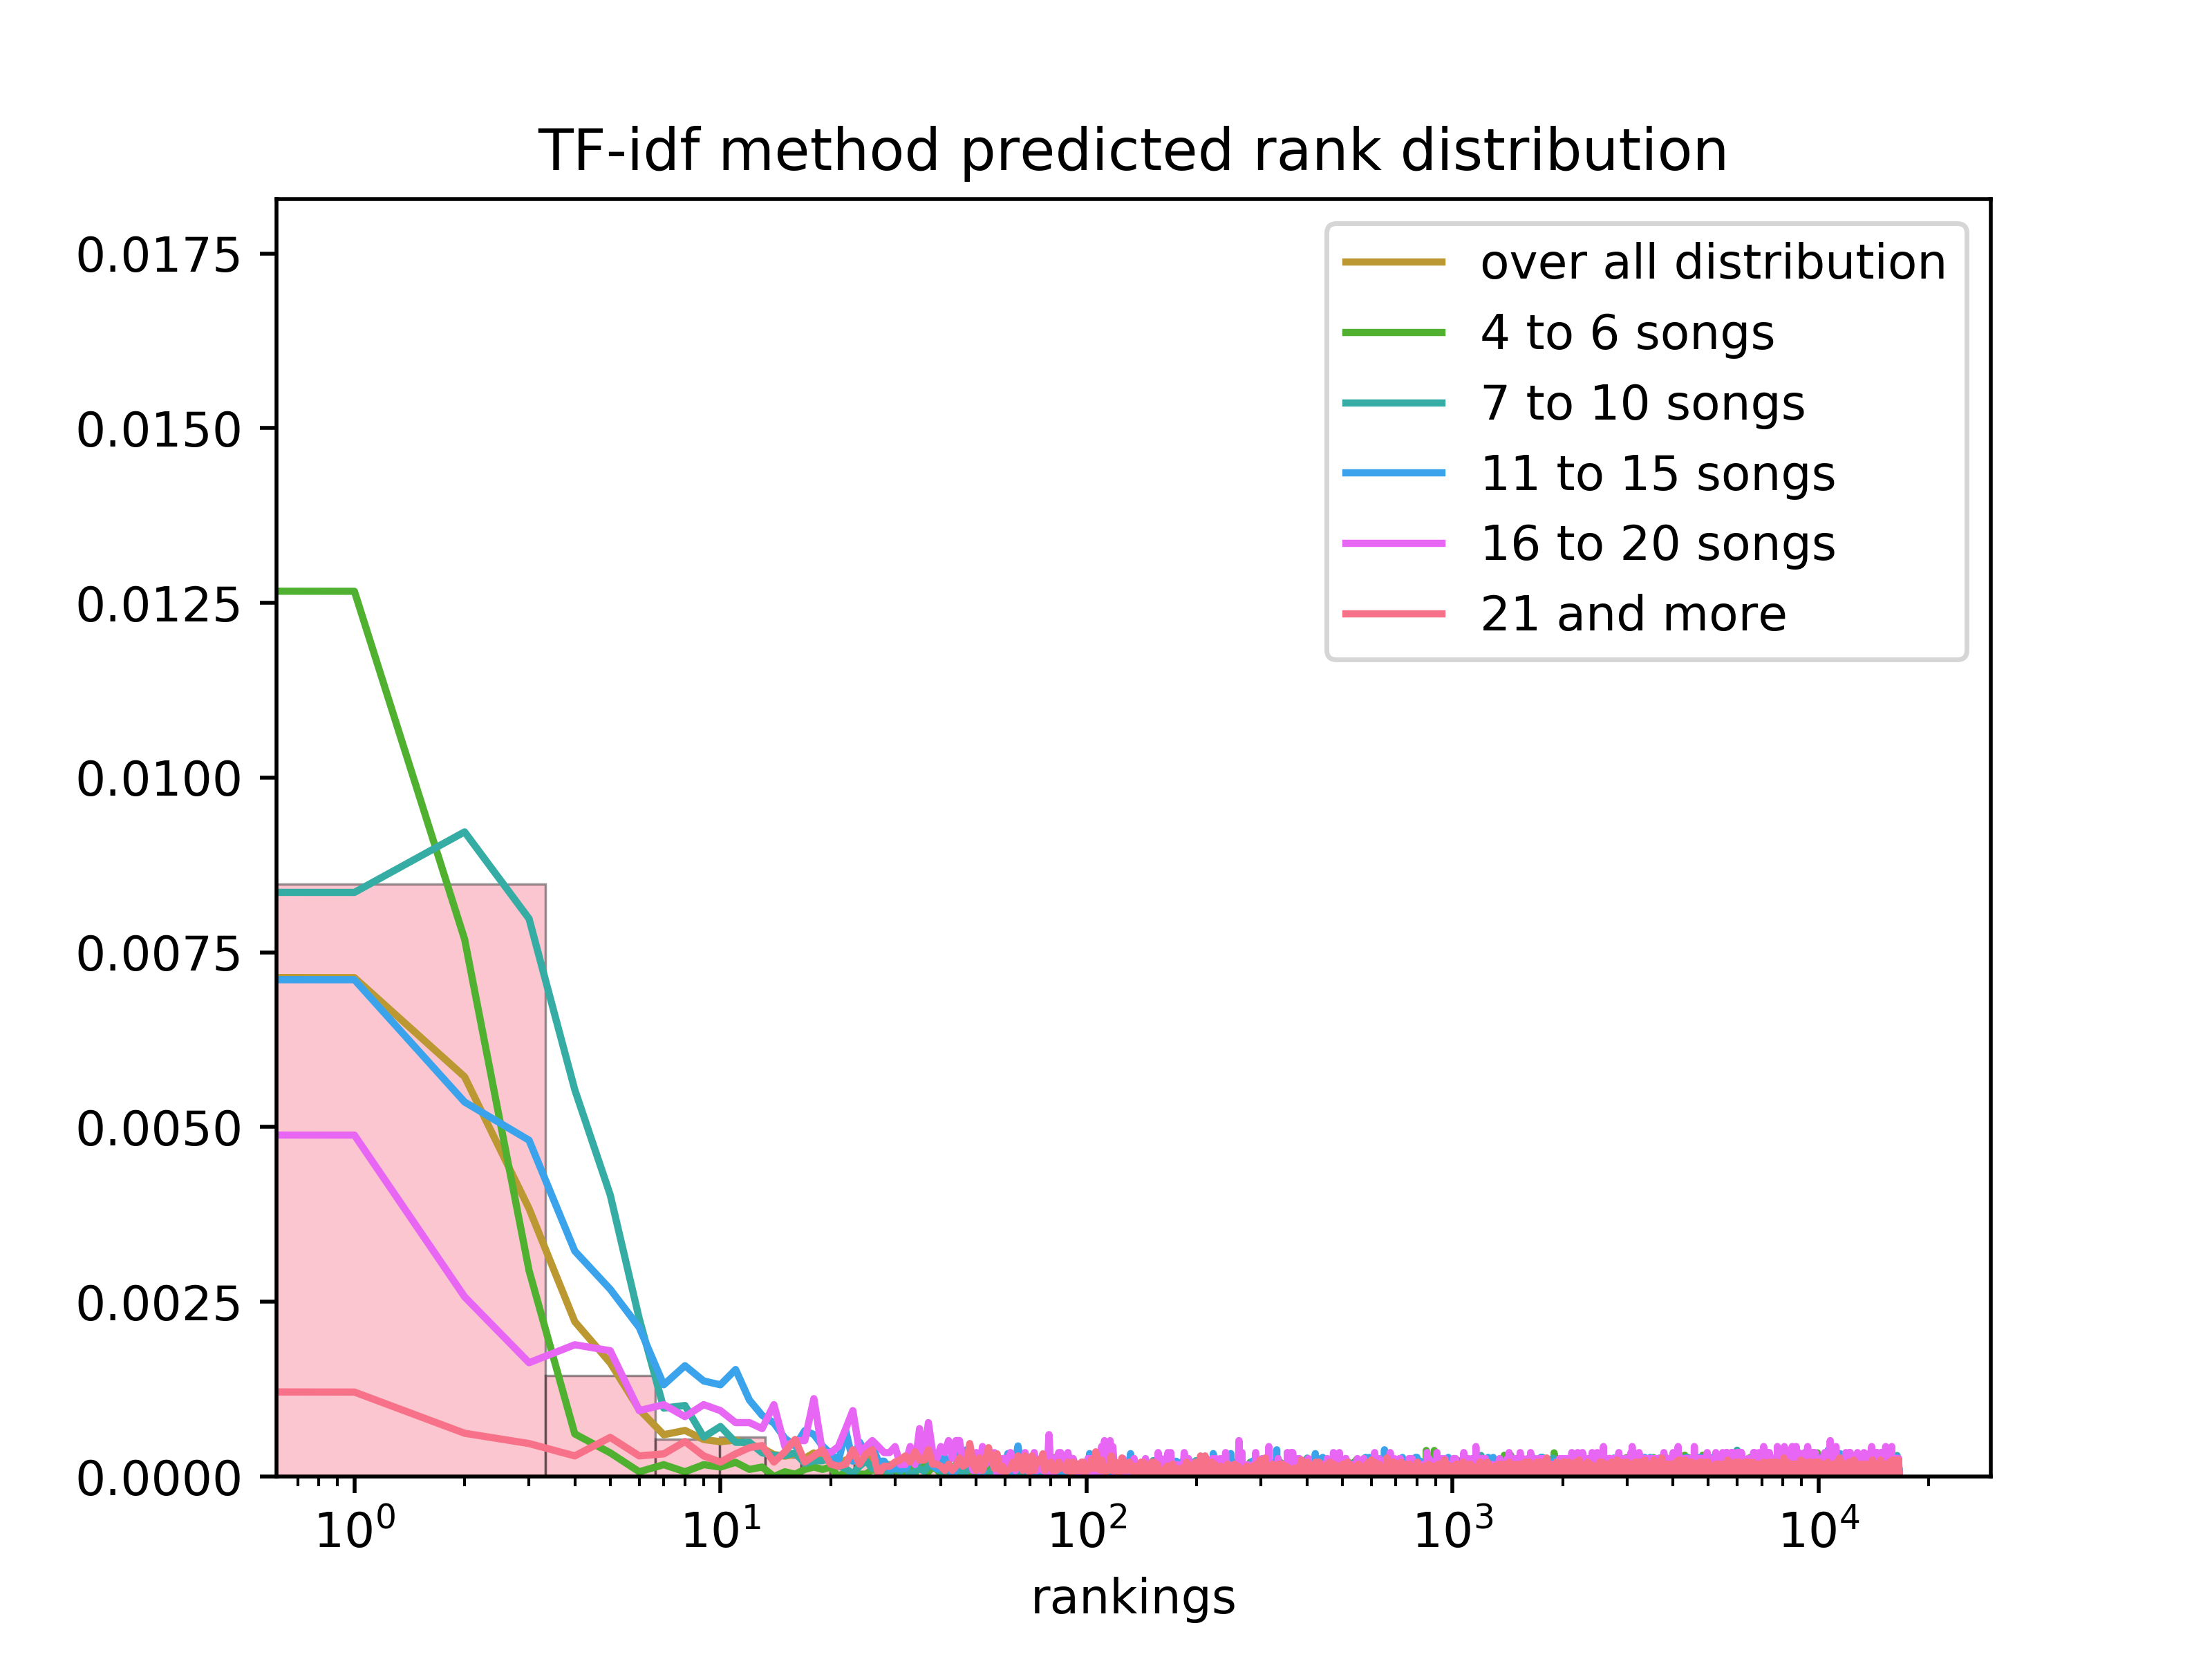
\includegraphics[width=1\linewidth]{./img/tf_idf_graph.png}
  \captionof{Distribution of ranks of songs from the $p_{test}$ set the tf-idf method assigned them.}
  \label{fig:tf_idf_distribution}
\end{minipage}%
\begin{minipage}{.5\textwidth}
  \centering
  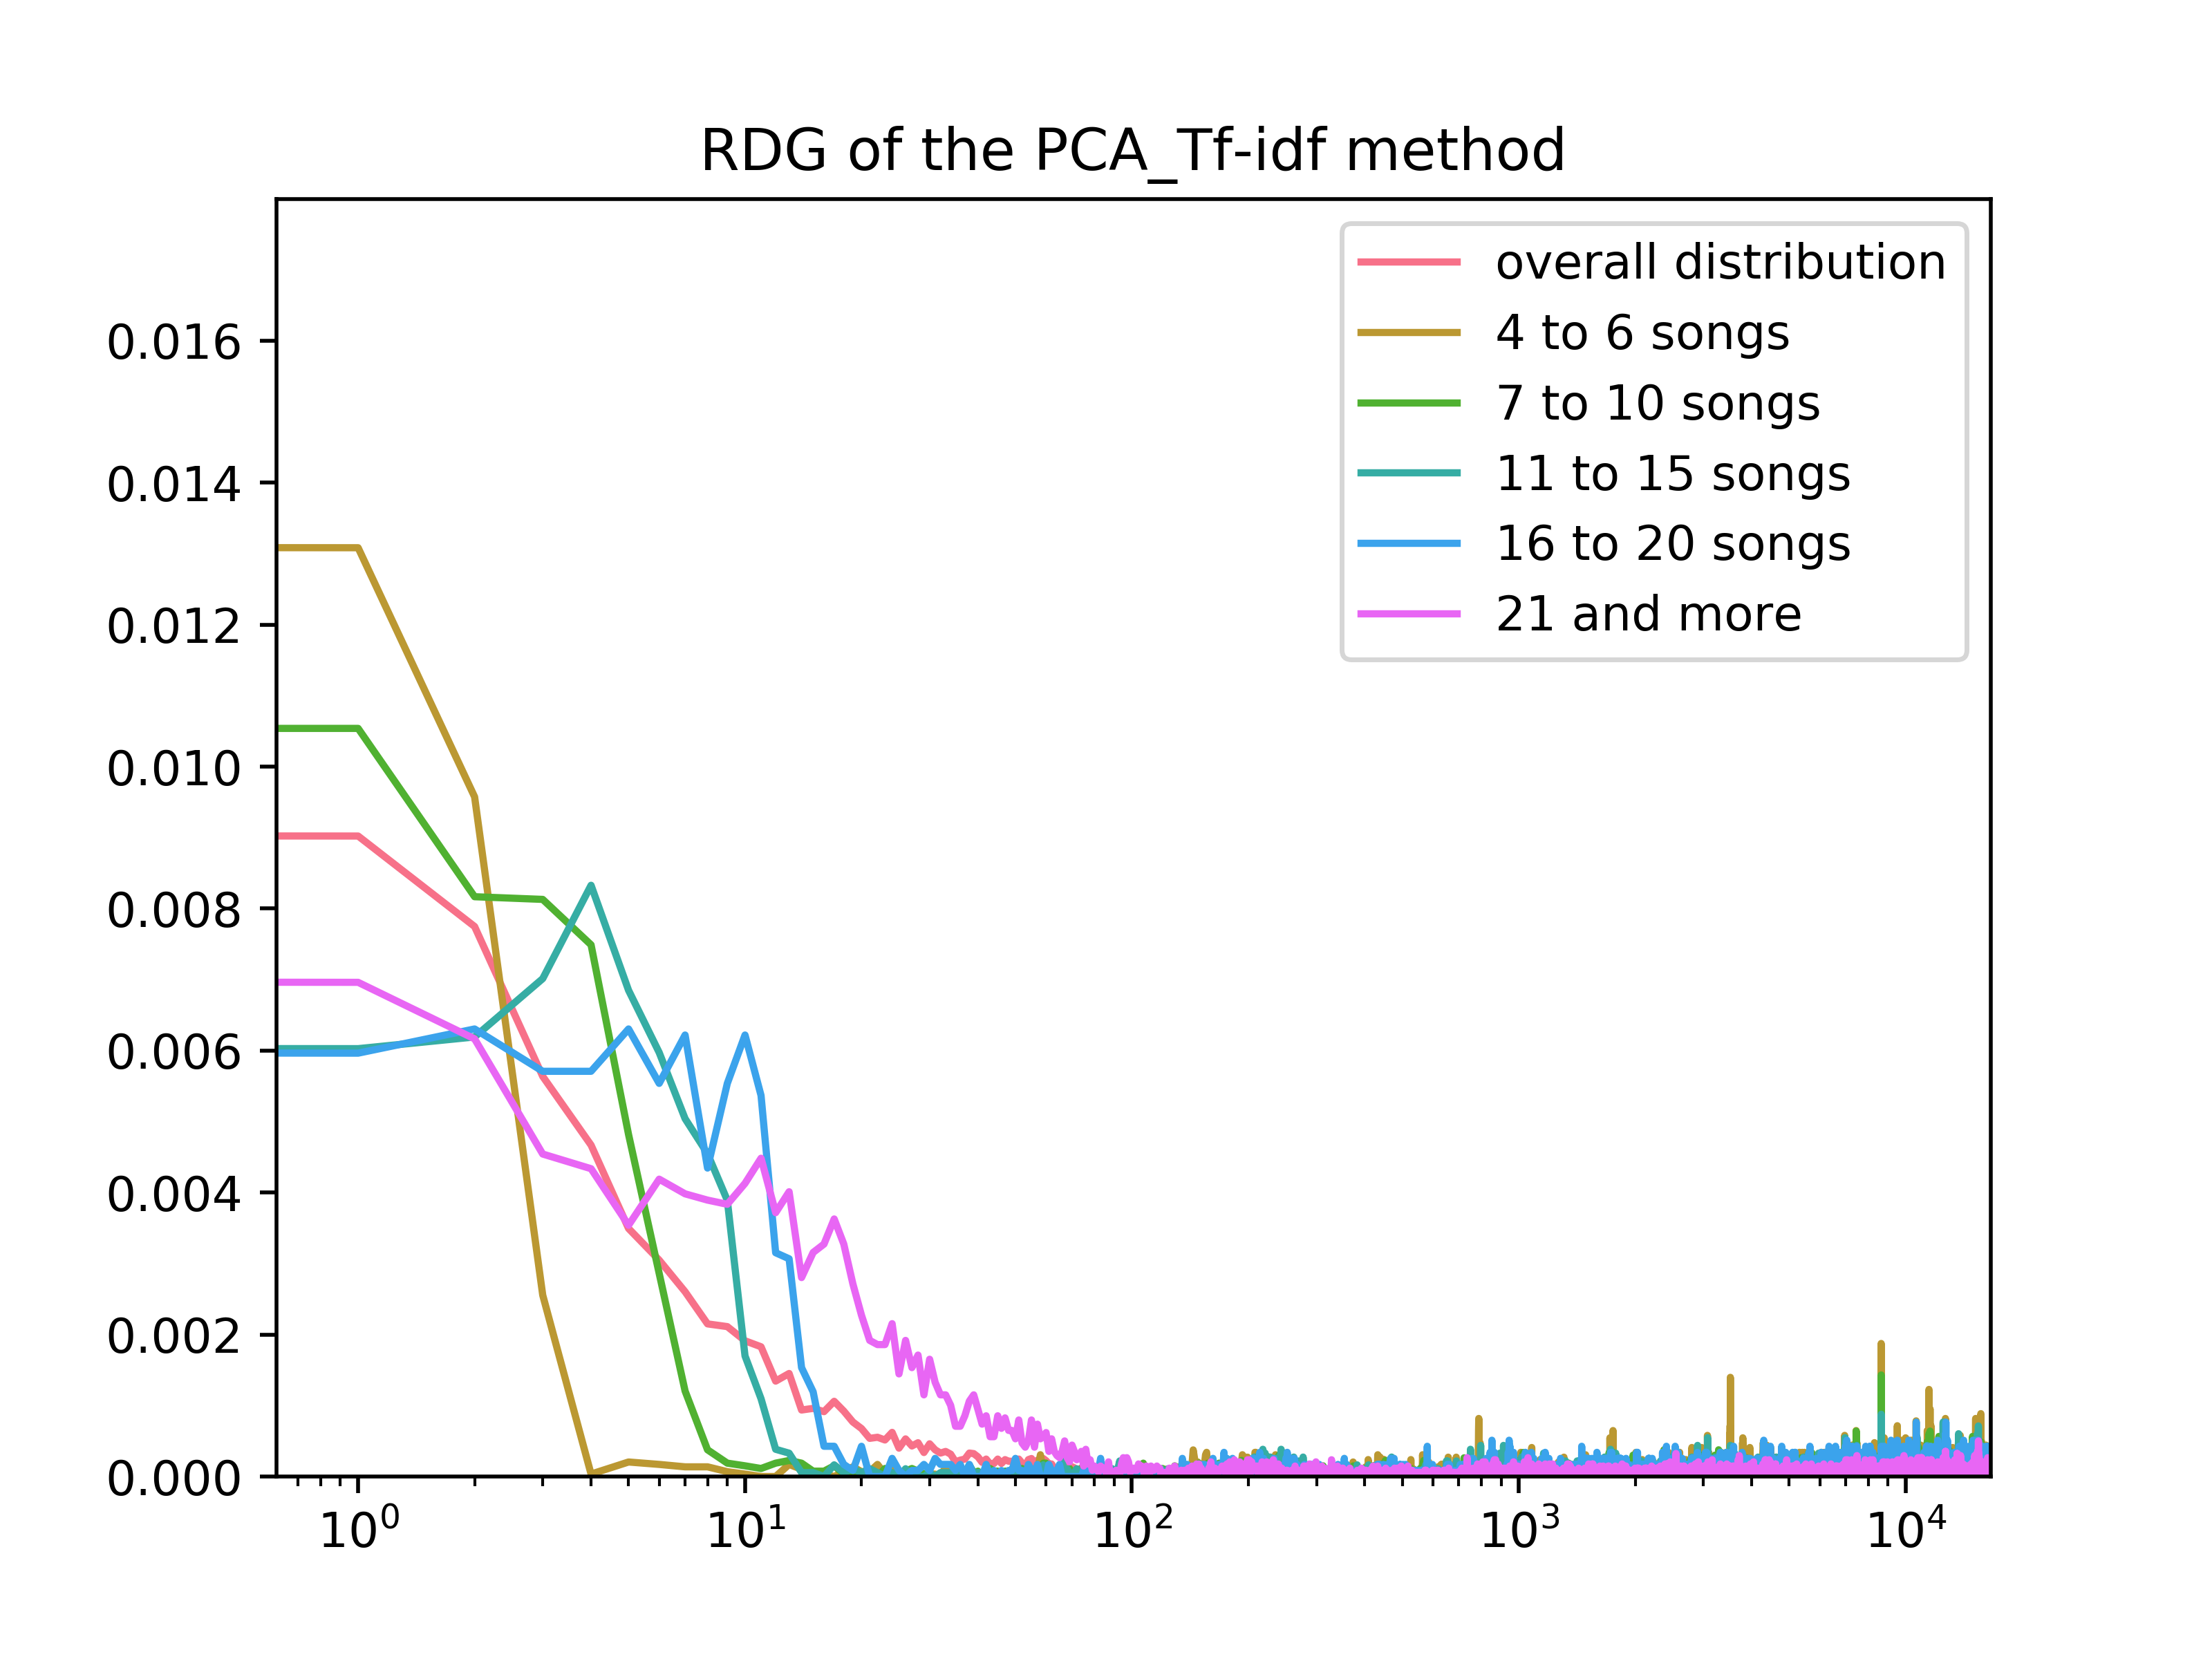
\includegraphics[width=1\linewidth]{./img/pca_tf_idf_graph.png}
  \captionof{Distribution of ranks of songs from the $p_{test}$ for tf-idf vectors as input into PCA}
  \label{fig:pca_tf_idf_distribution}
\end{minipage}
\end{figure}
\subsection{PCA on Tf-idf}\label{ssec:PCA_on_tf_idf}

Because Tf-idf has proven to yield good results we want to implement it. The long vectors pose a problem to our web application though, as it is necessary to calculate the distance between a newly added song and all the songs that are already in the database. Since the machine on which our application is running does not have such computational power as those we run our evaluations on, we decided to try to reduce the dimensions using PCA because has proven quite effective with mel spectrograms.

\subsubsection{Input}
As input, we provided the tf-idf vectors which we acquired as described \ref{ssec:TF_idf}. We did not normalize them.

\subsubsection{Training}
For training we first run a PCA from Python's \texttt{sklearn.decomposition.PCA}. We then chose the space were the explained variance ratio was equal to 90\% which left us with 4457 features. This means, our Tf-idf vector went from 40165 to 4457 dimensions. 

\subsubsection{Output}
The output were vectors of length 4457.

\subsubsection{Results}
The results of the PCA-reduced Tf-idf vector turned out to be better then those of full length. As we can see in \ref{table:1} 

\subsection{Word2Vec experiments}\label{ssec:w2v_experiments}

\subsubsection{Input}
The input for our W2V model was the same as for the Tf-idf method.

\subsubsection{Training}
In the case of Word2Vec, we did not perform any training. Instead, we used a pre-trained W2V model from Google (the first 200000 words which covered all the words in our lyric dataset). If there was a word in a song that is not in our subset added in the web application, would be ignored.

\subsubsectio{Output}
The output for a document of the Google model is a vector of fixed length 300. This is significantly lower than the Tf-idf vector.

\subsubsectio{Results}
The small size of the vectors being produced by the W2V method are a significant advantage of this method. However the results it yielded make it below average even compared to our other methods.

\begin{table}[h!]
\centering
\renewcommand{\arraystretch}{1.5}
\begin{tabu} to 1\textwidth { | c || X[c] | X[c] | X[c] | X[c] | X[c] |}
 \hline
 \textbf{method} & \textbf{R@10} & \textbf{R@50} & \textbf{R@100} & \textbf{nGDC} & $ \boldsymbol{\overline{rank}} $ \\
 \hline
 \hline
 W2V & 0.00768 & 0.01354 & 0.01983 & 0.00909 & 7682 \\
 \hline
\end{tabu} \\
\caption{Table summarizing average W2V values averaged over the 5 cross validation that were performed}
\label{table:2}
\end{table}

The table shows much lower numbers than for the Tf-idf method. Only 0.7\% of songs from the $ p_{test} $ set ranked in the top 10, 1.3\% in top 50 and 2.0\% in top 100. The average rank was 7682. That does not seem to be as bad compared to Tf-idf so it suggests that the songs did not place at the last ranks, but also not at the first ranks. \\
When looking at the distribution graph, it is very clear that the gap here between the accuracy of predicted ranks for short and longer playlists is huge. Although not great, it performs much better for short playlists. For playlists as short as 7, the performance drops significantly and it appears that for playlists with length 11 and more, the trend is opposite than what we would want, meaning, that it is more likely that a song from the $p_{test}$ set does ranks between the last 1000 than between the first 1000 if the rank is predicted based on a playlists of length at least 11.

\begin{figure}[h]
    \centering
	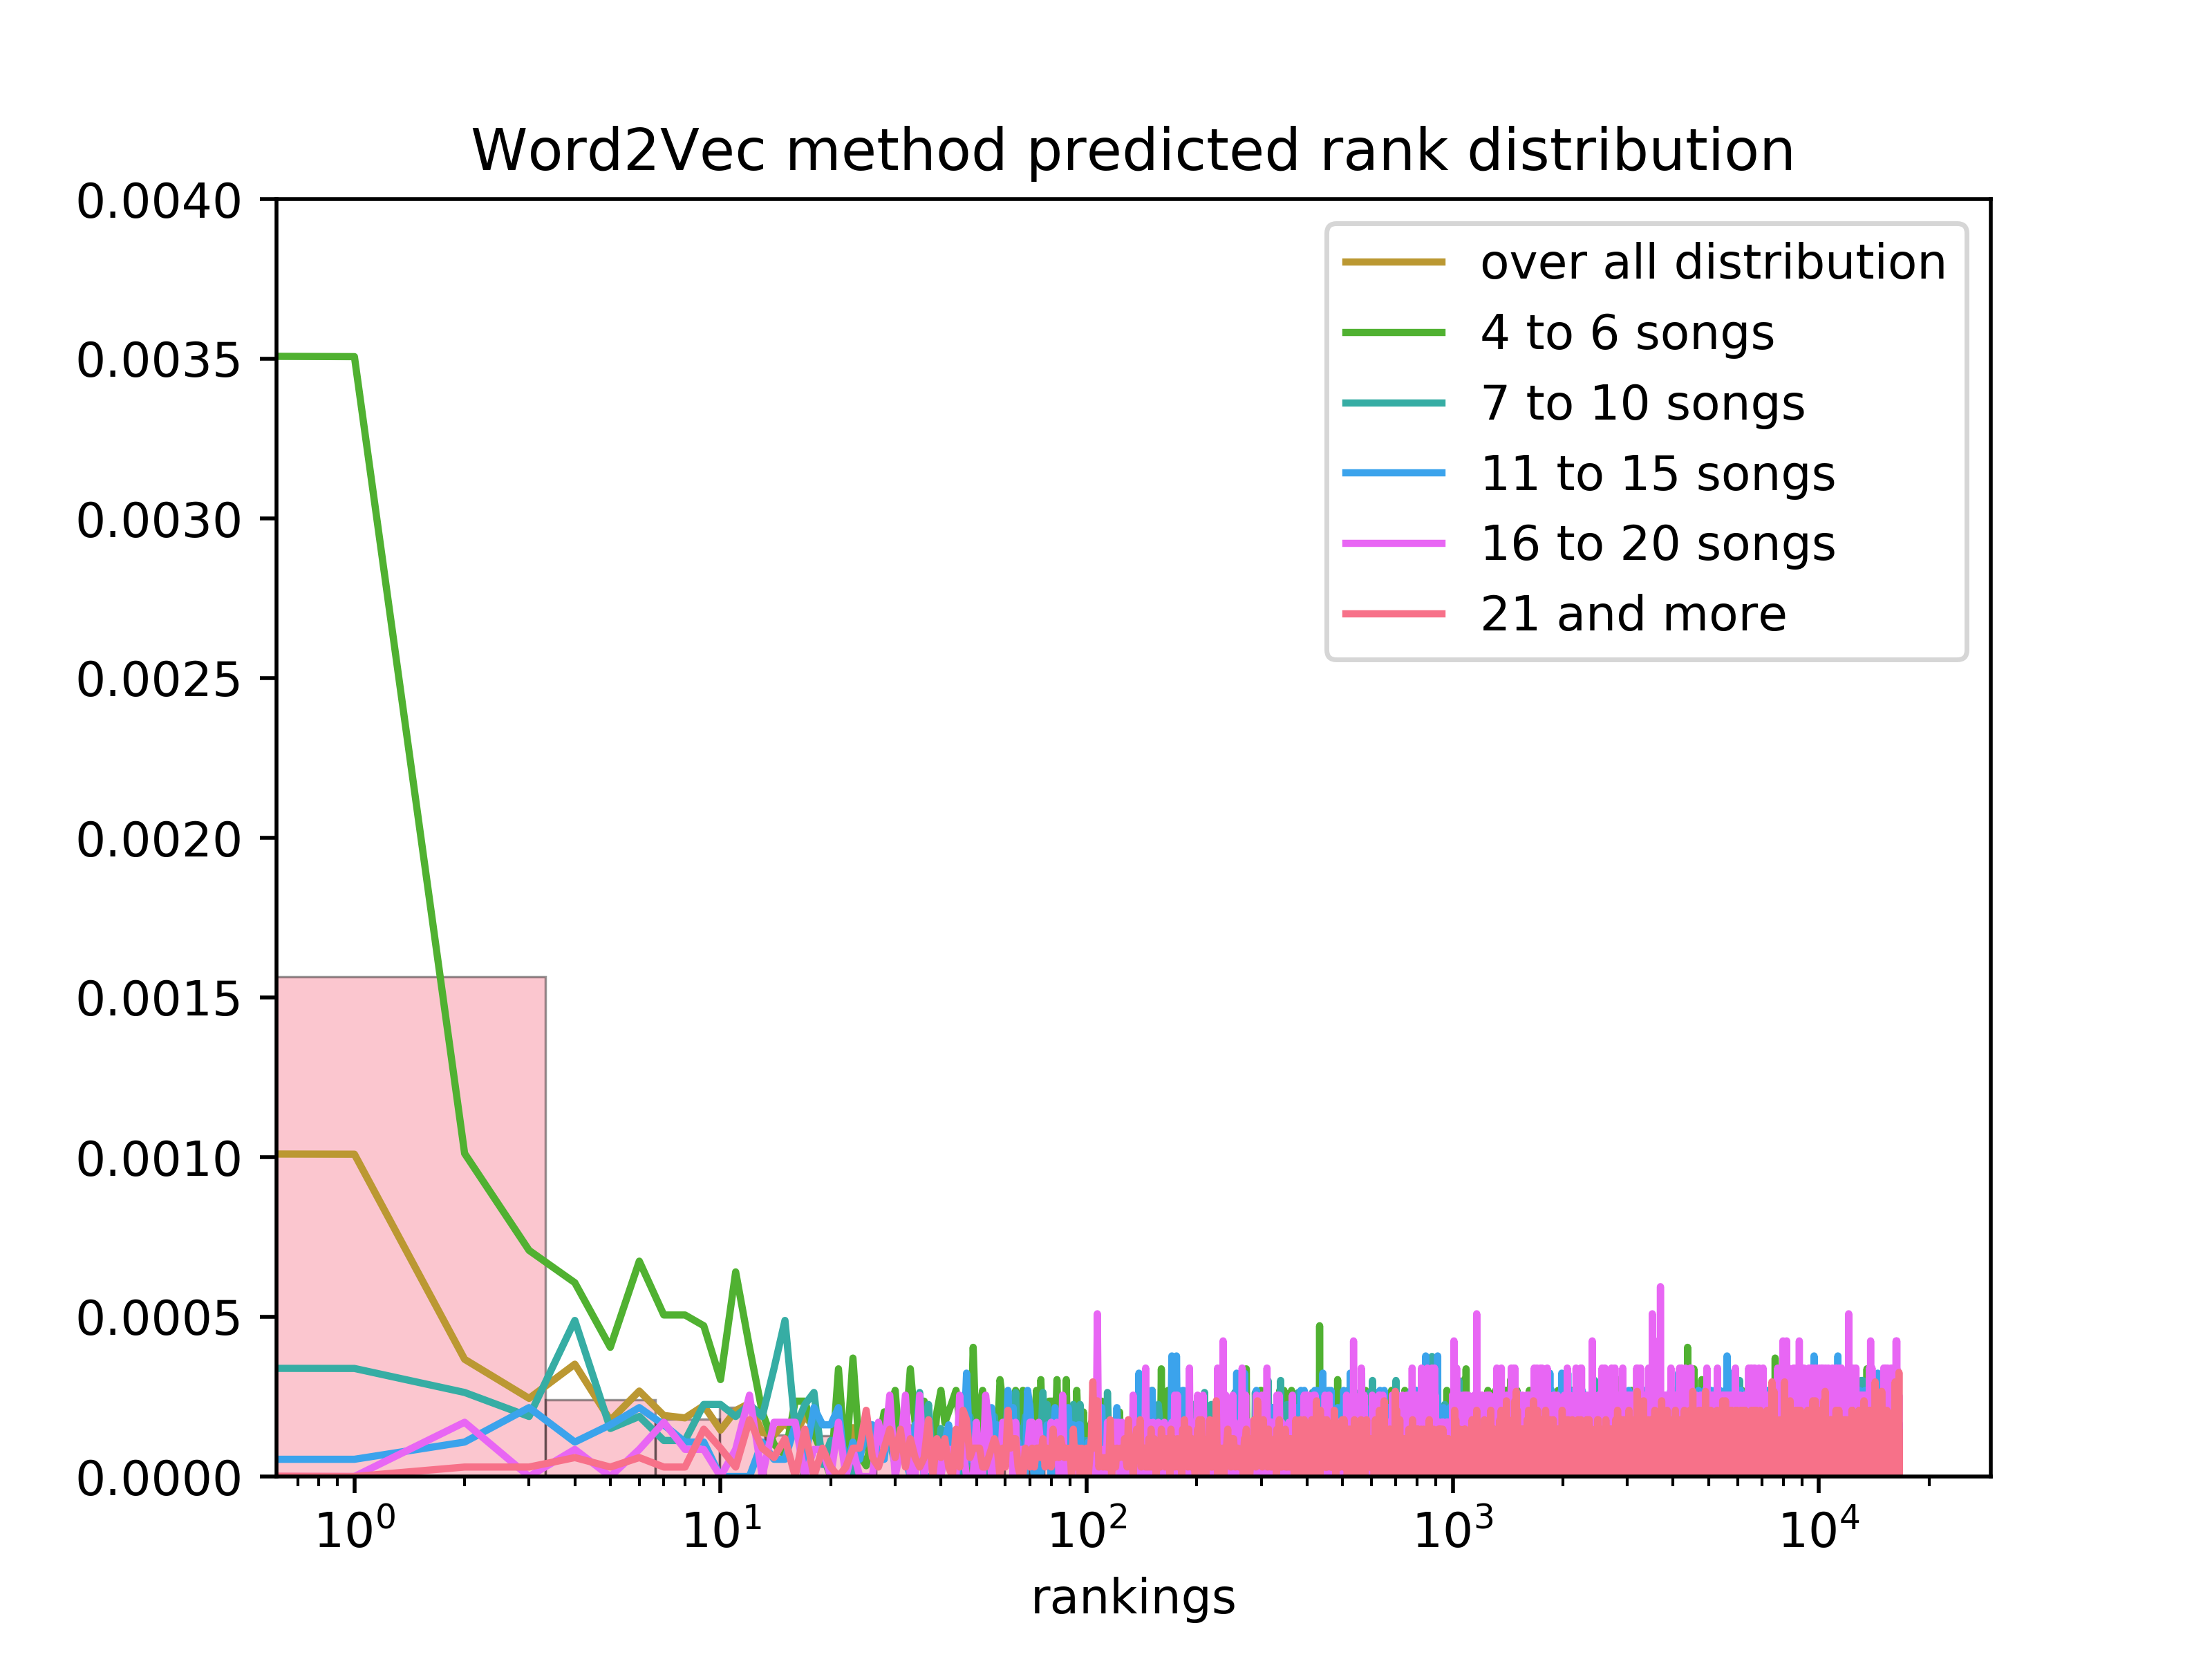
\includegraphics[width=120mm]{./img/w2v_graph.png}
	\caption{Distribution of ranks of songs from the test set the w2v method assigned them.}
	\label{fig:w2v_distribution}
\end{figure}

\subsection{SOM experiments}
We used a python library called \texttt{minisom} \cite{Vettigli2019}
\subsubsection{Input}
We tried the W2V vectors from \ref{ssec:w2v_experiments} as input for our self organizing map, mainly because of their length and also because we were hoping, that the SOM could improve the results of the W2V method. We also tried to train the SOM on the output vectors of our PCA\_Tf-idf method. We did not try the raw Tf-idf vectors as they are long and it would prolong training significantly and also, because the PCA\_Tf-idf yielded better results than raw Tf-idf.

\subsubsection{Training}
We build a self organizing map with a grid size 5 times our dataset size (16594) and the number of iterations was also 5 times our dataset size. We saved a model after each multiple of 16594 iterations and interestingly, the representations did not change after 33 187 iterations (meaning 2*16594). It was also necessary to normalize our input vectors and set learning rate to 0.2. Otherwise the songs formed 3 to 5 large clusters on the grid placing thousands of songs on the same coordinate. 
\subsubsection{Output}
The output representation for each song was a vector of length two. The whole dataset then could be displayed on a 2D map. 
When we then tried to display the map with all the songs, the size of the image would have to be immense so that all 16594 songs would be recognizable. The problem was that there were many songs to display on the map and the titles overlapped. Because of that, we decided to randomly select 20 playlists and show where the different songs that belong to each playlist placed on the map. Each playlist has its own color. This map for the W2V input is depicted in \ref{fig:som_map}. Obviously, the playlists do not really form any visible clusters.
\begin{figure}[h]
    \centering
	\includegraphics[width=140mm]{./img/som_map.png}
	\caption{The location of different songs from 20 randomly selected playlists on the map created by SOM. Each playlist has its own colour.}
	\label{fig:som_map}
\end{figure}
\subsubsection{Results}
The fact that the playlists do not form clusters is also supported by the fact that the overall results for the self organizing map algorithm are quite poor. Actually it is the worse method that we implemented and our hope to improve the results of W2V were not fulfilled.

\begin{table}[h!]
\centering
\renewcommand{\arraystretch}{1.5}
\begin{tabu} to 1\textwidth { | c || X[c] | X[c] | X[c] | X[c] | X[c] |}
 \hline
 \textbf{method} & \textbf{R@10} & \textbf{R@50} & \textbf{R@100} & \textbf{nGDC} & $ \boldsymbol{\overline{rank}} $ \\
 \hline
 \hline
 SOM with W2V & 0.00084 & 0.0038 & 0.00664 & 0.00192 & 8152 \\
 \hline
 SOM wiht PCA_Tf-idf & 0.000435 & 0.002084 & 0.004621 & 0.001254 & 8243 \\
 \hline
\end{tabu} \\
\caption{Table summarizing average SOM values averaged over the 5 cross validations}
\label{table:som}
\end{table}
The distribution graph of the SOM\_W2V method clearly shows, that the distribution of ranks is random or worse which is also suggested by the fact that the average rank is 8152 which almost in the middle of 16594. The main reason for the failure of this method is unclear but it is possible that the data from the W2V vectors that already contain too little information for the SOM network to be able to cluster data based on it.  But since we recieved even worse results for the SOM\_Tf-id we are more inclined to another possibility which is, that the SOM network is not be able to provide satisfying results because two dimensions are simply too little to represent the whole complexity of the input data.
\begin{figure}[h]
    \centering
	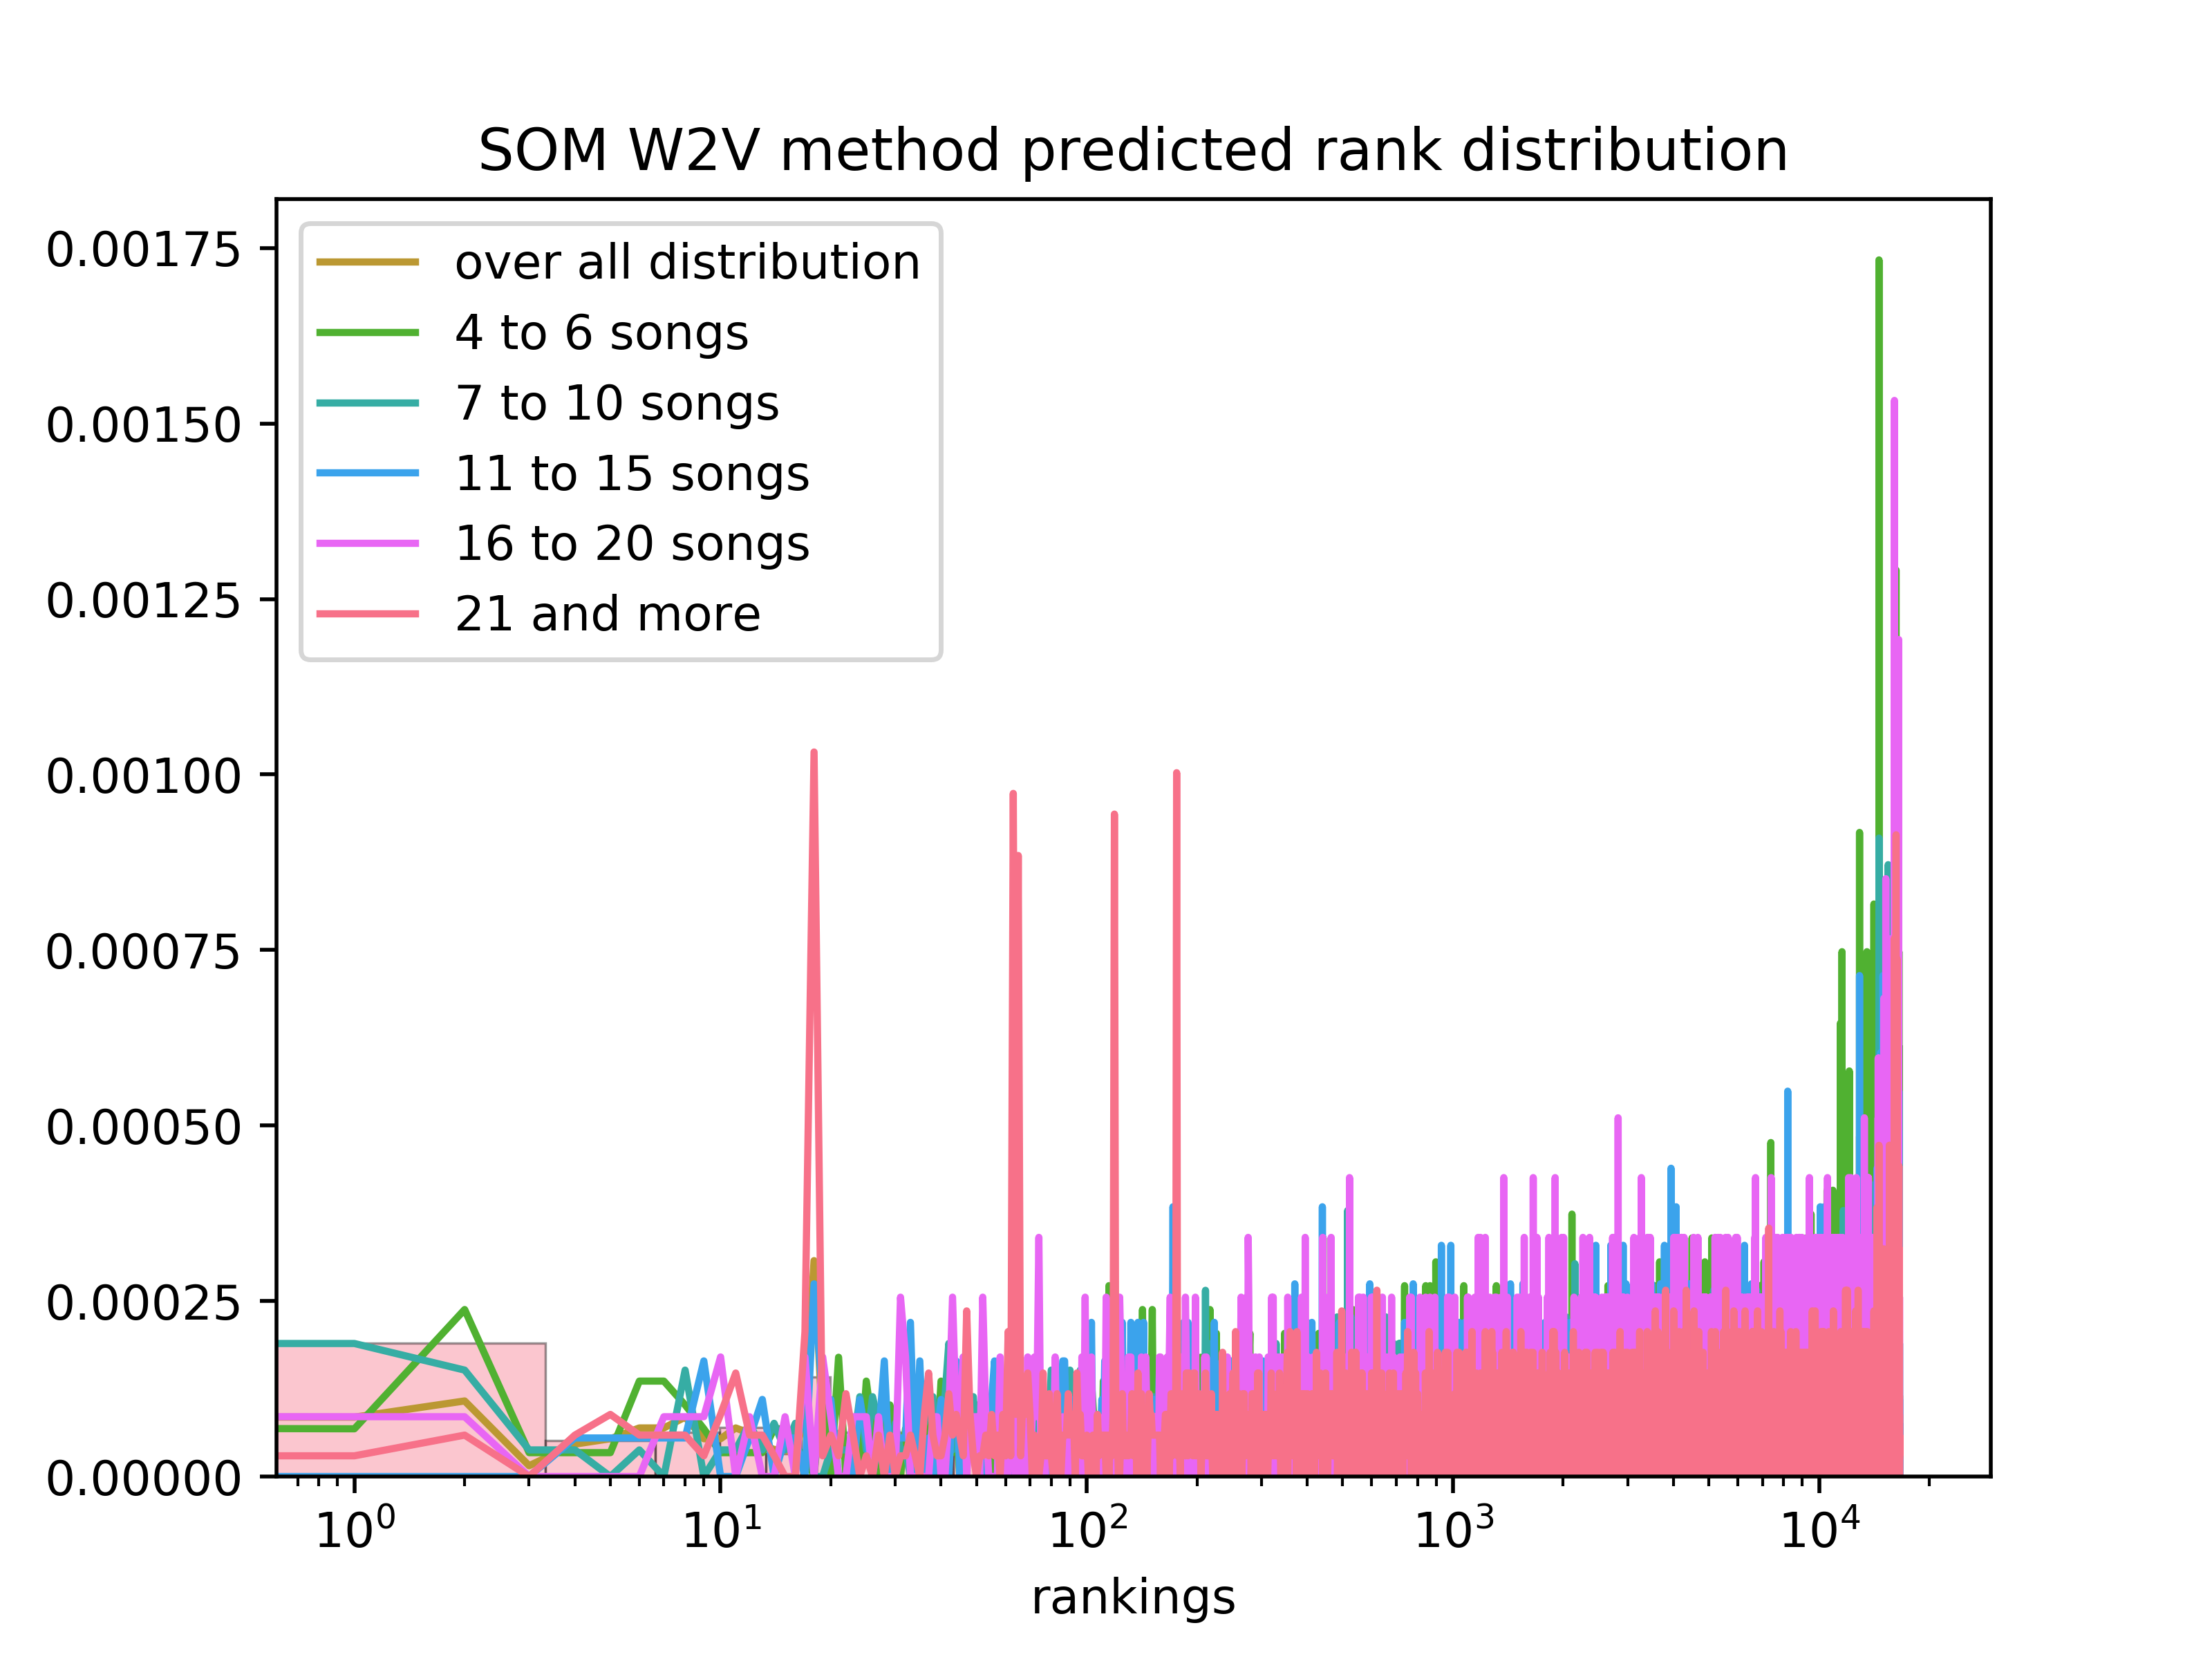
\includegraphics[width=120mm]{./img/som_w2v_graph.png}
	\caption{Distribution of ranks of songs from the test set the SOM method assigned them.}
	\label{fig:som_distribution}
\end{figure}
\section{Simple audio method experiments}
\subsection{Audio preparation}\label{ssec:audio_prep}

In order to encode audios of songs, we first needed to acquire some form of the music to become our standard. To make our audio information suitable for machine learning, we decided to extract audios of the same length so our vectors (spectrograms, mel-spectrograms and mfccs are also of the same length). Since all songs have different lengths and also, one complete 3.5 minute long song results in a spectrogram of size 5214x2206 which when flattened is a vector of length 11 502 084. Therefore we decided to extract 15 second excerpts from each song to create spectrograms, mel-spectrograms and MFCCs from those. We took 5 seconds between the 15th and 20th second, 5 seconds starting in the middle of the song and 5 second starting 15 seconds before the end. We did not start at the beginning and the end because in some songs, there is silence or applause or some talking before the actual song starts. \\

It was also necessary to decide on some parameters for spectrograms, mel-spectrograms and MFCCs. As stated previously, our neural networks were inspired by \cite{inproceedings_RNNs} where they also performed parameter optimisation. We decided to use their parameters as input for all our methods. It is possible that some parameters values suite some methods better than others but because of the amount of methods we tested we decided it would too difficult to optimise them for each method. We also think, that it a good idea to have all methods work with more or less the same input as their comparison is less ambiguous. \\
The resulting choices were following. We set window width $w$ to 0.2 and window overlap $w_o$ to 0.5$w$ = 0.1. For mel-spectrograms it is also necessary to choose Mel frequency bands which was set to 320 as for values above 320, the performance of neural networks did not increase. For MFCC coefficients we decided to set the number of MFCC coefficients to 320 which is the same as the number of Mel frequency bands.

We used Python's \texttt{librosa} library \cite{brian_mcfee_2019_2564164} to cut our songs and to generate our spectrograms, mel spectrograms and MFCCS using functions \texttt{librosa.core.stft} for spectrograms \texttt{librosa.feature.mel\_spectrogram} for mel-spectrograms and \texttt{librosa.feature.mfcc} for MFC coeficients. The audio data for training was stored in .wav files.

\subsection{Raw Mel spectrograms}\label{ssec:raw_mels}
The input for mel spectrograms was the 15 second long audio described in \ref{ssec:audio_prep}. Extracting spectrograms does not require any training. It a is mathematical procedure explained in \ref{ssec:mel_spectrograms_intro}.

The mel-spectrograms we got after transforming a 15 second long audio with 320 Mel frequencies bands was a matrix of size 408x320 which when flattened is a vector of size 130560. This turned out to be too long to implement in our application, however because we did not realize that at first, we tested this method and got the following results. \\
As can be seen in \ref{table:mel_spec_methods} 3.7\% of songs ended up between top ten predictions, 4.3\% in top 50 and 4.7\% in the top 100. These results are actually better than any other method using mel-spectrograms as input except of PCA. It beats both neural network architectures with mel-spectrogram input. 

\subsubsectio{Results}
\begin{table}[h!]
\centering
\renewcommand{\arraystretch}{1.5}
\begin{tabu} to 1\textwidth { | c || c | c | c | c | c |}
 \hline
 \textbf{method} & \textbf{R@10} & \textbf{R@50} & \textbf{R@100} & \textbf{nGDC} & $ \boldsymbol{\overline{rank}} $ \\
 \hline
 \hline
 Raw mel spectrograms & 0.03696 & 0.04275 & 0.0473 & 0.03063 & 7604 \\
 \hline
 PCA_mel_5715 & 0.05243 & 0.06153 & 0.06737 & 0.04300 & 6851 \\
 \hline
 PCA_mel_320 & 0.00053 & 0.00196 & 0.00633 & 0.00155 & 8357 \\
 \hline
 GRU_mel  & 0.03623 & 0.04336 & 0.04870 & 0.03119 & 7601 \\
 \hline
 LSTM_mel & 0.01368 & 0.02028 & 0.02579 & 0.01423 & 7861\\
 \hline
\end{tabu} \\
\caption{Table summarizing average rank values for all methods with mel-spectrogram input averaged over the 5 cross validations}
\label{table:mel_spec_methods}
\end{table}
  
The patterns observed in \ref{fig:mel_graph} which shows the distribution of ranks for raw mel-spectrograms is similar to all other methods we are studying (except of those that appear to be random such as SOM). The ranking is better when predicting ranks of songs from shorter playlists. 

\begin{figure}[h]
    \centering
	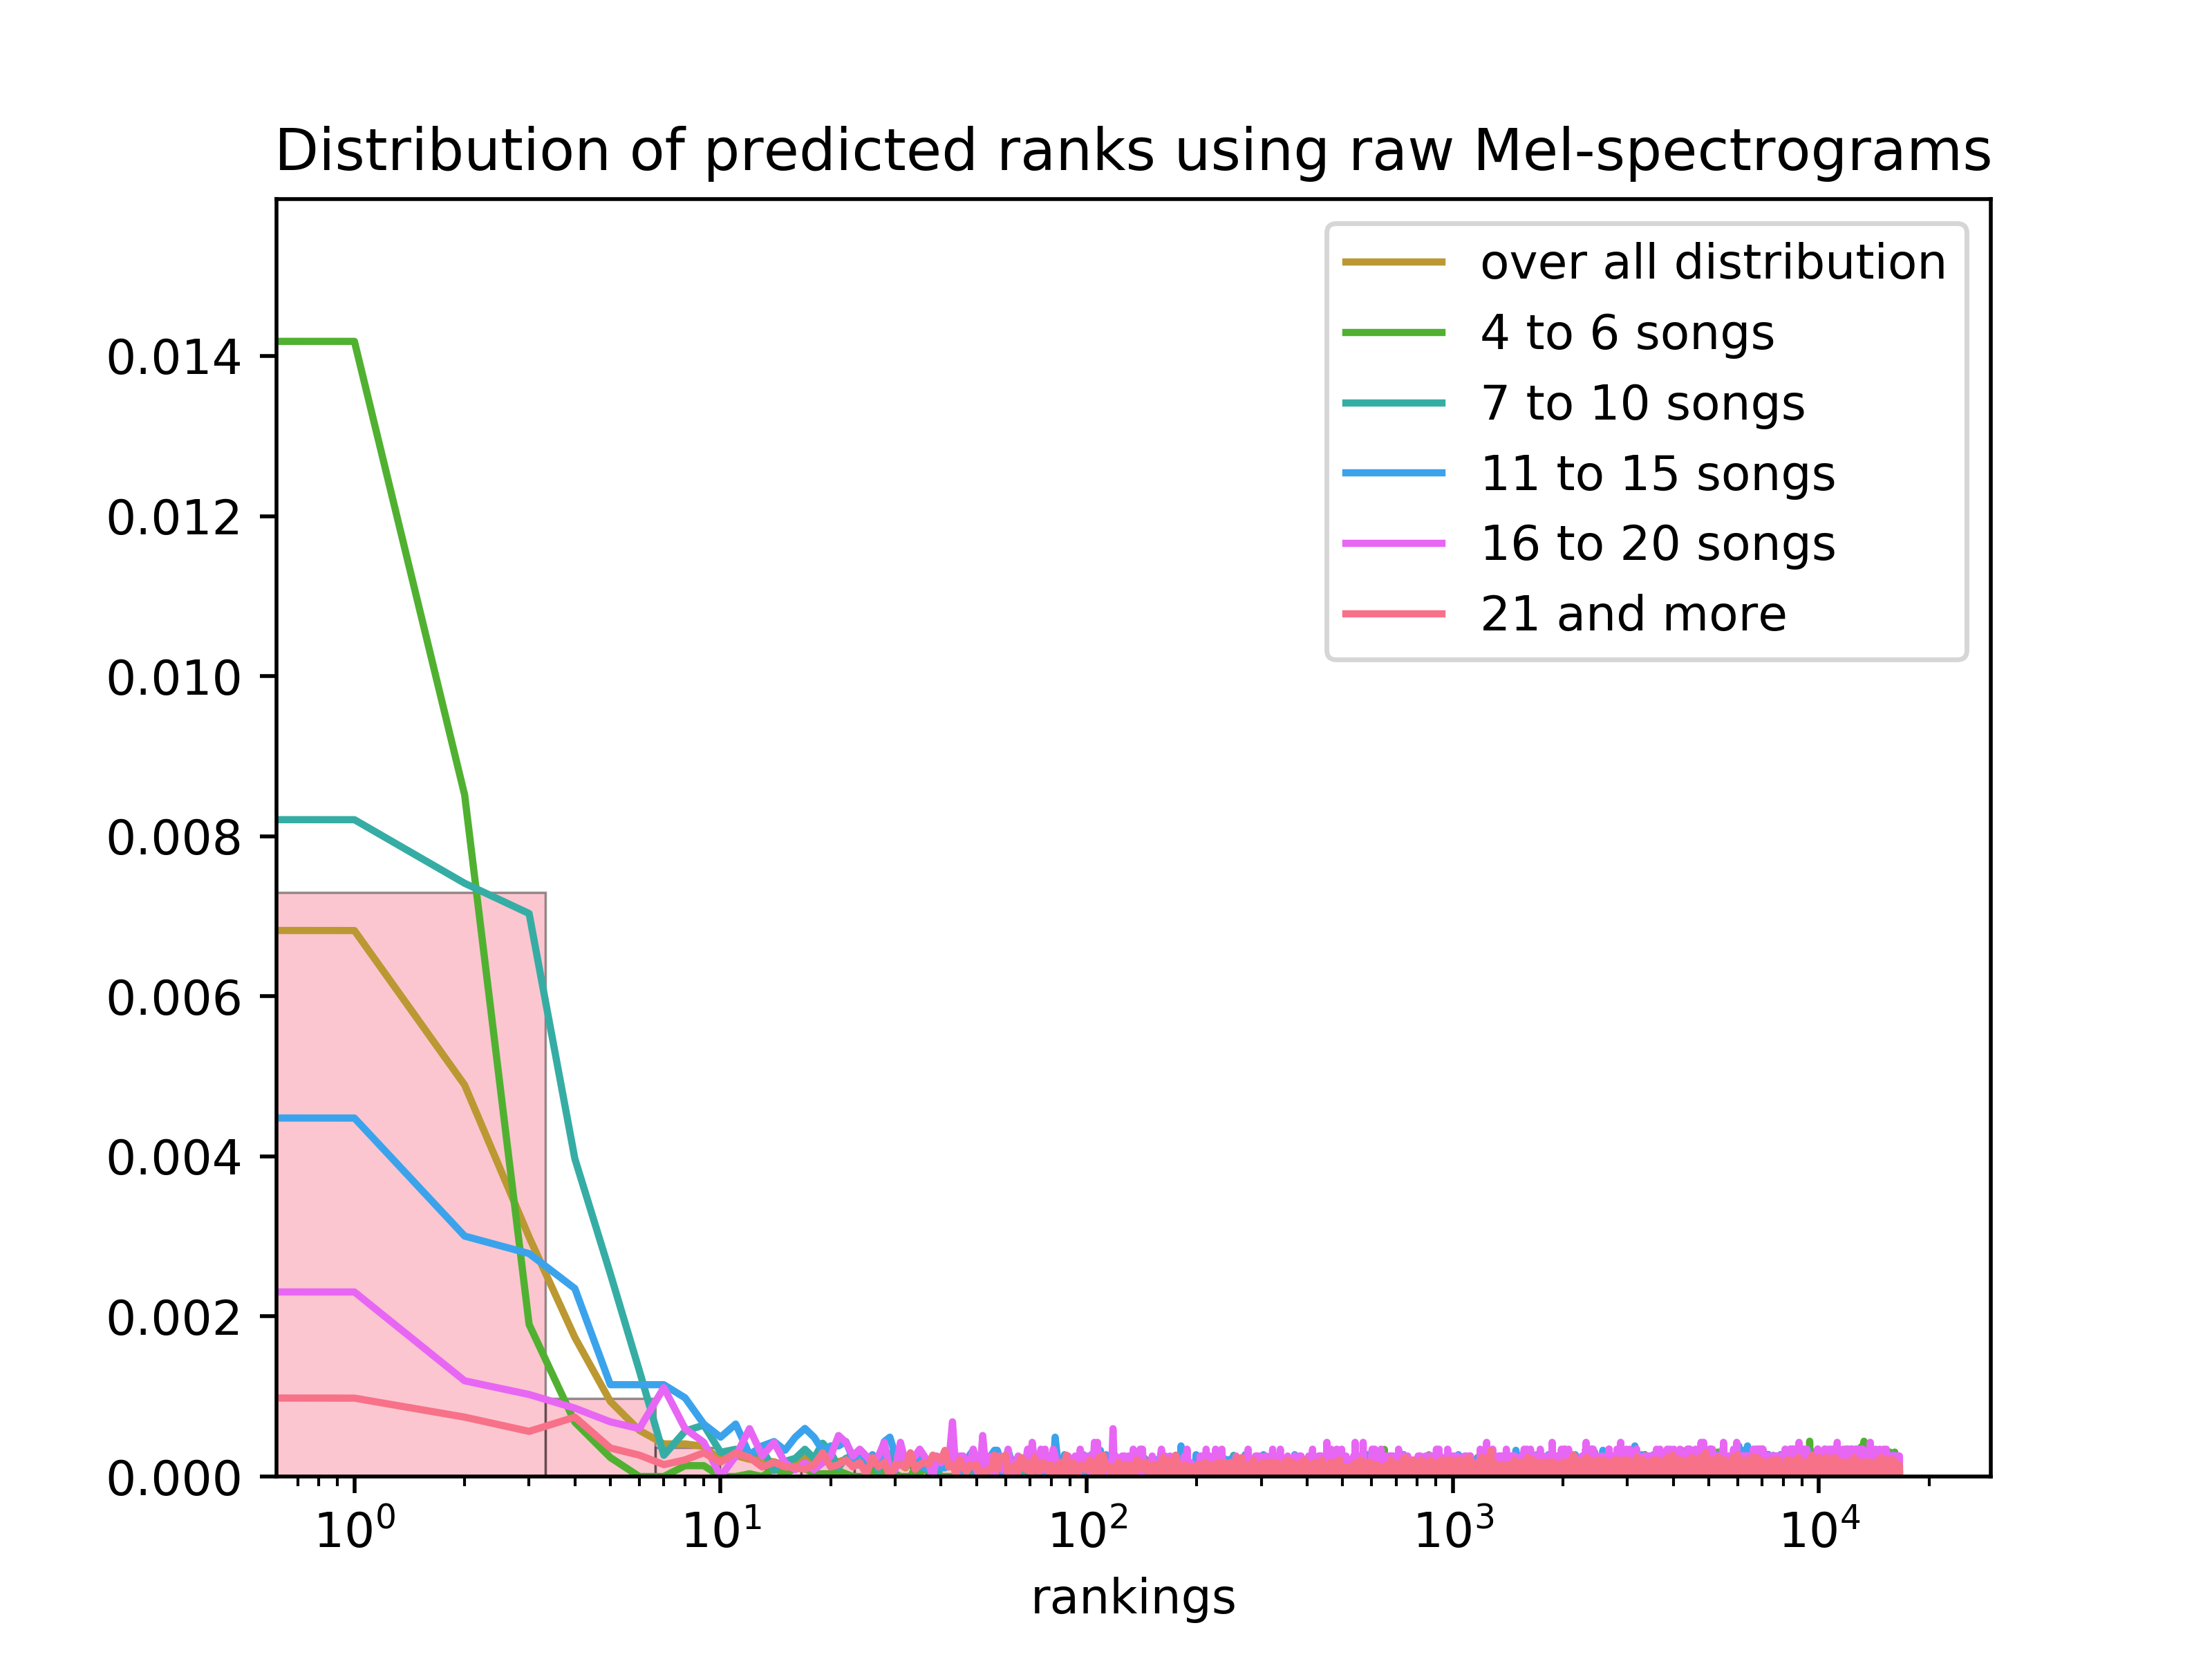
\includegraphics[width=120mm]{./img/mel_graph.png}
	\caption{Distribution of ranks of songs from the test with their similairity defined as cosine distance between mel-spectrograms.}
	\label{fig:mel_graph}
\end{figure}

\subsection{Raw MFCCs}
Our 15 second audios were fed as input into the texttt{librosa.feature.mfcc()} function with parameters mentioned in \ref{ssec:audio_prep}. Training was not necessary since acquiring mel-frequency cepstral coefficient is a matter of Fourier Transformations and the resulting matrix had the shape of 646x128. When flattened we get a vector of length 82866. This has proven to be too long for practical use in our application, however we still have the evaluation results when defining song similarity as the cosine distance between flattened MFCC matrices.

\subsubsection{Results}

The results of MFCCs are quite poor even compared to our other methods. Only 0.4\% of songs missing in our playlists rank betwen the top 10, 0.9\% in the top 50 and 1.4\% in the top 100. However as can be seen in table \ref{table:mfcc_methods} it is better than when using mfc coefficients with our LSTM network.
\begin{table}[h!]
\centering
\renewcommand{\arraystretch}{1.5}
\begin{tabu} to 1\textwidth { | c || X[c] | X[c] | c | X[c] | X[c] |}
 \hline
 \textbf{method} & \textbf{R@10} & \textbf{R@50} & \textbf{R@100} & \textbf{nGDC} & $ \boldsymbol{\overline{rank}} $ \\
 \hline
 \hline
 Raw MFCC & 0.00415 & 0.00919 & 0.01423 & 0.00607 &  7552 \\
 \hline
 LSTM\_MFCC & 0.00246 & 0.00674 & 0.0116 & 0.00436 & 7665 \\
 \hline
 GRU\_MFCC & 0.00510 & 0.01148 & 0.01755 & 0.00721 & 7391 \\
 \hline
\end{tabu} \\

\caption{Table summarizing average rank values for all methods with MFCC input averaged over the 5 cross validations}
\label{table:mfcc_methods}
\end{table}

 When looking at our traditional distribution graph, we again observe the a lower probability of good song rankings as the length of playlists increases. Again completely against what we hope for. 
\begin{figure}[h]
    \centering
	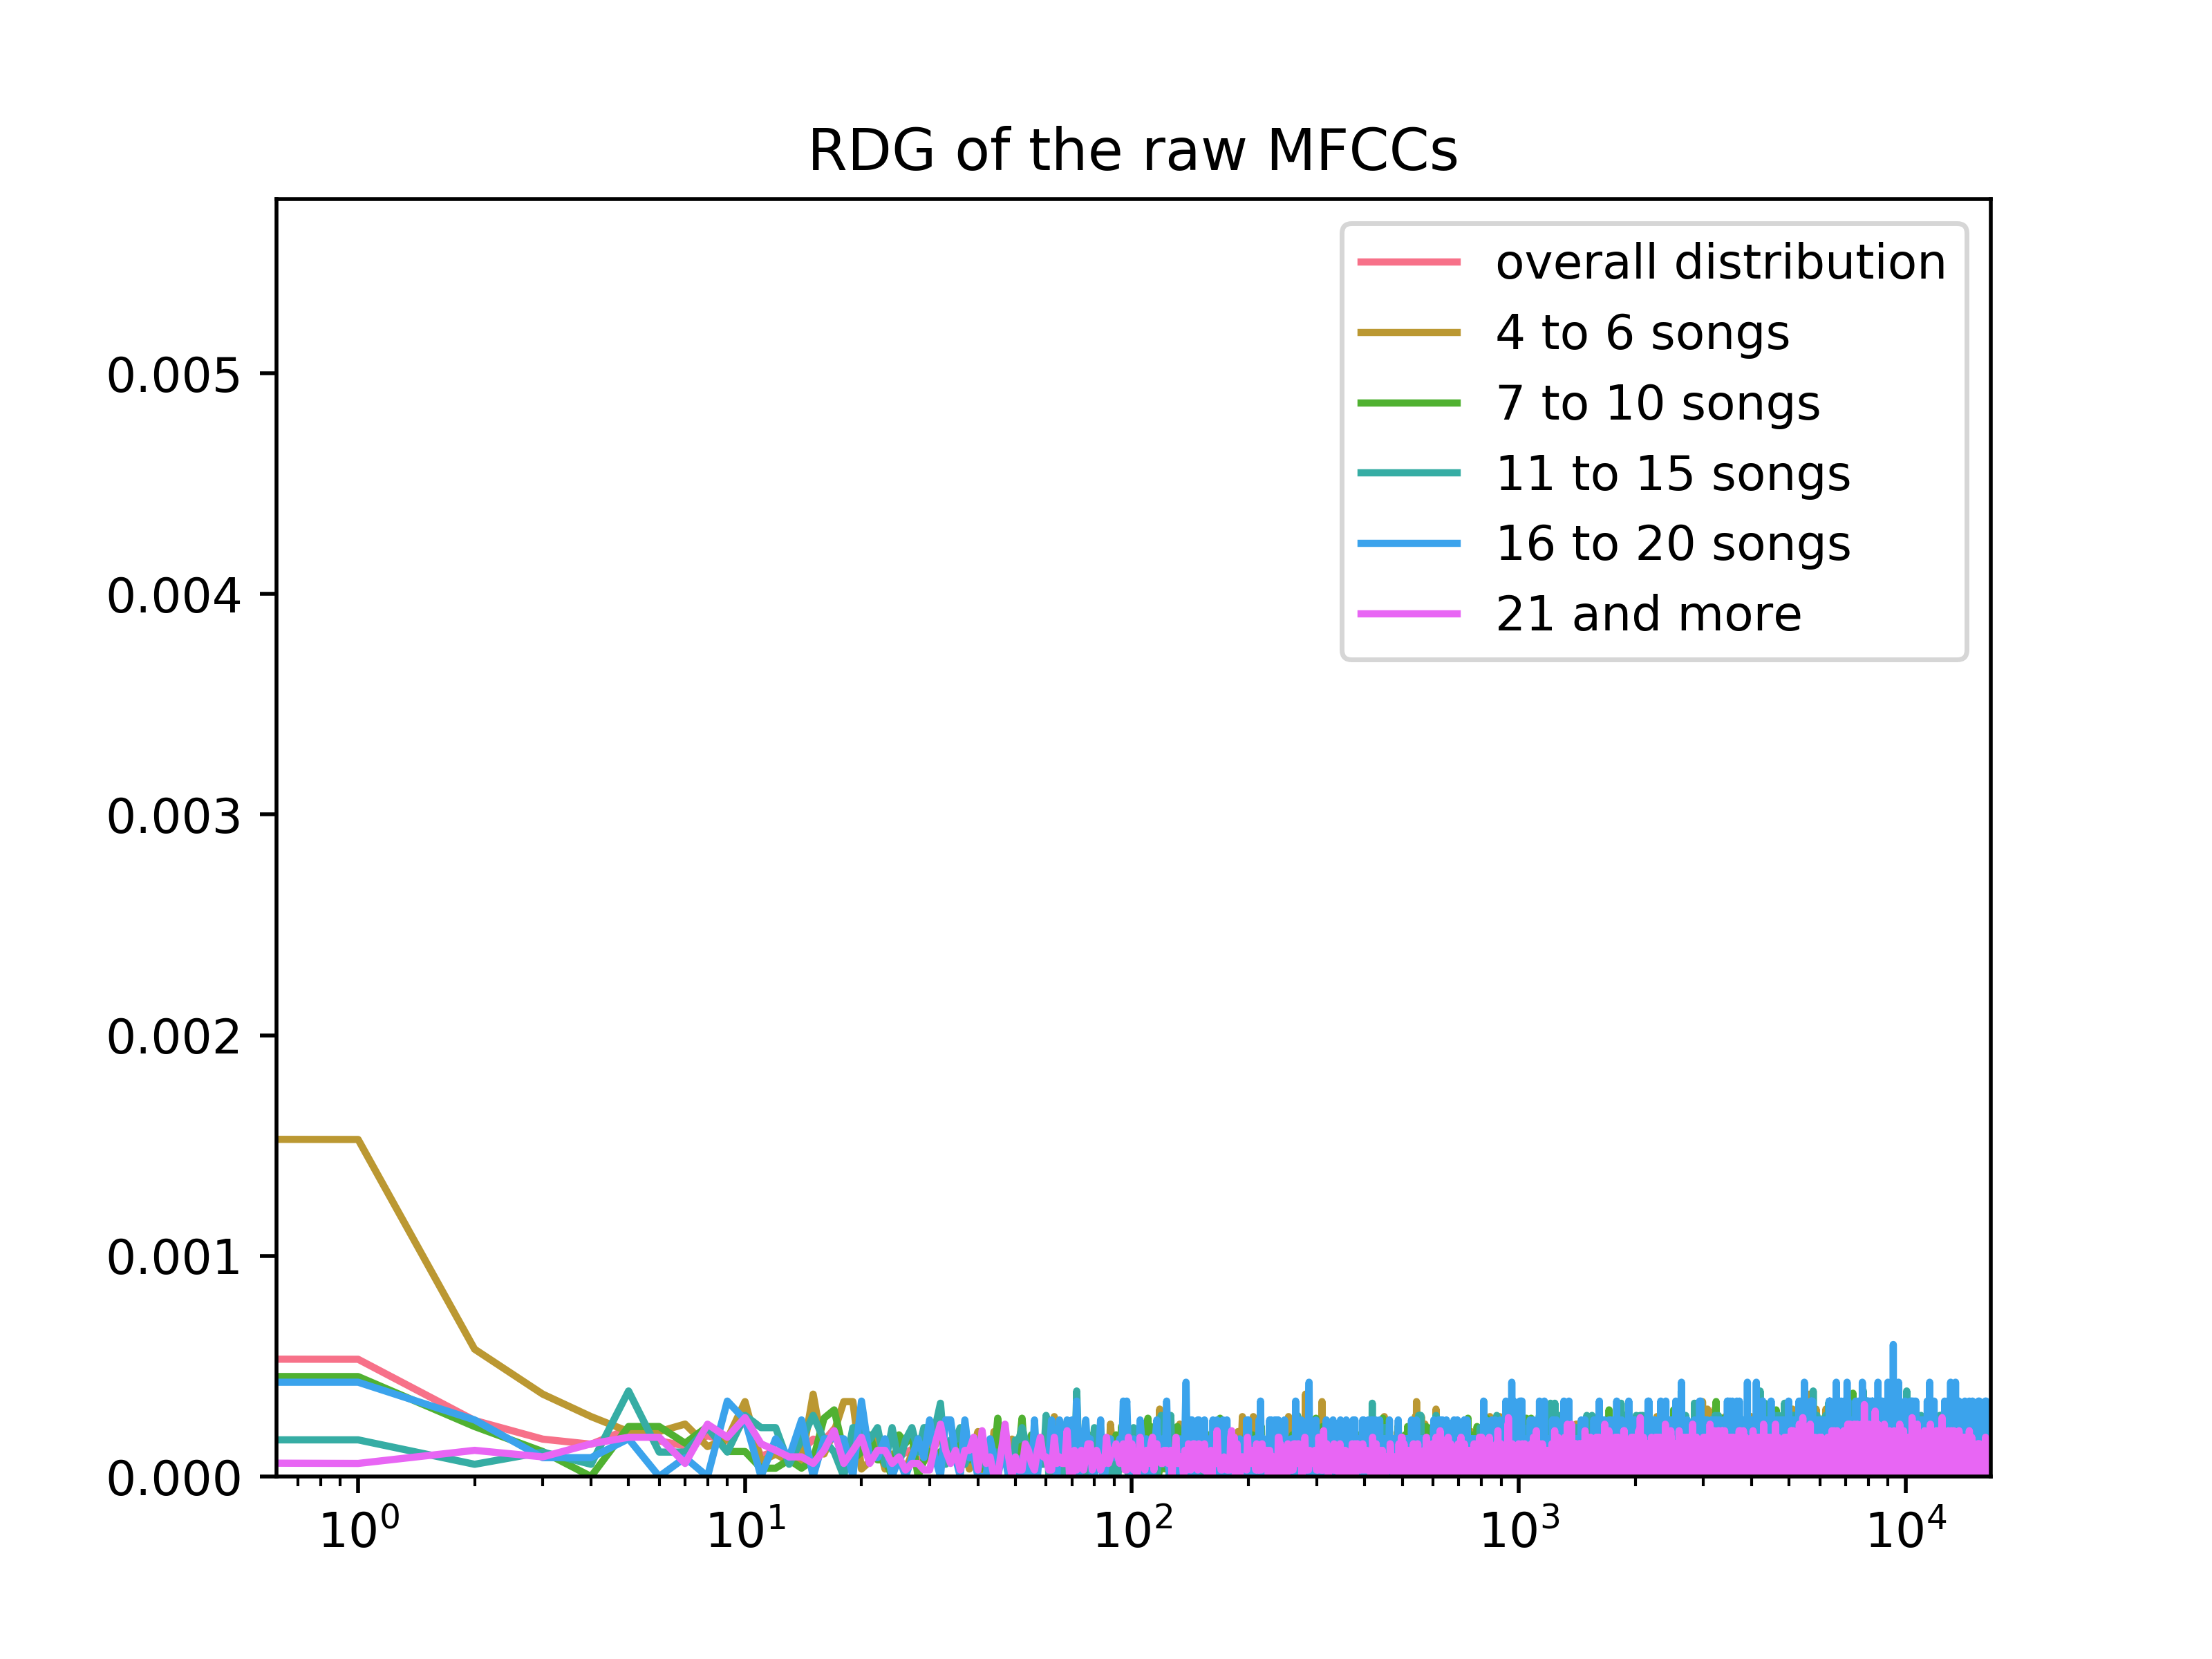
\includegraphics[width=120mm]{./img/mfcc_graph.png}
	\caption{Distribution of ranks of songs from the test set the MFCC method assigned them.}
	\label{fig:mfcc_graph}
\end{figure}


\subsection {PCA on spectrograms}

\subsubsection{Input}
We used spectrograms as described in \ref{ssec:audio_prep} as input for our PCA. Because the output of the \texttt{librosa.core.stft()} method is a complex matrix, we computed the absolute value for each matrix entry. Afterwards, we flattened the matrix into a single vector and normalized it. Normalization was very important, without it, the resulting rankings were almost random.

\subsubsection{Training}
Training proved to be a little bit challenging with input vectors of length 900048. As the whole (16594x900048) matrix did not fit into the PCA at once. So instead of using \texttt{sklearn.decomposition.PCA} we turned to a PCA with the possibility to train the PCA in batches. This kind of PCA is also provided by \textt{skearn} in the \texttt{sklearn.decomposition.incrementalPCA} module. \\ Our batch size was 1106. Again, when we tried to increase it, we got a memory error. This was a little inconvenient as for the PCA the maximum number of components is $min(n\_samples, n\_features)$. In our case, $n\_samples$ was only 1106 components which explained about 57\% of the dataset's variance.

\subsubsectio{Output}
Our output were vectors of length 1106 which we acquired when taking the trained incremental PCA model and calling \texttt{tranform()} with the spectrogram as a parameter.

\subsubsection{Results}

\begin{table}[h!]
\centering
\renewcommand{\arraystretch}{1.5}
\begin{tabu} to 1\textwidth { | c || c | c | c | c | c |}
 \hline
 \textbf{method} & \textbf{R@10} & \textbf{R@50} & \textbf{R@100} & \textbf{nGDC} & $ \boldsymbol{\overline{rank}} $ \\
 \hline
 \hline
 PCA\_spec\_1106 & 0.04317 & 0.05213 &  0.05945 & 0.03741 & 6729 \\
 \hline
 PCA\_spec\_320 & 0.03373 & 0.04392 &  0.05189 & 0.03209 & 6768 \\
 \hline
 GRU\_spec\_20400 & 0.00214 & 0.00563 & 0.00999 & 0.00356 & 7710 \\
 \hline
 GRU\_spec\_5712 & 0.00219 & 0.00616 & 0.01017 & 0.00370 & 7667 \\
 \hline
 LSTM\_spec\_20400 & 0.00924 & 0.01595 & 0.02214 & 0.01060 & 7601 \\
 \hline
 LSTM\_spec\_5712 & 0.00619 & 0.01244 & 0.01737 &  0.00744 & 7452 \\
 \hline
\end{tabu} \\
\caption{Table summarizing average rank values for all methods with spectrogram input averaged over the 5 cross validations}
\label{table:spec_methods}
\end{table}
 

\begin{figure}[h!]
\centering
\begin{minipage}{.5\textwidth}
  \centering
  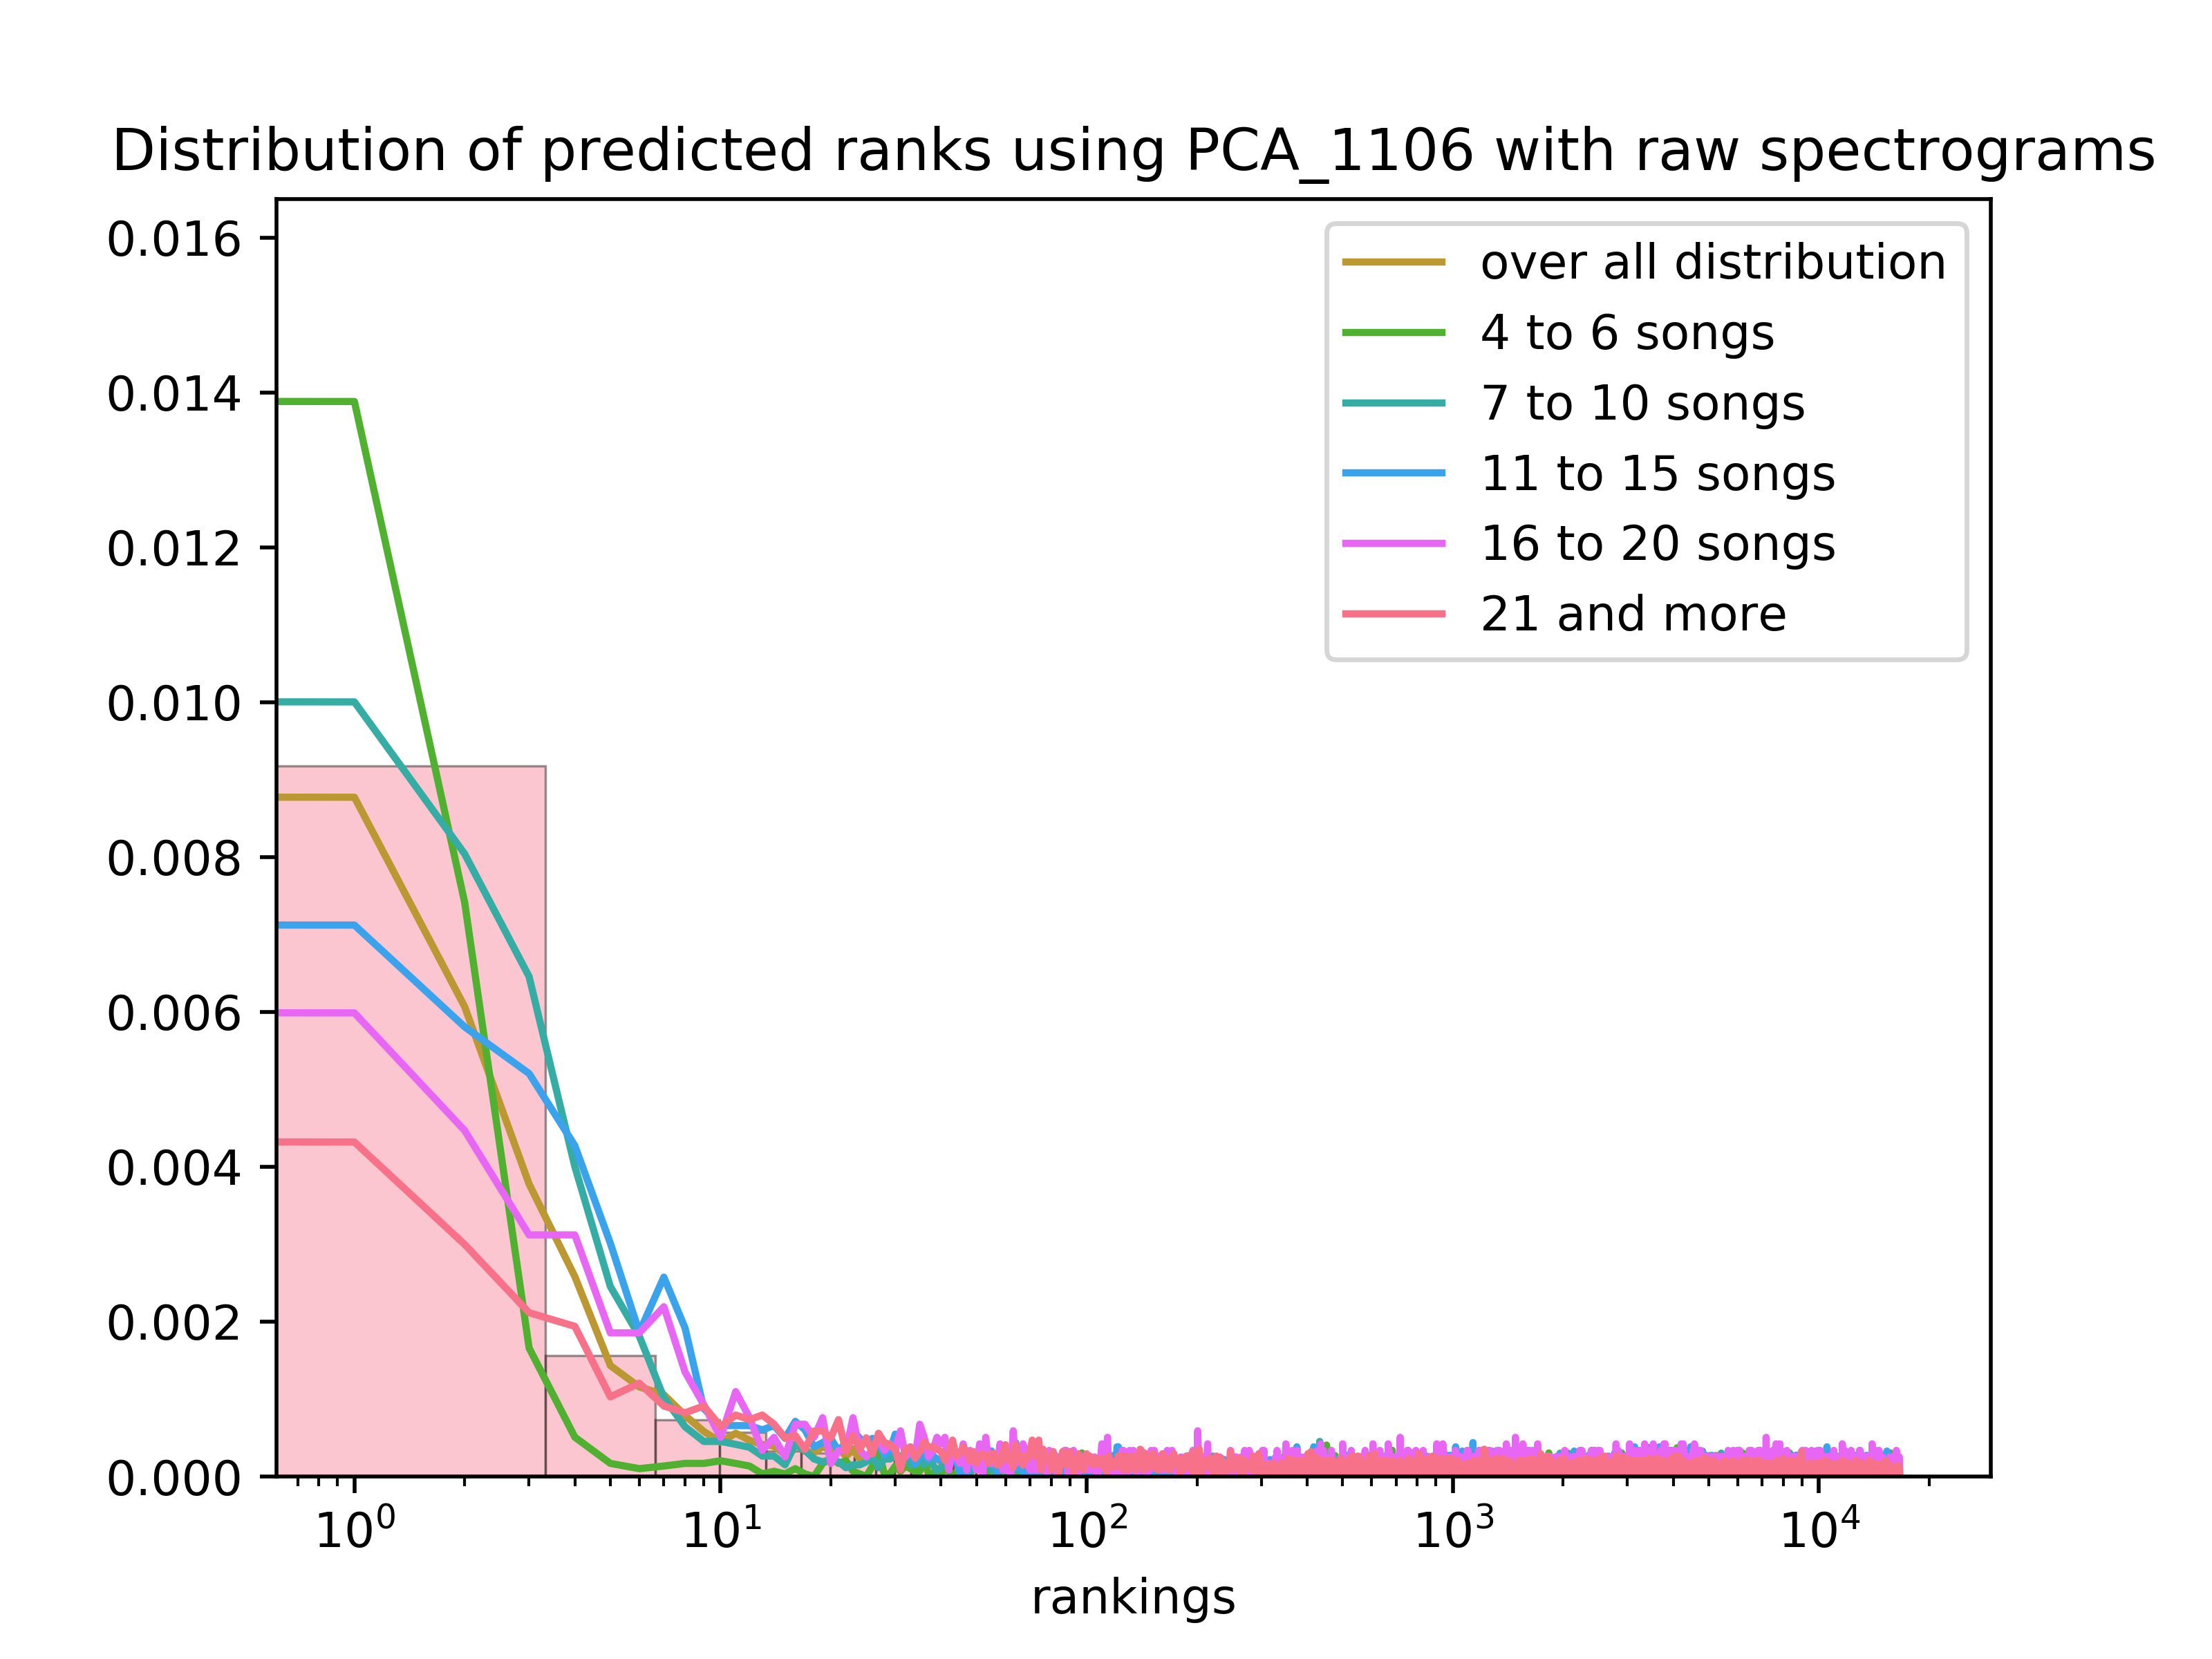
\includegraphics[width=1\linewidth]{./img/pca_spec_1106_graph.png}
  \captionof{Distribution of ranks of songs from the $p_{test}$ set the spectrograms method assigned them.}
  \label{fig:pca_spec_1106_distribution}
\end{minipage}%
\begin{minipage}{.5\textwidth}
  \centering
  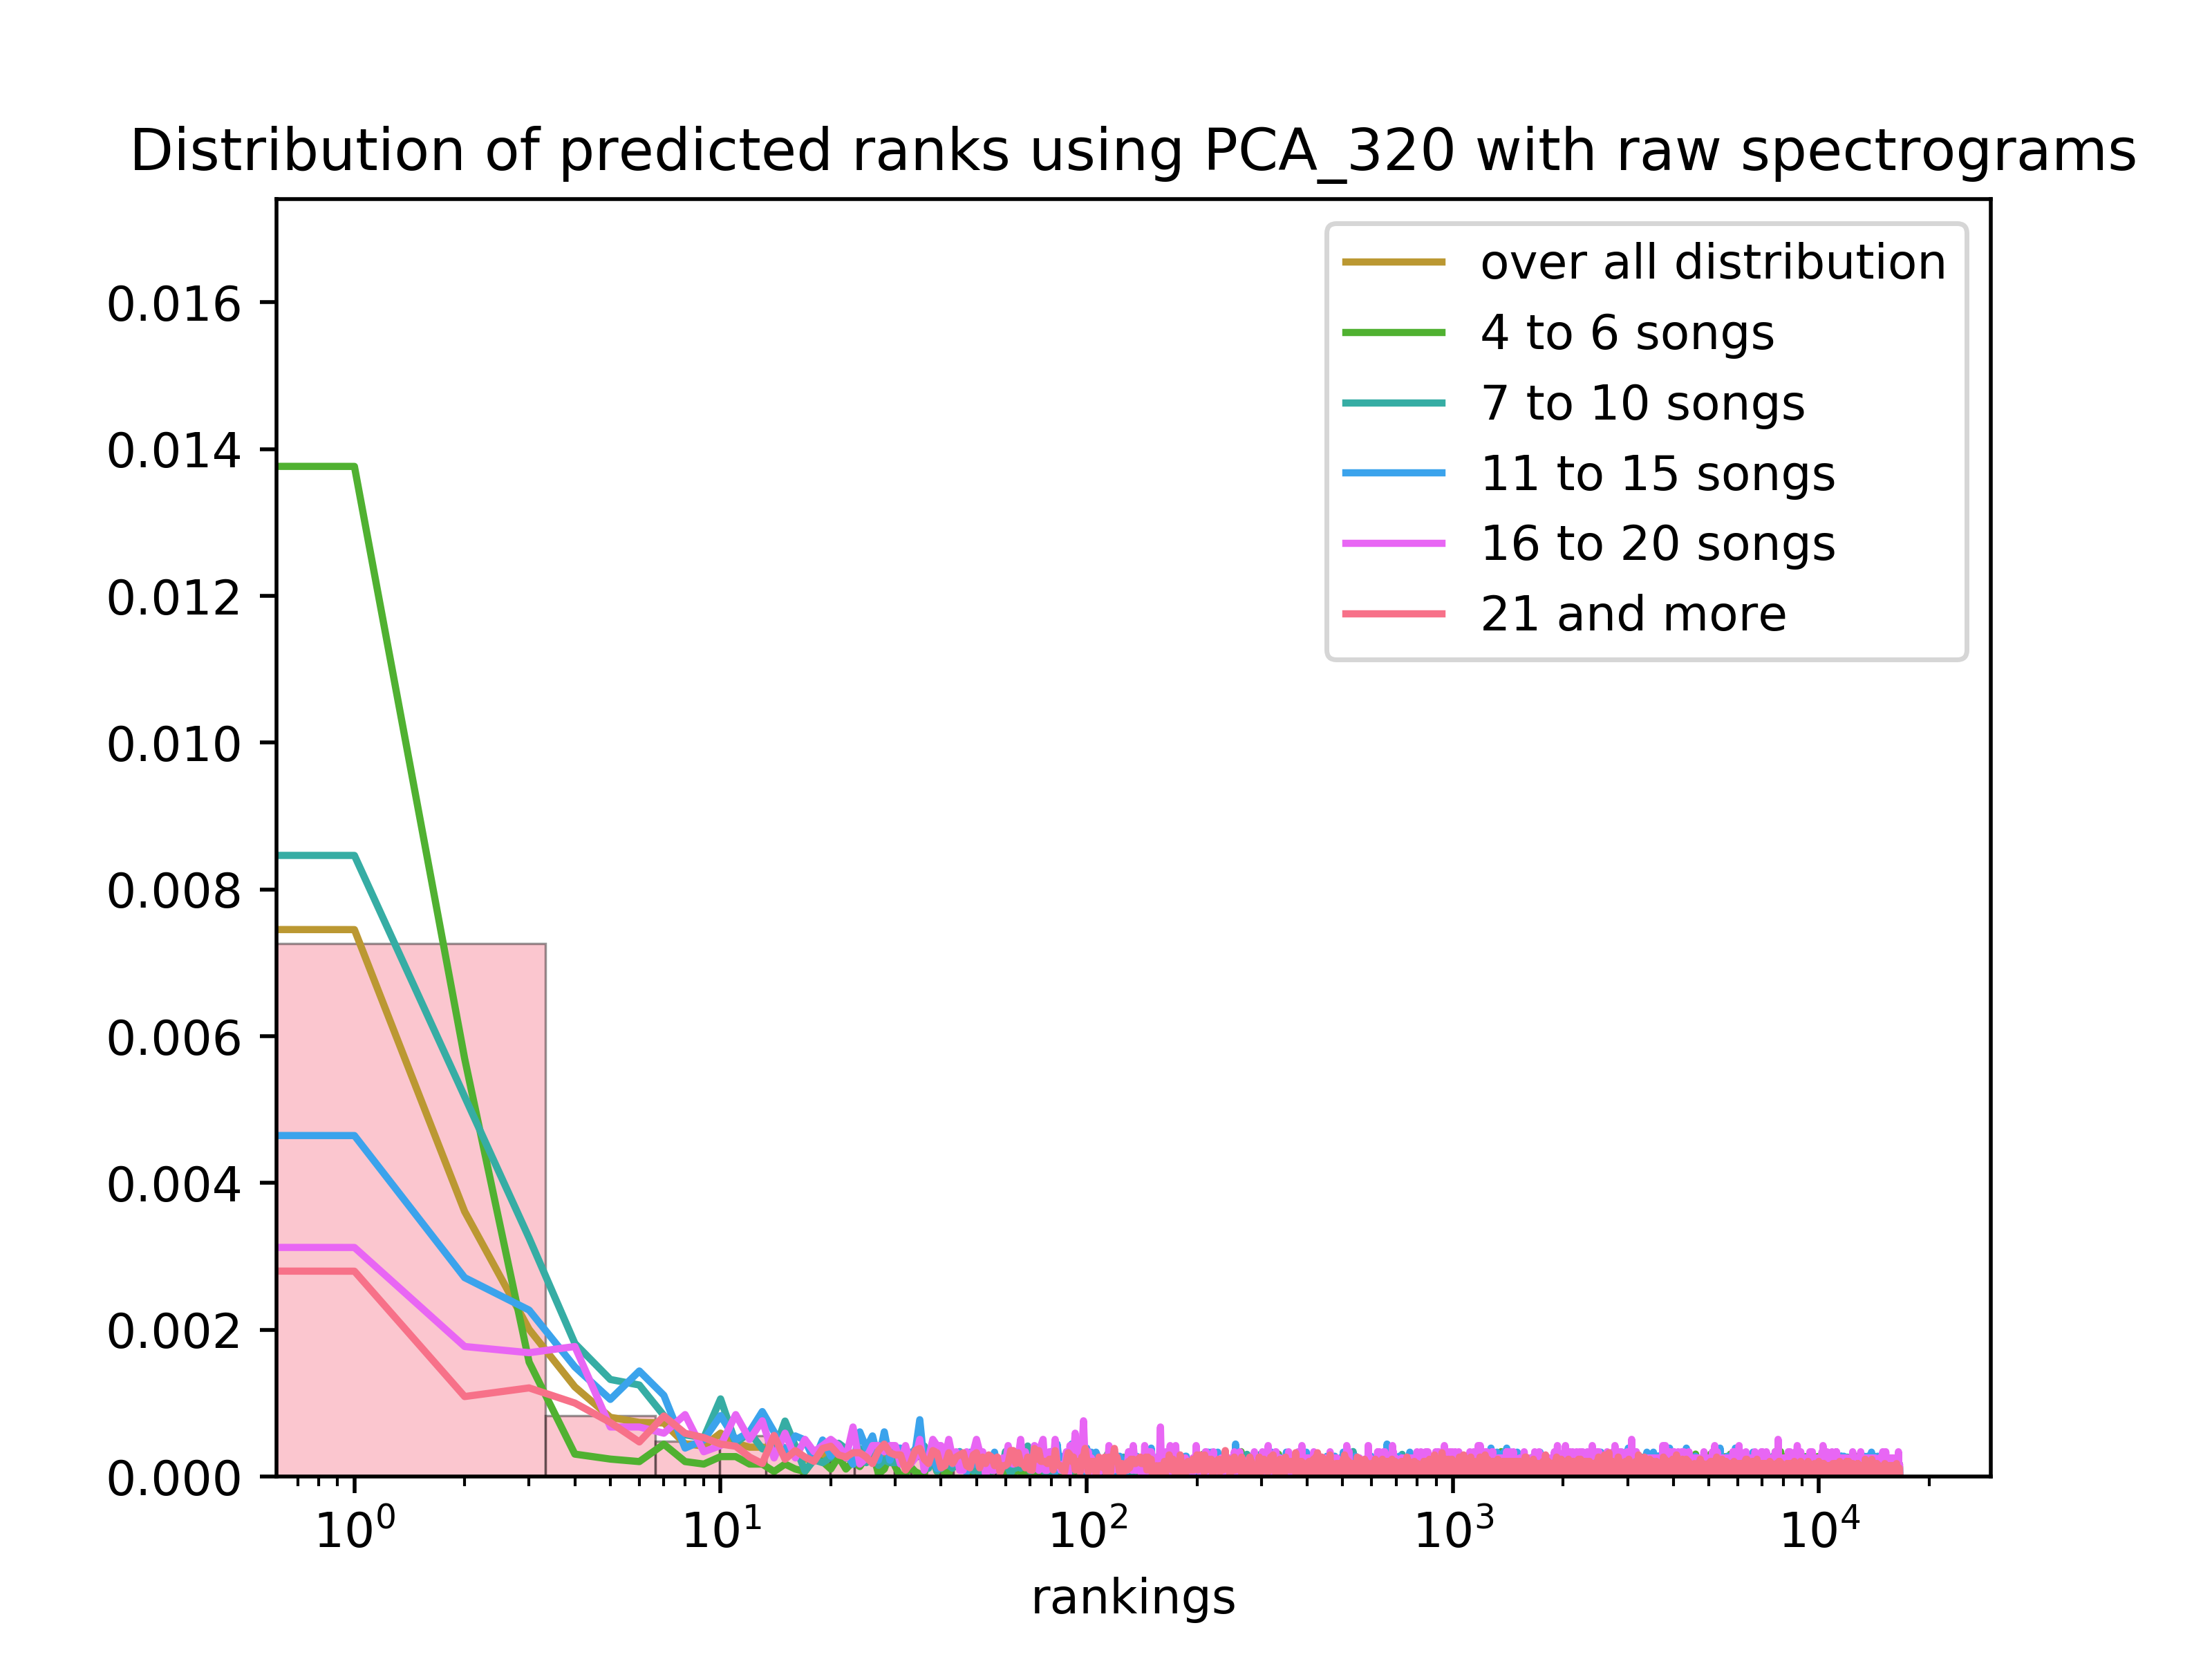
\includegraphics[width=1\linewidth]{./img/pca_spec_320_graph.png}
  \captionof{Distribution of ranks of songs from the $p_{test}$ for spectrograms vectors as input into PCA}
  \label{fig:pca_spec_320_distribution}
\end{minipage}
\end{figure}

The dimensionality reduction in this method was the biggest of all or our methods. Our song representation went from 900048 to 1106 dimensions. It seems though that even with only 57\% of explained variance this methods results were very good compared to other methods. \\
When seeing this, we decided to go for a even more radical reduction to vectors of length 320. This was inspired by the length of the W2V vectors. We called our bigger model $PCA_{1106}$ and our smaller model $PCA_{320}. $ The results of the smaller model were only slightly worse than those of the big one. This is especially interesting because the same tendencies were not observed in the case of PCAs with Mel-spectrogram inputs as will be illustrated later.

\subsection{PCA with Mel-spectrograms}
\subsubsection{Input}
The input for our Mel-PCA were mel-spectrograms from \ref{ssec:audio_prep} which were flattened and normalized using a \texttt{MinMaxScaler} from the \texttt{sklearn} Python package.

\subsubsection{Training}
Unlike with the spectrograms, mel-spectrograms fit into the memory so the PCA was able to train with the whole dataset at once. This allowed us again to find out what number of components explaines 90\% of the variance ratio and to use it. We found that 90\% of variance is explained by 5715 components which is also what we used to train our first model. \\
We were quite pleased by the results as it is the best method that we came up with. Therefore we were quite hopeful when reducing the dimension even more to 320 as we did with PCA on spectrograms. We again created two models, one is called the $Mel\_PCA_{5715}$ the other the $Mel\_PCA_{320}$. 

\subsubsection{Output}
Our output for the bigger model was a vector of length 5715, for the smaller model, it was a vector of length 320.

\subsubsection{Results}
To our disappointment, the more radical dimension reduction did not improve the performance of the PCA\_mel method. It actually worsened the results significantly as can be observed in Table \ref{table:mel_spec_methods}. 

The \ref{fig:pca_mel_comparison_graps} illustrates the immense performance drop between a PCA\_mel\_5715 components and a PCA\_mel\_320. Another thing to notice here though which only applies to the Mel\_PCA\_{5715} is that the drop of top rankings for longer playlists is not quite significant compared to all the other methods we tested. We still observe the trend of worse results for longer playlists, however, it is not as significant compared to for example the the method with raw Mel-spectrograms.
\begin{figure}[h!]
\centering
\begin{minipage}{.5\textwidth}
  \centering
  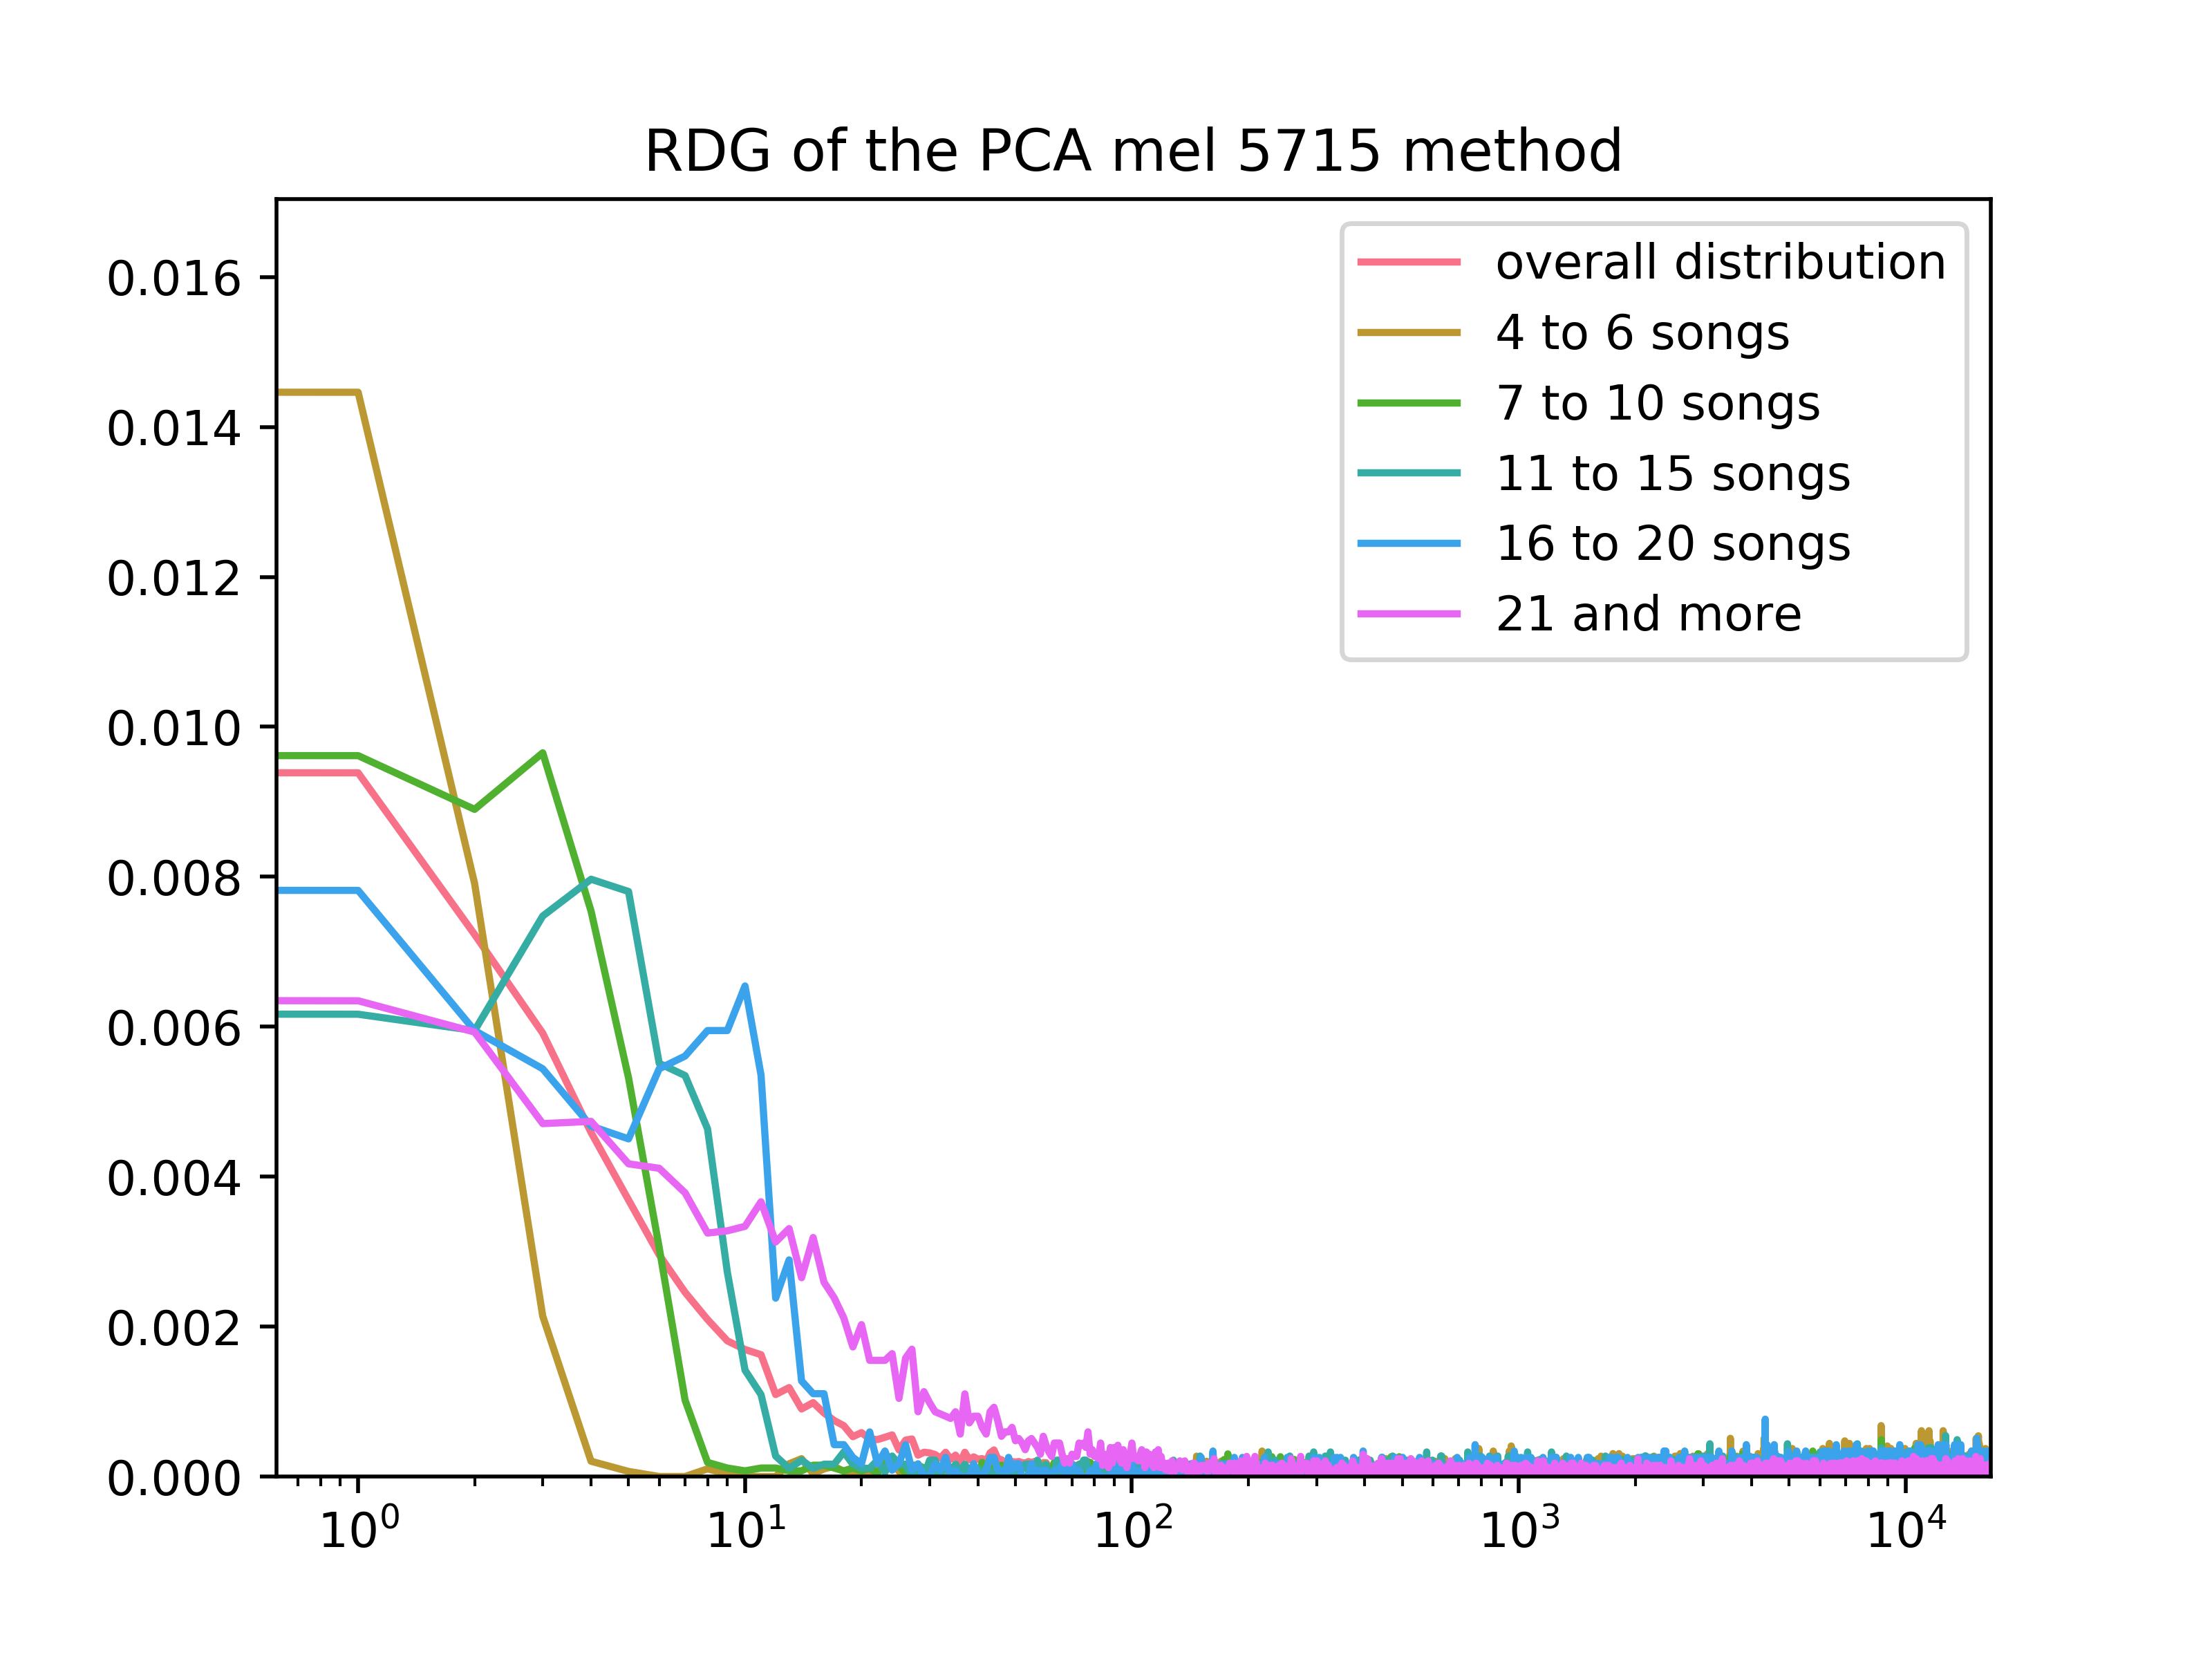
\includegraphics[width=1\linewidth]{./img/pca_mel_5715_graph.png}
  \captionof{Distribution of ranks of songs from the $p_{test}$ set the spectrogram method assigned them.}
  \label{fig:pca_mel_5715_distribution}
\end{minipage}%
\begin{minipage}{.5\textwidth}
  \centering
  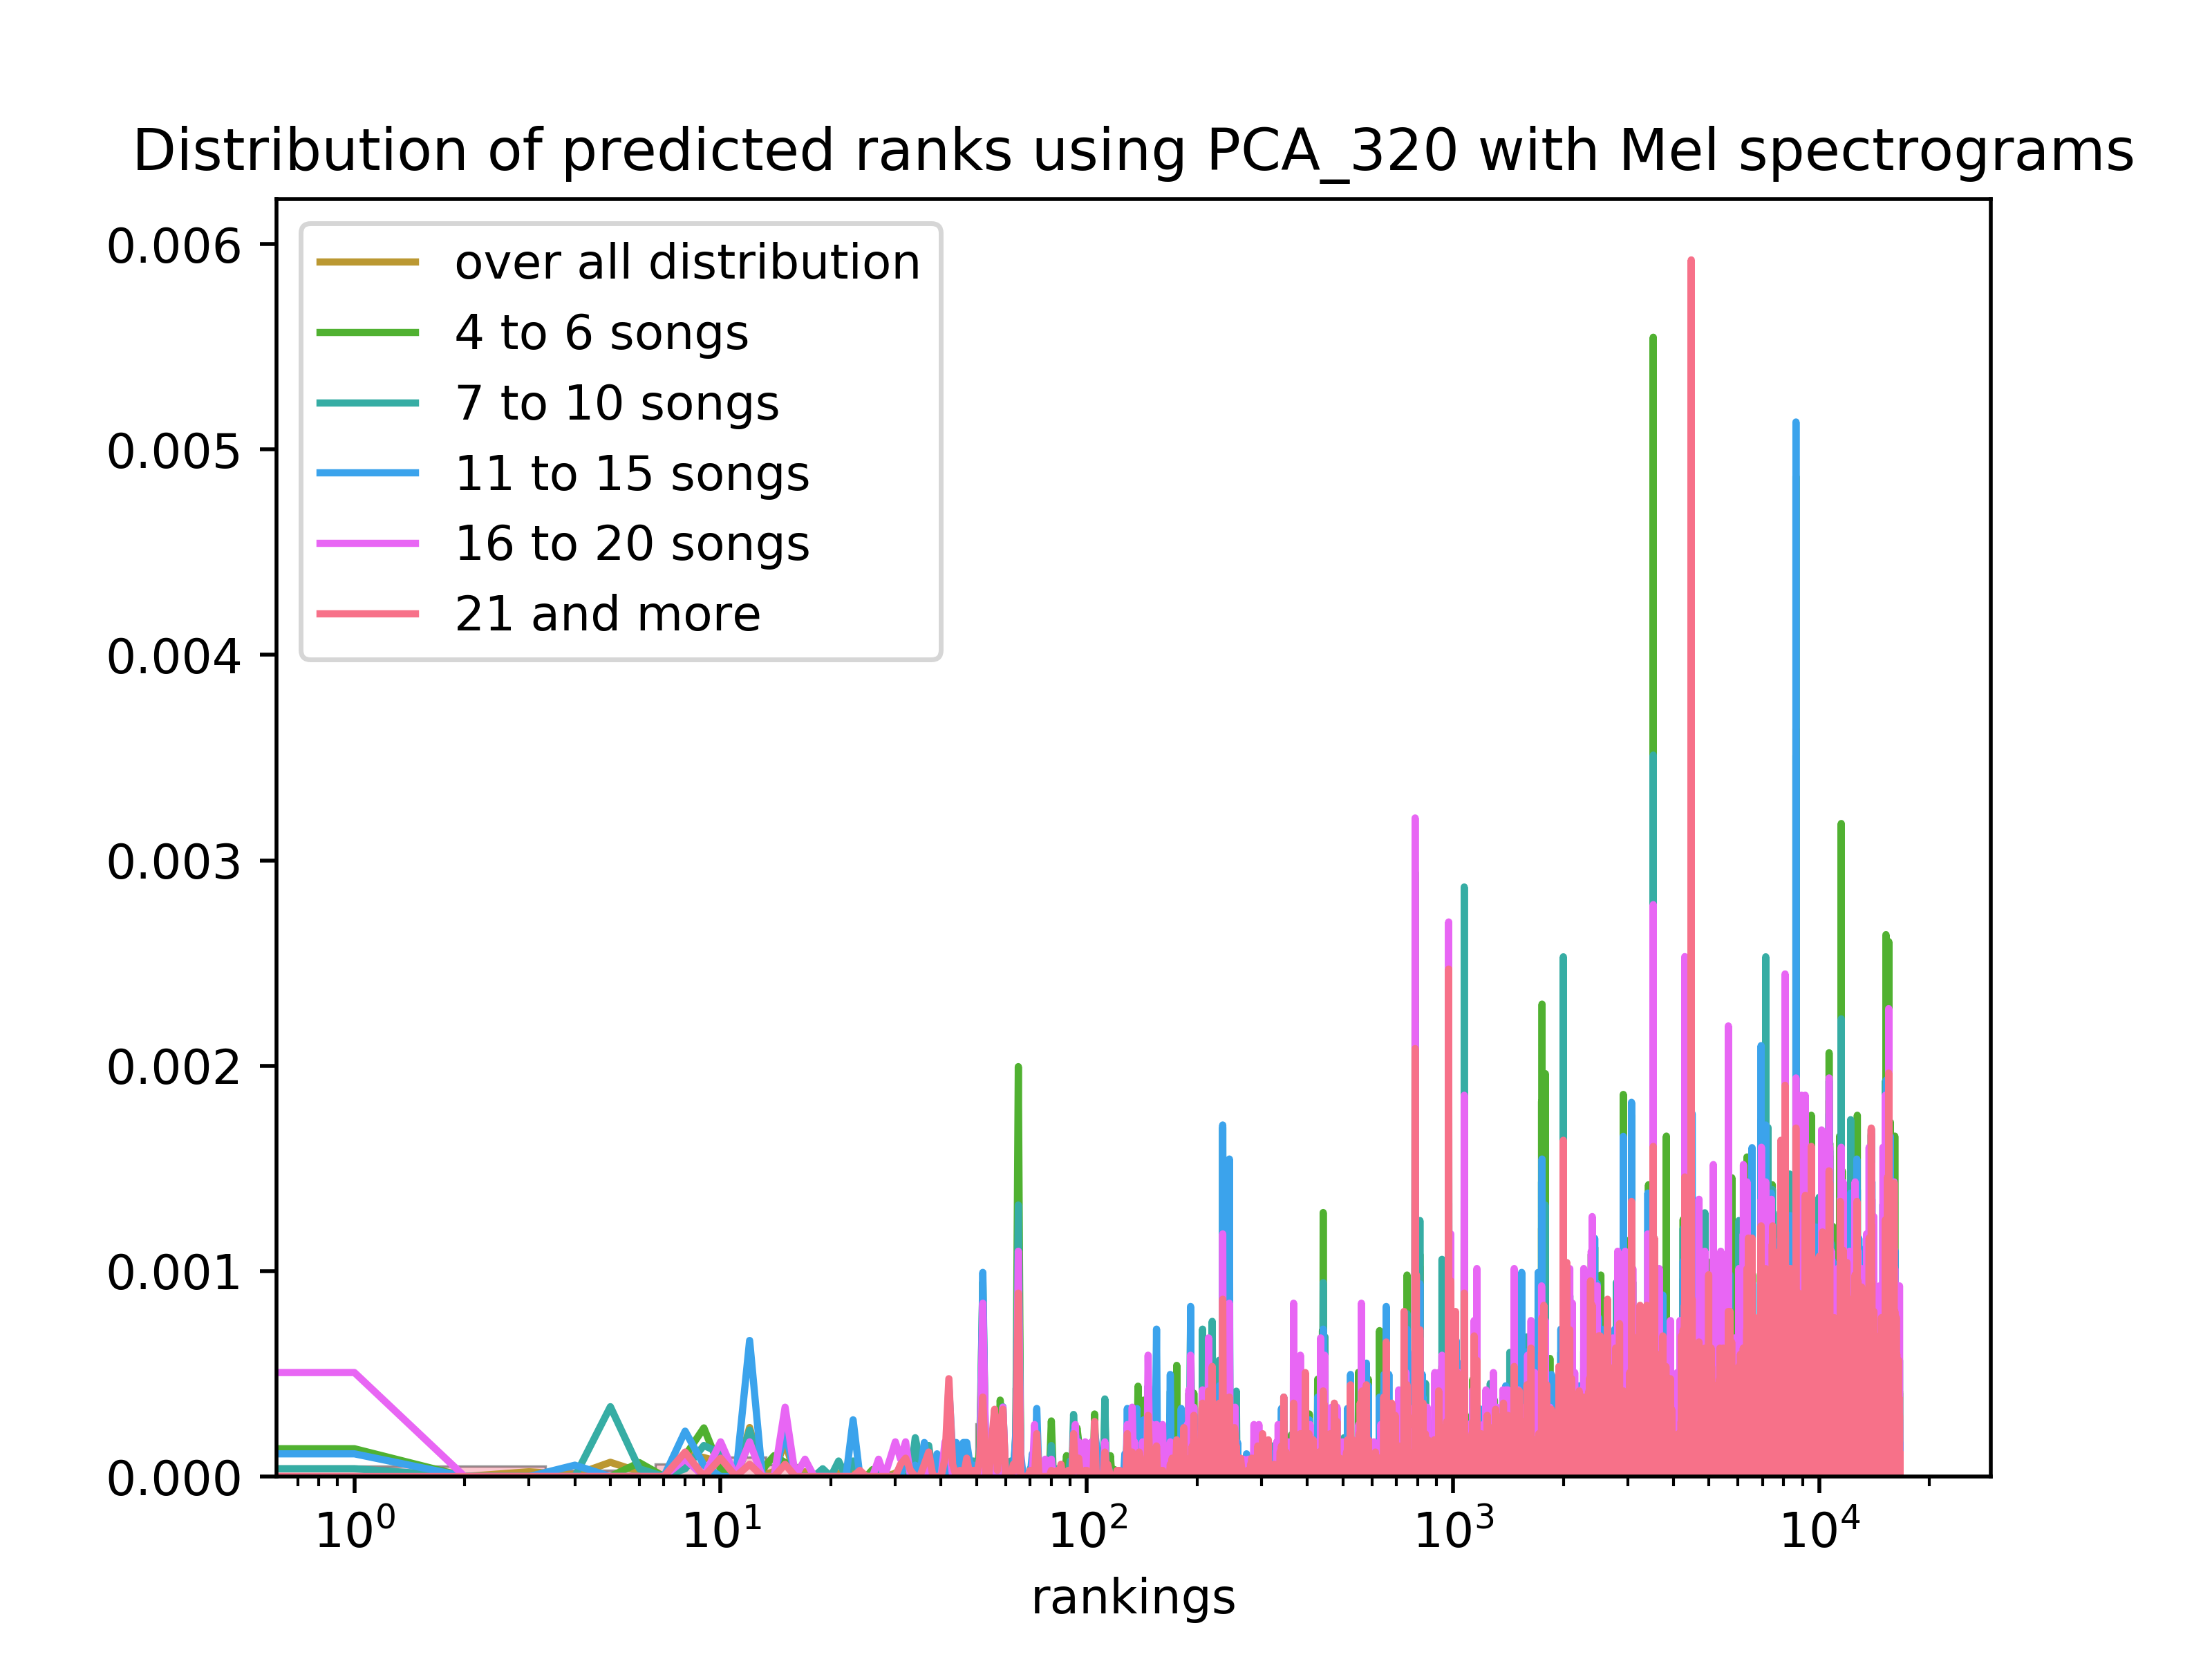
\includegraphics[width=1\linewidth]{./img/pca_mel_320_graph.png}
  \captionof{Distribution of ranks of songs from the $p_{test}$ for spectrogram vectors as input into PCA}
  \label{fig:pca_mel_320_distribution}
\end{minipage}
\end{figure}\label{fig:pca_mel_comparison_graps}

\section{Deep audio experiments}

\subsubsection{Architecture}
Before analysing each or the audio method using deep neural networks independently we will describe the two architectures we used. \\

As stated multiple times before, we decided to build our network based on the \cite{inproceedings_RNNs} paper. We chose our audio extraction coefficient based on their findings and we also designed our architecture in a way they did with some slight adjustments and extensions. \\

The first most notable thing is, that their network was designed to classify sounds, not encode songs. One might think that this would make their RNN unsuitable for our task, and it did as a whole. However their network consisted of two parts. The first part was an autoencoder and the second part a multi-layer perceptron. The autoencoder was trained in an unsupervised manner and the outputs were then fed into the MLP which did the classification. \\

For the purposes of our work, we only used the autoencoder part. Unlike them, instead of using the \texttt{auDeep} library we decided to build our networks with the \texttt{Keras} library \cite{chollet2015keras} as it has a user-friendly model creation API. We had also access to GPU computers and \texttt{Keras} (in our case with the \texttt{Tensorflow} backend) makes it easy to train networks faster with the access to GPUs. \\

We created two architectures. One with two GRU layers at the beginning as the encoder and one Bidirectional layer as the decoder. This follows the paper. We also decided to create another architecture with LSTM layers instead of GRU layers even though \citeauthor{inproceedings_RNNs} found in their work that the additional complexity did not yield better results. Both architectures can be seen in Figure \ref{fig:nn_architectures} \\

\begin{figure}[h!]
\centering
\begin{minipage}{.5\textwidth}
  \centering
  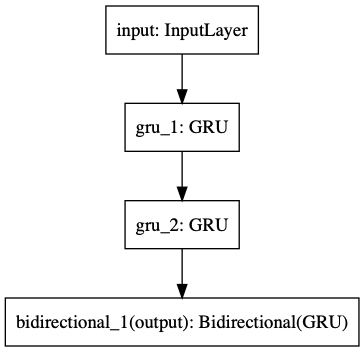
\includegraphics[width=1\linewidth]{./img/gru_architecture.png}
  \captionof{The general architecture of our GRU neural networks}
  \label{fig:gru_architecture}
\end{minipage}%
\begin{minipage}{.5\textwidth}
  \centering
  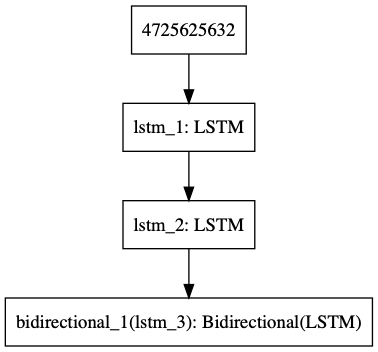
\includegraphics[width=1\linewidth]{./img/lstm_architecture.png}
  \captionof{The general architecture of our LSTM neural networks}
  \label{fig:lstm_architecture}
\end{minipage}
\end{figure}\label{fig:nn_architectures}


The main motivation behind using LSTMs as well as GRU layers in our thesis was that LSTM layers are specifically suited for sequential data such as audio. GRU layers are a simplified version of LSTMs. We were hoping that the more complex layers could encode our audio data into the same dimensions as the GRU networks but help to make the similarities more accurate. \\

We used the \textit{mean squared error} as our loss function which is the standard for autoencoder networks. Our optimiser was \textit{adam} the same as in the \cite{inproceedings_RNNs} paper. We had to decrease the learning rate from 0.001 to 0.0001. Before we did that, our resulting predicted vectors often consisted of just \textit{NaN}s.

\subsubsection{Inputs and outputs}
Both the GRU and the LSTM network had three kinds of inputs --- the spectrograms, mel-spectrograms and the MFCCs. They were all passed in the form of 2D matrices containing $(n\_features, n\_timestamps)$. GRU as well as LSTM networks take 2D matrices and not just 1D vectors as input. Before training, the inputs were normalized using the \texttt{MinMaxScaler} with values between 0 and 1. \\
One important thing to note here is that these kind of networks that process sequential data in the form of 2D matrices reduce the dimensionality of only the $n\_features$ and not the $n_{timestamps}$. Our 15 second audios yielded 408 time stamps and 2206 features for spectrograms and 408 time stamps and 320 features for mel-spectrograms. With MFCCs the number of time stamps was 646 and the number of features 128. Therefore we did not attempt a dimensionality reduction as big as with PCA which does not care if a feature is a time stamp or a sample.

\subsection{GRU network with spectrogram input}

\subsubsection{Training}

We trained two GRU spectrogram networks with variable output vector lengths. We decided to base our vector length on the PCA explained variance ratio. For spectrograms however, we only found out that 1106 explains 56\%of variance. Therefore, we took the information from the mel-spectrogram PCA where 5715 explains 90\% of variance and did a simple calculation $$ l(mel\_spec_{transformed})/l(mel\_spec) = l(spec_{transformed})/l(spec) $$. To keep the proportional reduction same as for mel-spectrograms and the output length of 5715 where $l(x)$ is the length of either the spectrogram or mel-spectrogram flattened. This would mean an output vector length of almost 40000. We decided that it would be too much for any practical use in our web application and reduced it to 20400 which at that point we thought could be potentially used. The shorter vectors used as encodings of our spectrograms were of length 5712. This inspired by the Mel-spectrogram PCA as we thought that the neural network could mimic the Mel-frequency reduction as well as additional reduction. \\
In our base paper, they trained their autoencoders for 50 epochs using batch sizes of 64. We found this to be insufficient especially with our learning rate reduction. For GRU networks with spectrograms we set the number of epochs to 100 and the batch size to 295 (for higher batch values we got memory errors). 

\subsubsectiom{Results}
As can be observed in Figure \ref{fig:all_model_training} the loss is basically constant for both GRU networks with spectrogram input (the GRU\_spec\_20400 is hidden behind the orange line of GRU\_spec\_5712 as their progress or rather the lack of it is the same). This means, that the network did not really improve for some reason. Therefore it is not suprising that the results of this method are not between our best ones.

We can see in Table \ref{table:spec_methods} that only 0.2\% of songs was ranked in the top 10, 0.5\% in the top 50 and 1\% in the top 100 for the longer GRU spectrogram model. For the short GRU spectrogram model, the results are a slightly better with 0.2\% for the top ten songs 0.6\% ranked in the top 50 and a little over 1\% ranked in the top 100. The ranking improvement is just very small and almost non-existent when rounding the numbers to two decimal places and then converting them into percentages. \\
The distributions depicted in Figure \ref{fig:gru_spec_distributions} of both GRU\_specs is are similar too. The trend for worse ranks for songs from longer playlists is apparent in both method graphs but it is not as obvious as in methods that have over all better results.

\begin{figure}[h!]
\centering
\begin{minipage}{.5\textwidth}
  \centering
  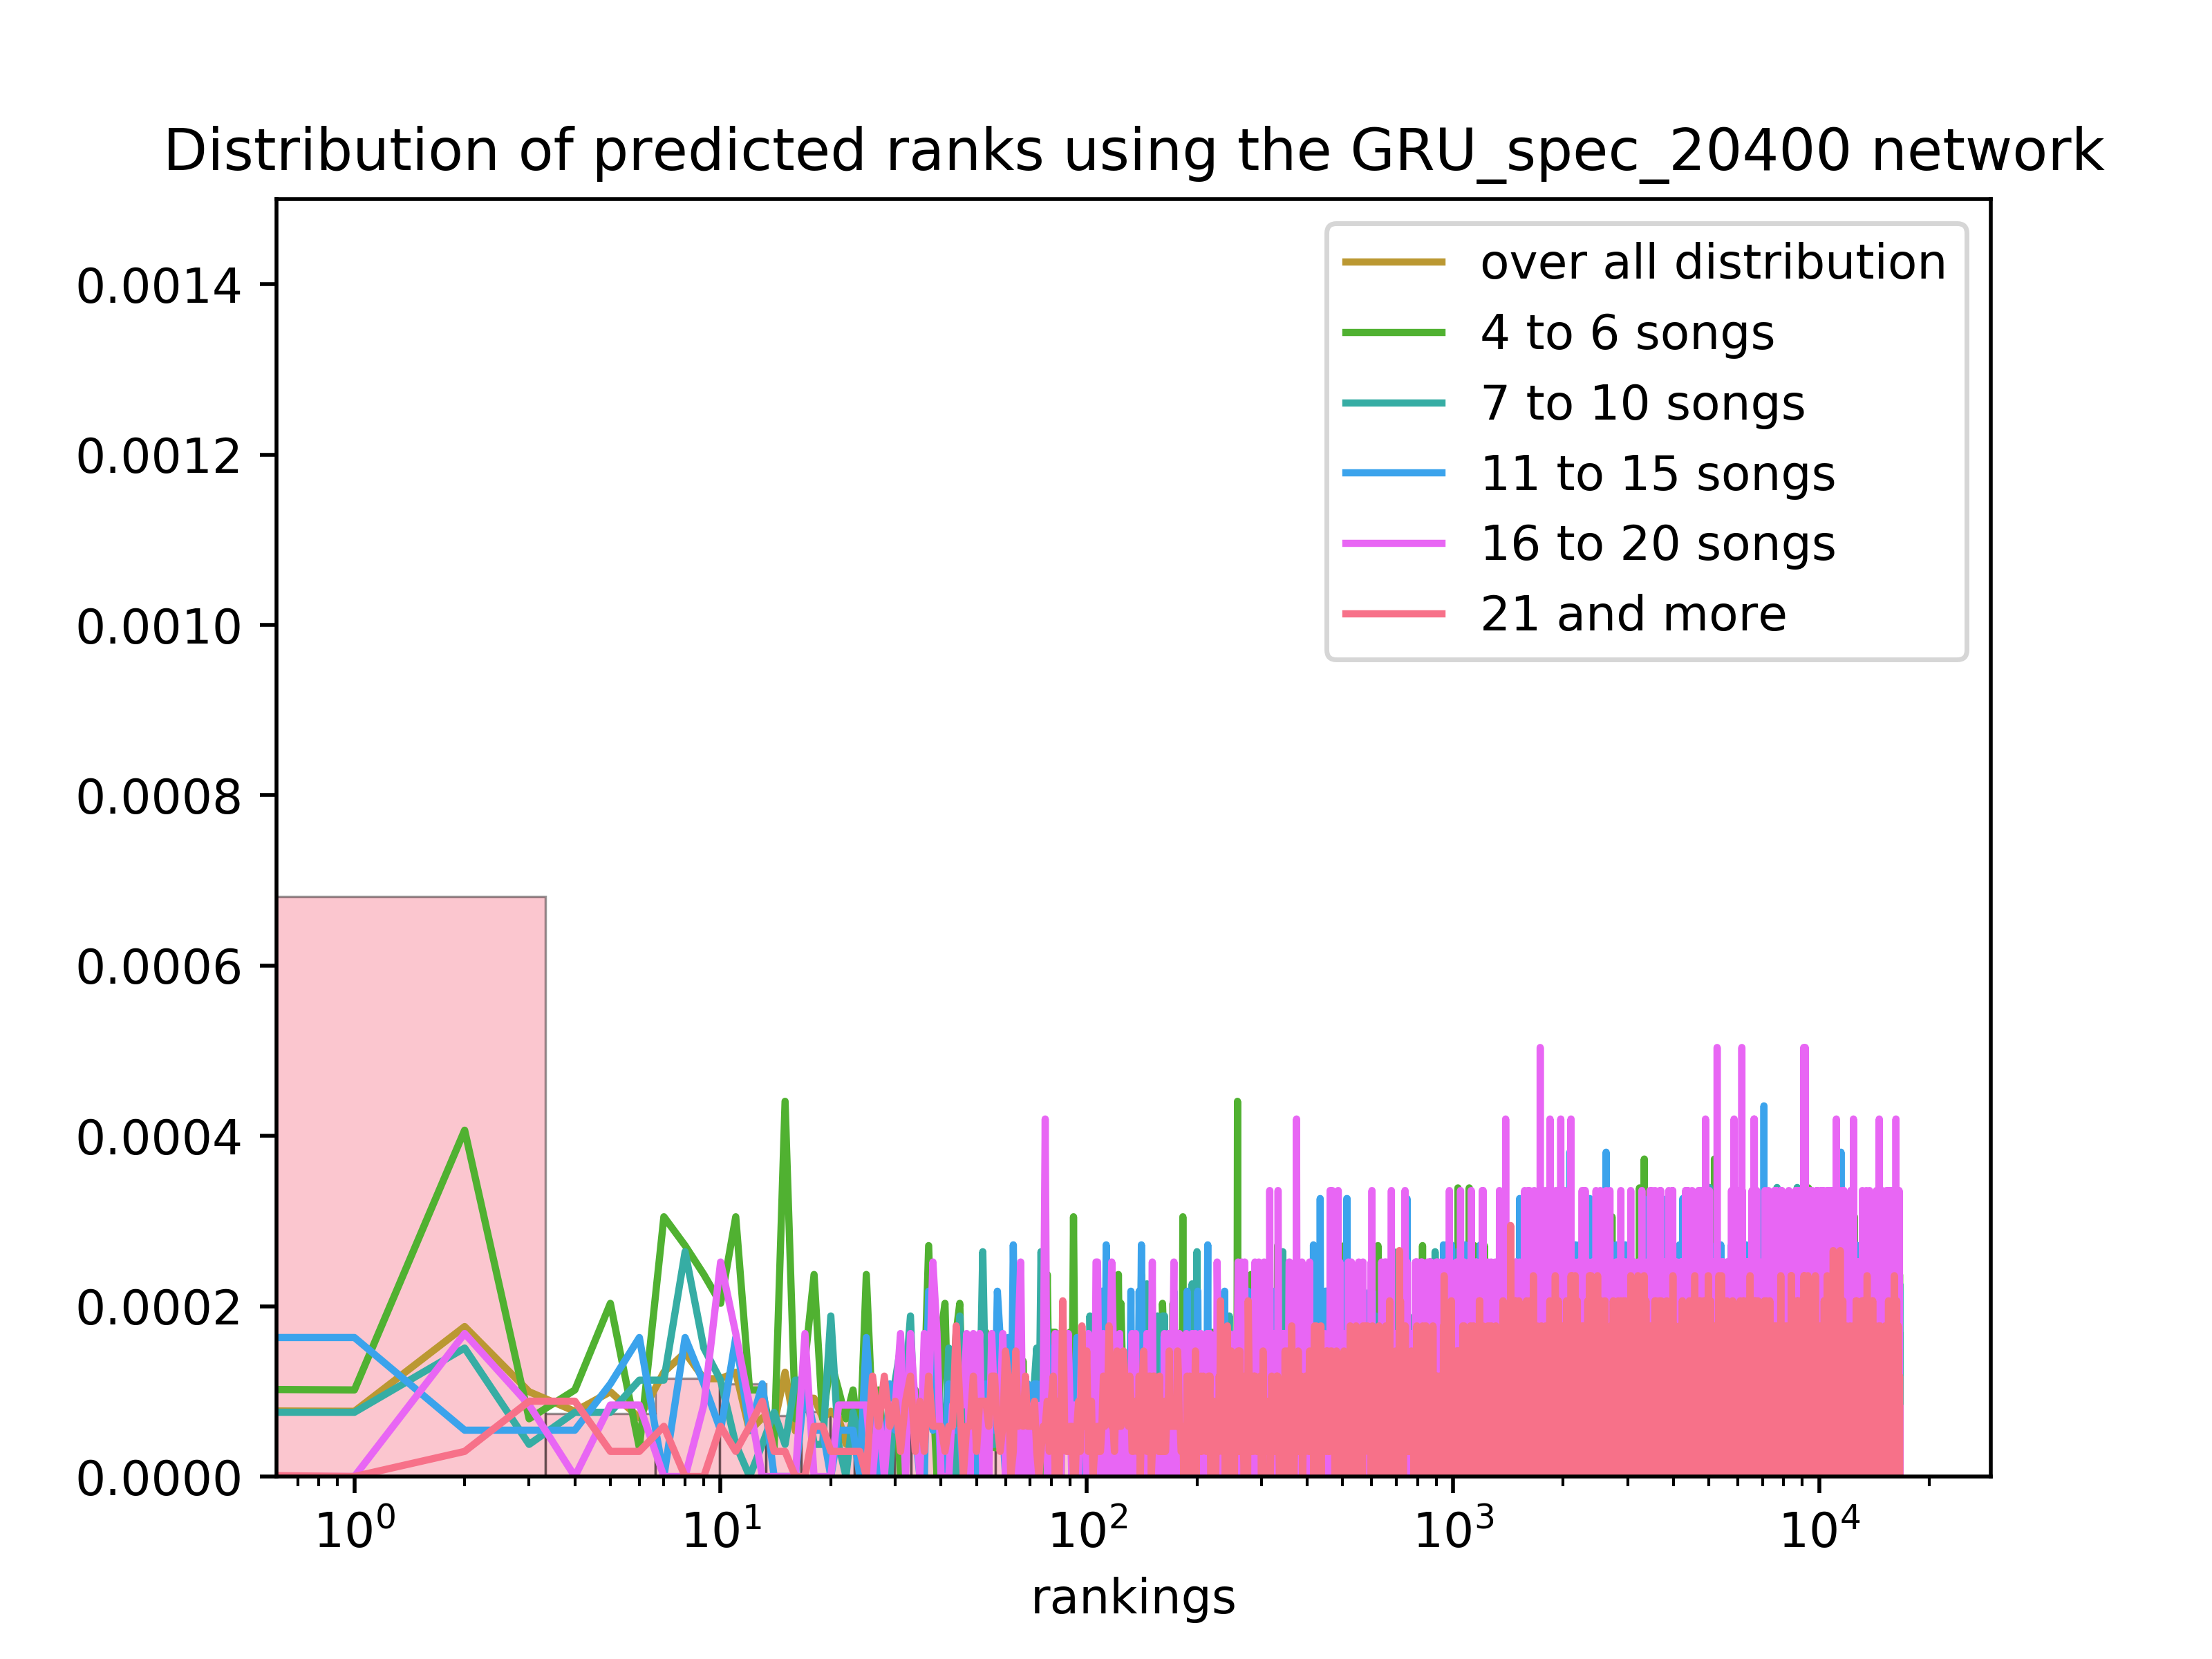
\includegraphics[width=1\linewidth]{./img/gru_spec_20400_graph.png}
  \captionof{The distribution of predicted ranks using the long GRU spec encodings.}
  \label{fig:gru_spec_20400_distribution}
\end{minipage}%
\begin{minipage}{.5\textwidth}
  \centering
  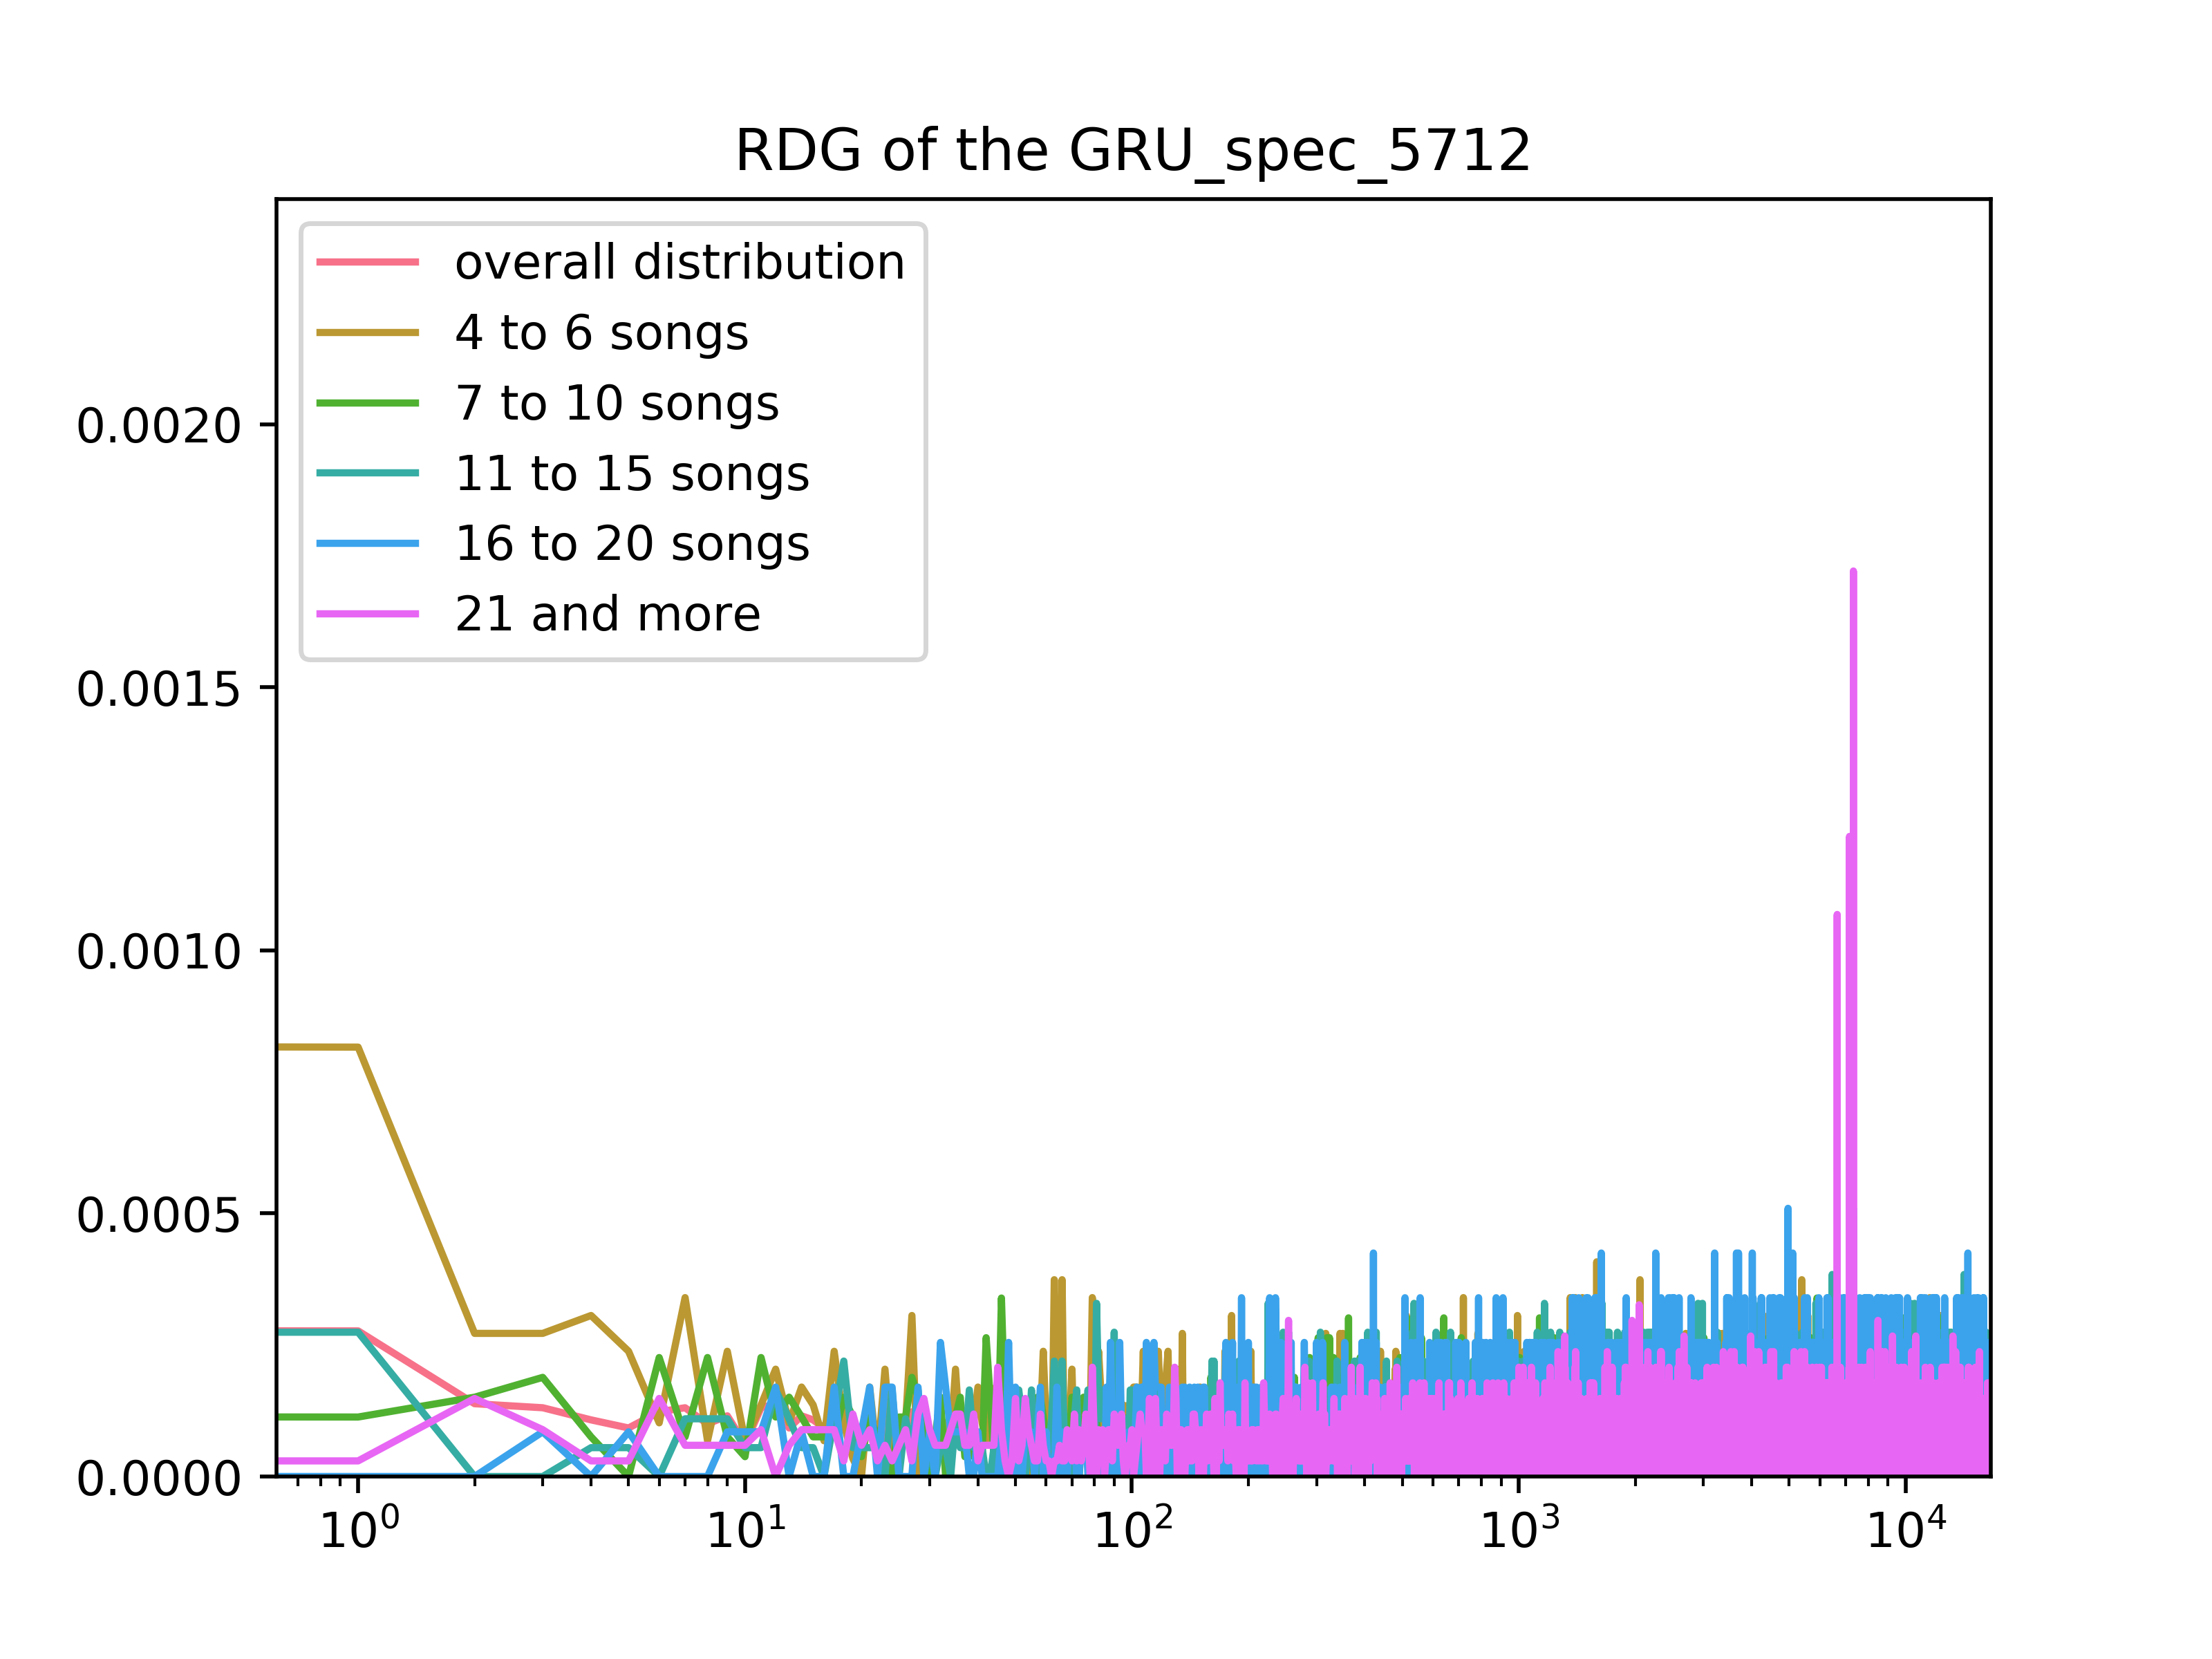
\includegraphics[width=1\linewidth]{./img/gru_spec_5712_graph.png}
  \captionof{The distribution of predicted ranks using the short GRU spec encodings.}
  \label{fig:gru_spec_5712_distribution}
\end{minipage}
\end{figure}\label{fig:gru_spec_distributions}

\subsection{LSTM network with spectrogram input}

\subsubsection{Training}
We chose the same training strategy for LSTMs with spectrogram input as we did for the GRU\_spec networks. It makes the comparison of both methods more fair under the same conditions. We also created two versions of our LSTM models, one LSMT\_spec\_20400 and the shorter version LSTM\_spec\_5712. The lengths are the same as with GRU\_specs and the motivation behind them is identical.

\subsubsection{Results}
Unlike the GRU model training which showed almost no improvement even after 100 epochs of training, our LSTM\_specs as one can observe in Figure \ref{fig:all_model_training} where the LSTM\_spec\_20400 is rendered in green and the LSTM\_spec\_5712 in red went through at least some progress. The decrease of loss slowed down significantly towards the end of the 100 epochs. \\
The higher training improvement correlates with better results for the LSTM\_spec methods. In Table \ref{table:spec_methods} are both the results of the LSTM\_spec models. They are better than those of the GRU\_spec models. \\
A thing worth noting here is that with the shorter encoding vector the results worsened. Definitely more dramatically than how the GRU\_spec results imporoved. The values in Table \ref{table:spec_methods} and distribution in Figure \ref{fig:lstm_spec_distributions} visualize the difference clearly, especially when it comes to songs from short playlists where the difference most apparent.

\begin{figure}[h!]
\centering
\begin{minipage}{.5\textwidth}
  \centering
  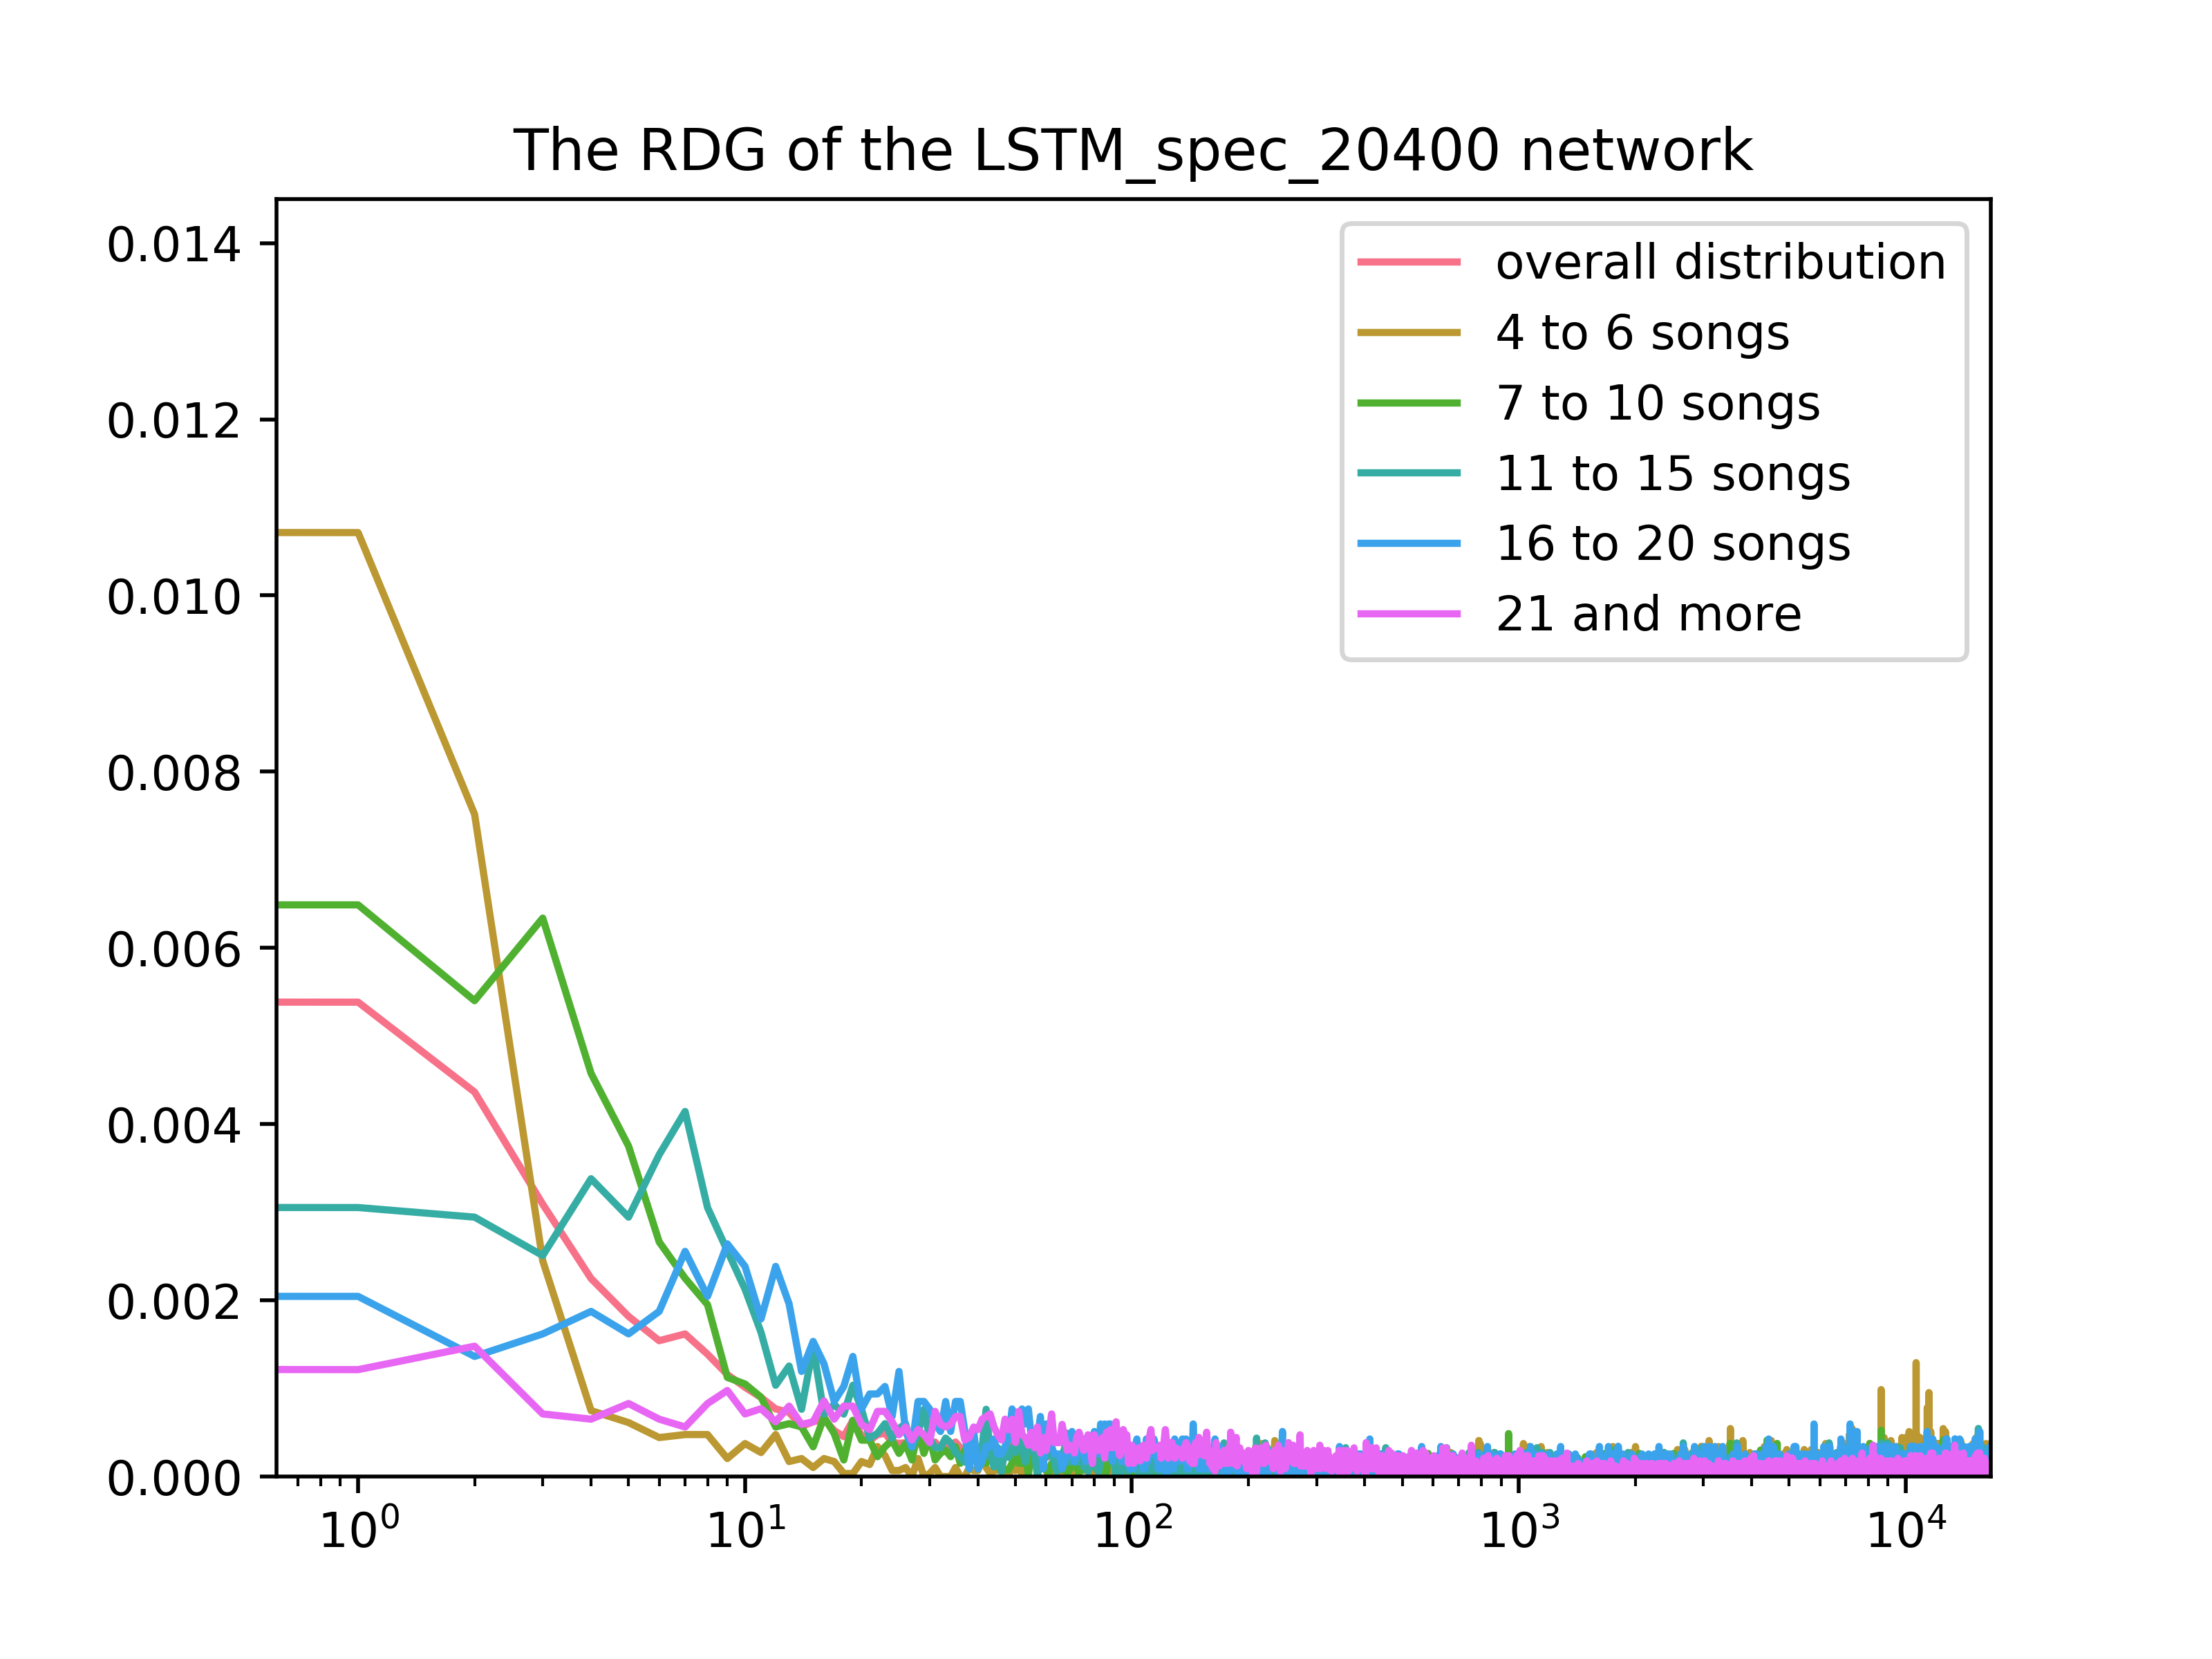
\includegraphics[width=1\linewidth]{./img/lstm_spec_20400_graph.png}
  \captionof{The distribution of predicted ranks using the long GRU spec encodings.}
  \label{fig:lstm_spec_20400_distribution}
\end{minipage}%
\begin{minipage}{.5\textwidth}
  \centering
  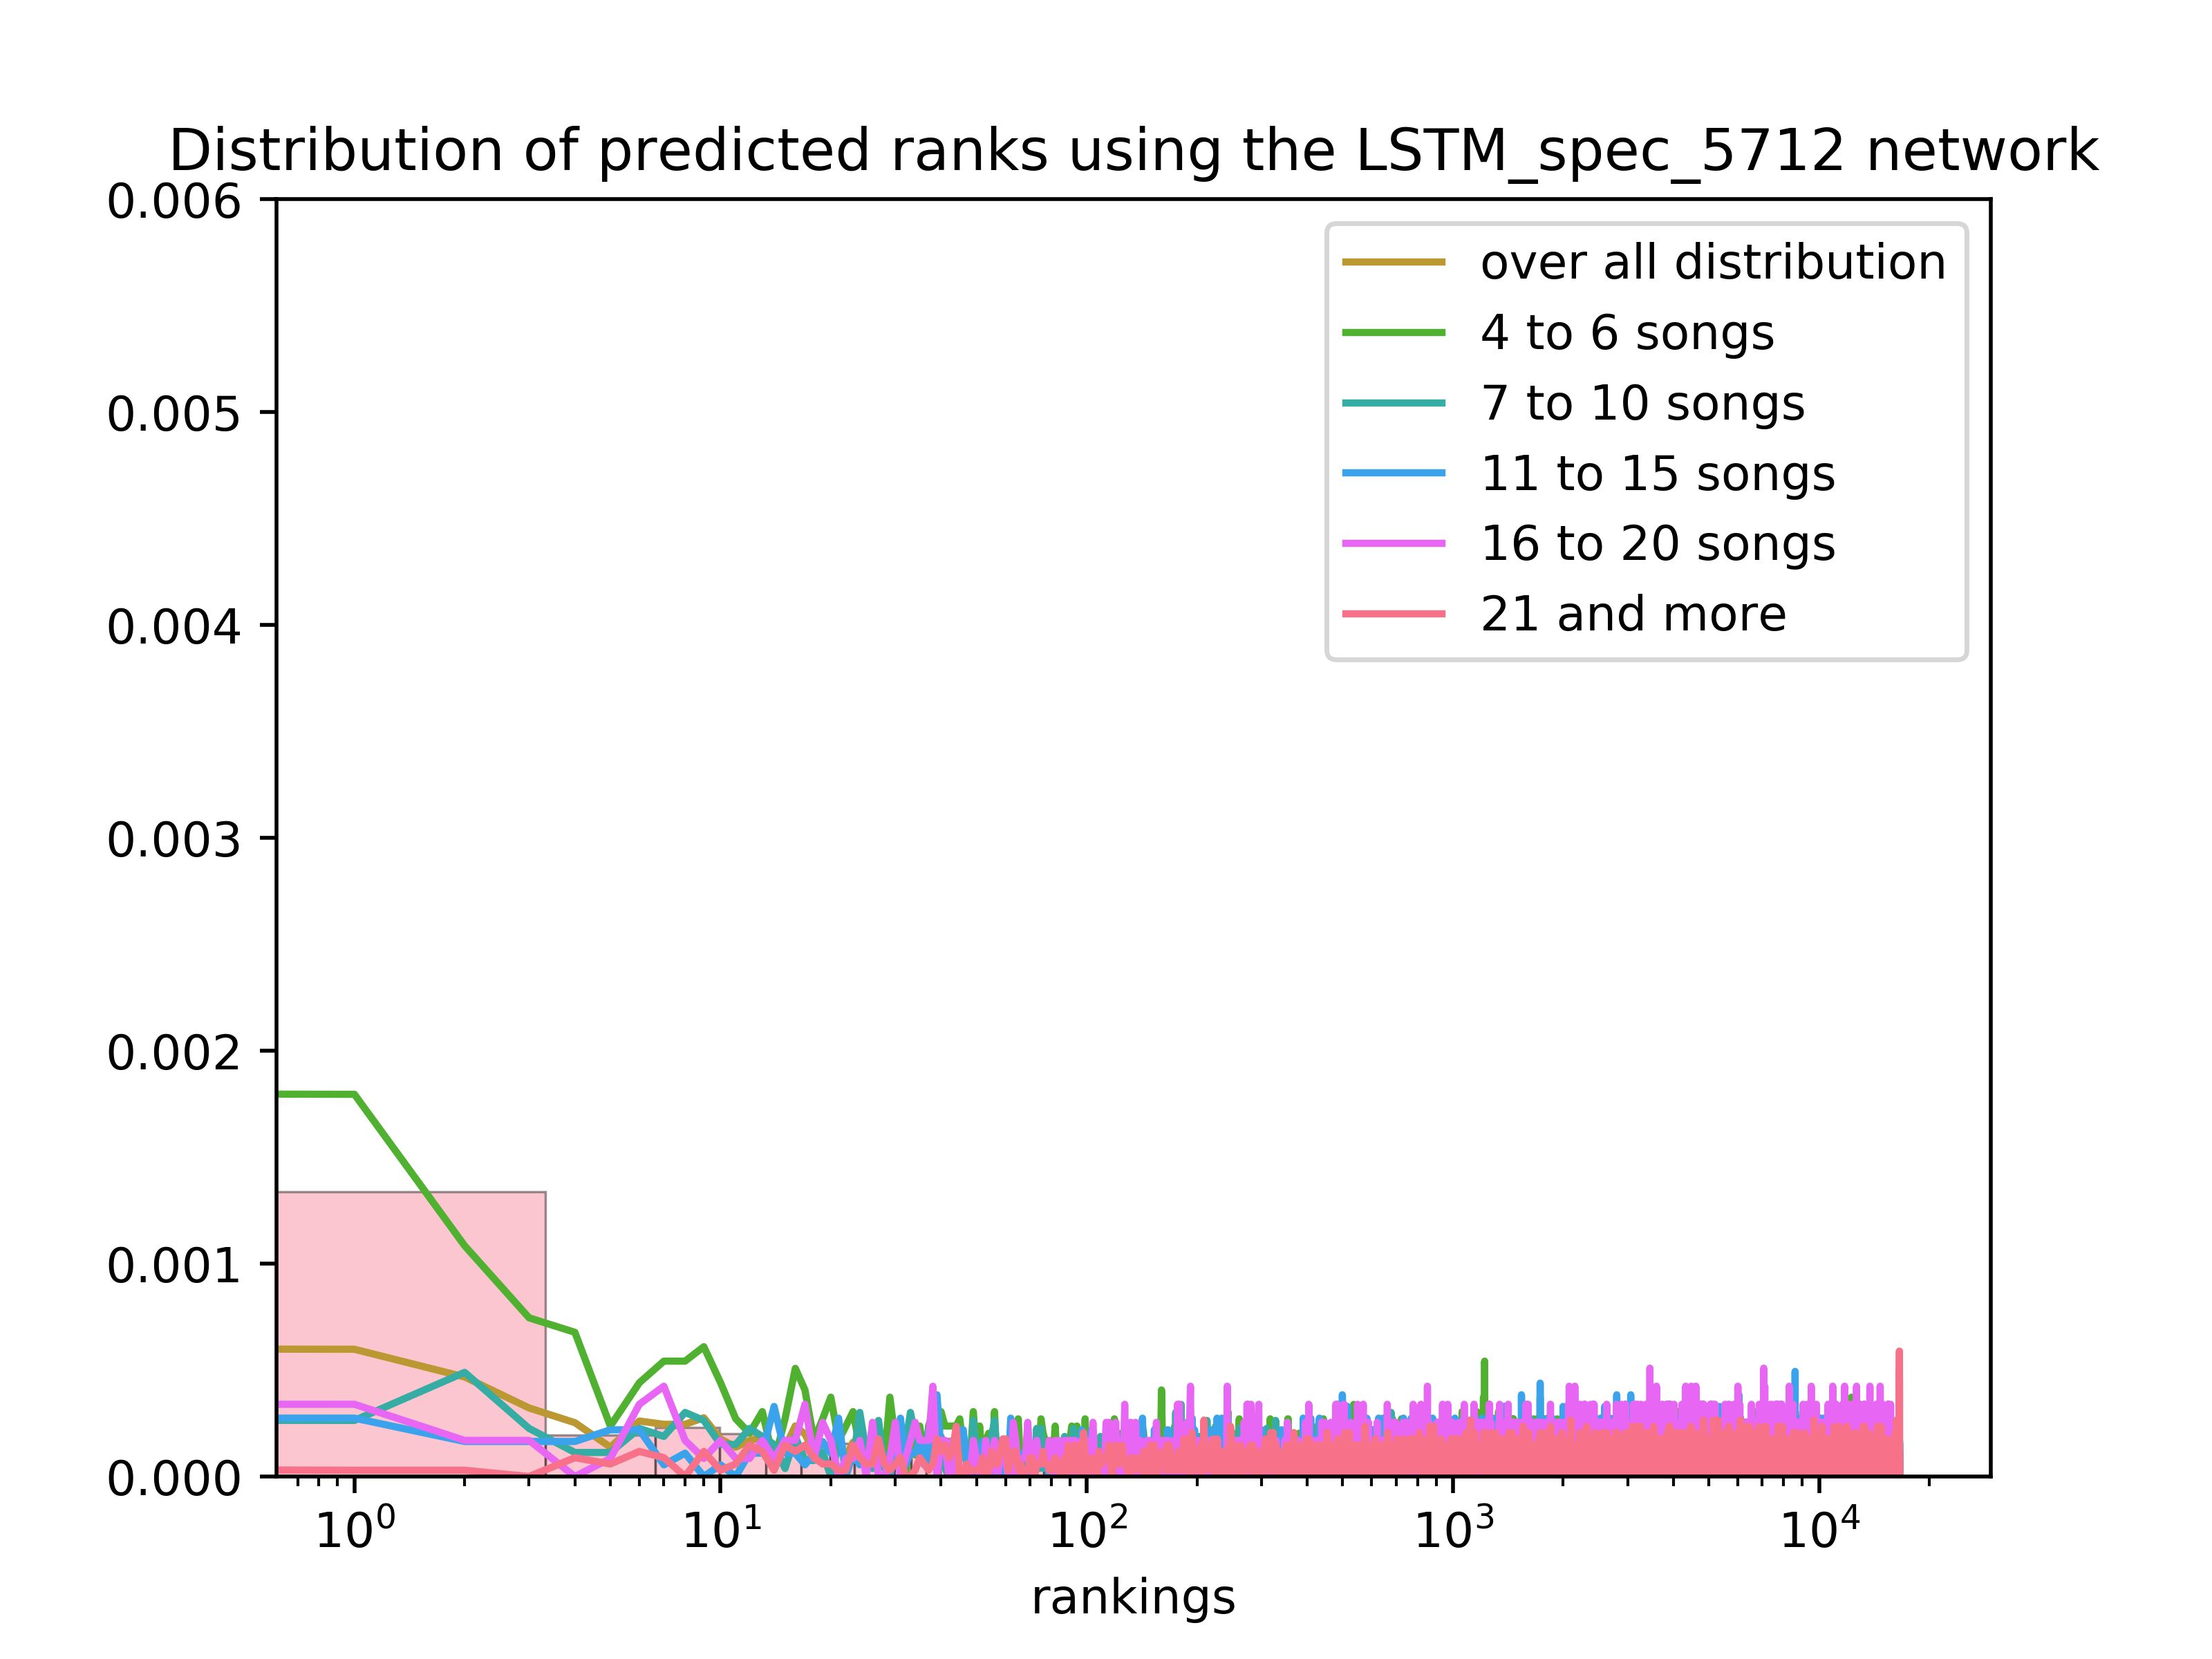
\includegraphics[width=1\linewidth]{./img/lstm_spec_5712_graph.png}
  \captionof{The distribution of predicted ranks using the short GRU spec encodings.}
  \label{fig:lstm_spec_5712_distribution}
\end{minipage}
\end{figure}\label{fig:lstm_spec_distributions}

\subsection{GRU and LSTM networks with Mel-spectrogram input}

\subsubsection{Training}
The GRU\_mel and LSTM\_mel networks were both trained under the same conditions. We trained them on our mel-spectrograms for 150 epochs with a batch size of 256. With a higher batch size we got a memory error. The output length of the encoded song vector was based on variance ratio of the PCA\_mel (same as for networks with neural networsk with spectrogram input). We did not attempt any further reductions here partly because further dimensionality reduction in PCA\_mel\_320 greatly hurt the performance and partly because as stated before, only the features can be reduced by GRU and LSTM layers meaning, that we have to have vectors of length of at least 408 and to scale the features down to one or two might lead to same results as with our SOM methods.

\subsubsection{Results}
Mel-spectrograms seem to be the best kind of input we have and the GRU\_mel and LSTM\_mel networks confirm it as they have the best results within the neural network method group. The GRU\_mel network performed better than the one with LSTM layers and also showed the smallest loss in training. The difference in ranking accuracy is quite big. Figure \ref{fig:mel_nn_distributions} exposes another thing worth noting which the big difference between short and long playlist rankings for both methods. \\
Table \ref{table:mel_spec_methods} puts recalls and nDGC of our "mel" neural networks into perspective with other "mel" methods.
As we can see, the GRU\_mel network placed 3.6\% of songs into the top 10, 4.3\% into the top 50 and 4.9\% into the top 100. This is worse than the raw mel-spectrogram method for \textit{R@10} but for \textit{R@50} and \textit{R@100} it shows better results. The GRU\_mel network is almost twice as bad and places as our second worst "mel" method with only 1.4\% of songs in the top 10, 2\% of songs in the top 100 and 2.6\% of songs with assigned ranks in the top 100.

\begin{figure}[h!]
\centering
\begin{minipage}{.5\textwidth}
  \centering
  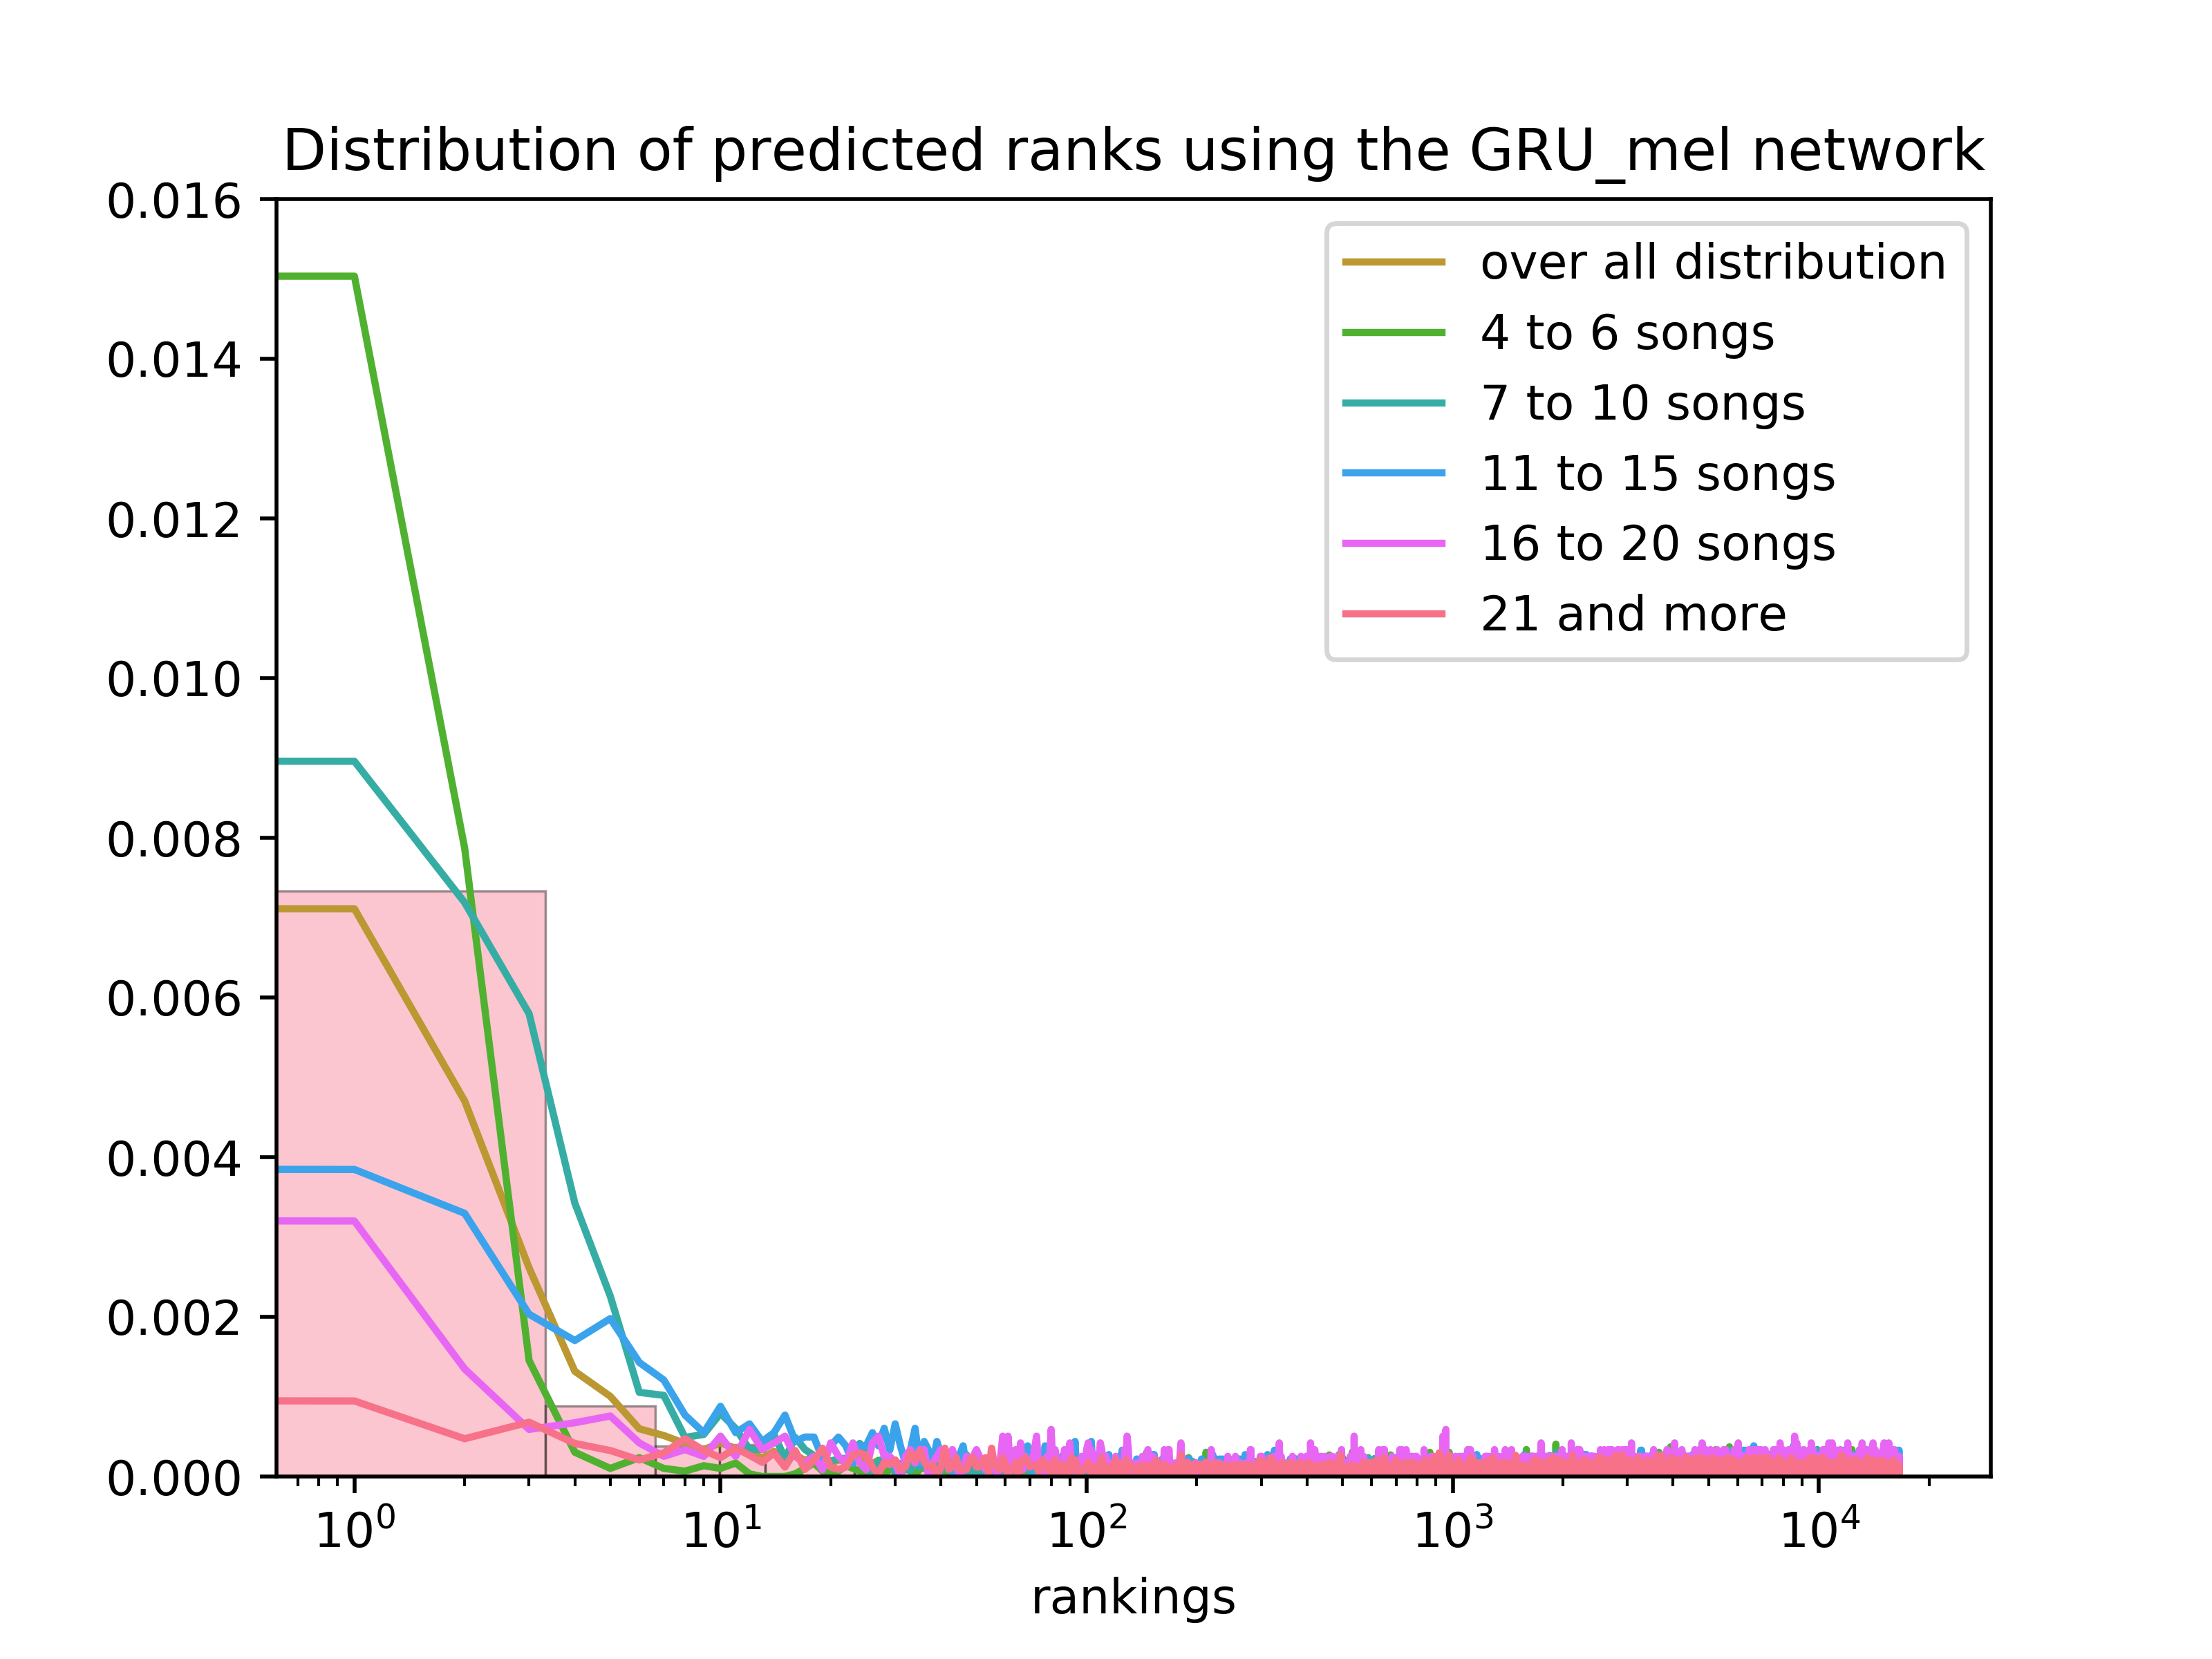
\includegraphics[width=1\linewidth]{./img/gru_mel_graph.png}
  \captionof{An RDG of the GRU\_mel method}
  \label{fig:gru_mel_distribution}
\end{minipage}%
\begin{minipage}{.5\textwidth}
  \centering
  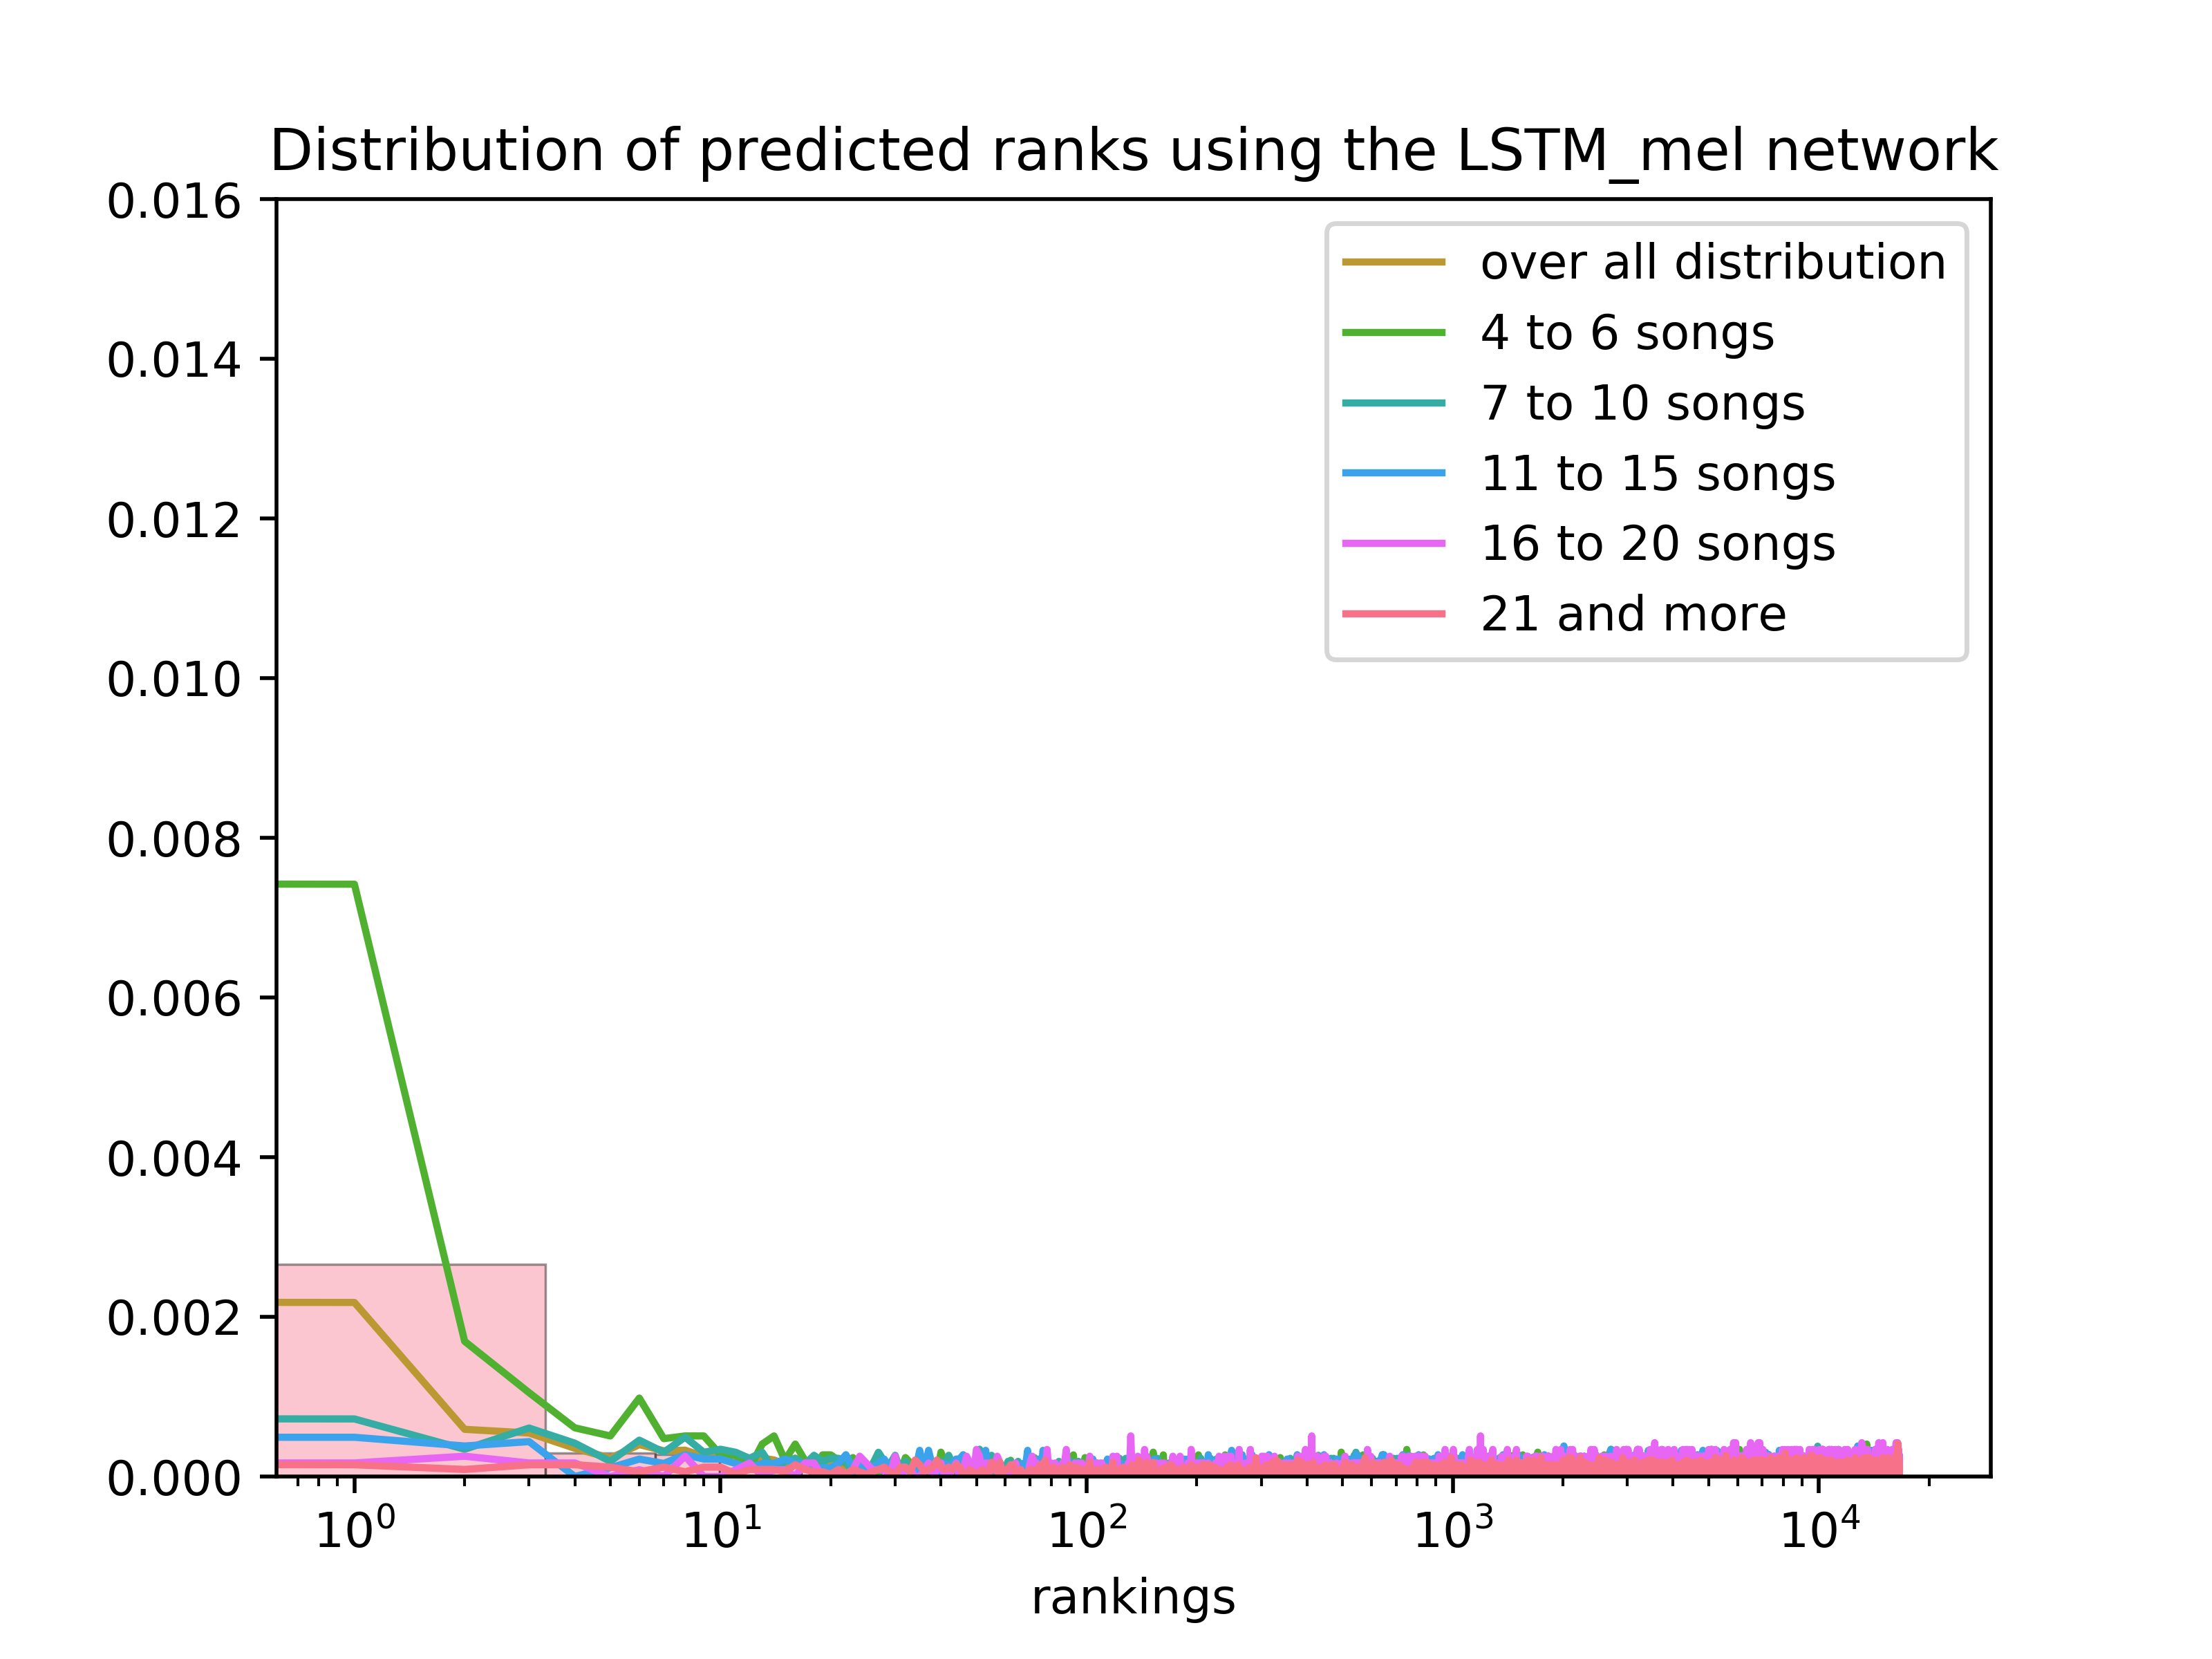
\includegraphics[width=1\linewidth]{./img/lstm_mel_graph.png}
  \captionof{An RDG of the LSTM\_mel method}
  \label{fig:gru_mel_distribution}
\end{minipage}
\end{figure}\label{fig:mel_nn_distributions}

\subsection{GRU and LSTM networks with MFCC input}

\subsubsection{Training}
At first we did not plan on using MFCCs as input into neural networks. However because it turned out the the raw MFCCs are too long to be used in our application directly we decided it would be a shame to just leave them out and tried to reduce their dimension again with both our GRU and LSTM network architectures. \\ 
We trained both architectures with 150 epochs and a batch size of 256 which is the same as the neural networks having mel-spectrograms as input. 

\subsubsection{Results}

The MFCC networks seem to have the biggest potential of improving if they were to be trained for a longer period of time as their plots in Figure \ref{fig:all_model_training} especially the GRU\_MFCC one does not stagnate as much as the other networks. They would however probably never decrease their loss to be as small as for the "mel" networks. \\
Compared to the raw MFCCs the GRU\_MFCC meant an improvement whereas the LSTM\_MFCC an impairment as the values in \ref{table:mfcc_methods} suggest. The Figure \ref{fig:mfcc_nn_distributions} containing both method's \textit{RDGs} confirms the superiority of the GRU\_MFCC method over the LSTM\_MFCC. What is interesting about the LSTM\_MFCC is the fact, that the ranks for shorter playlists are not as notable as with most other methods like for example the GRU\_MFCC method where the difference is considerable.

\begin{figure}[h!]
\centering
\begin{minipage}{.5\textwidth}
  \centering
  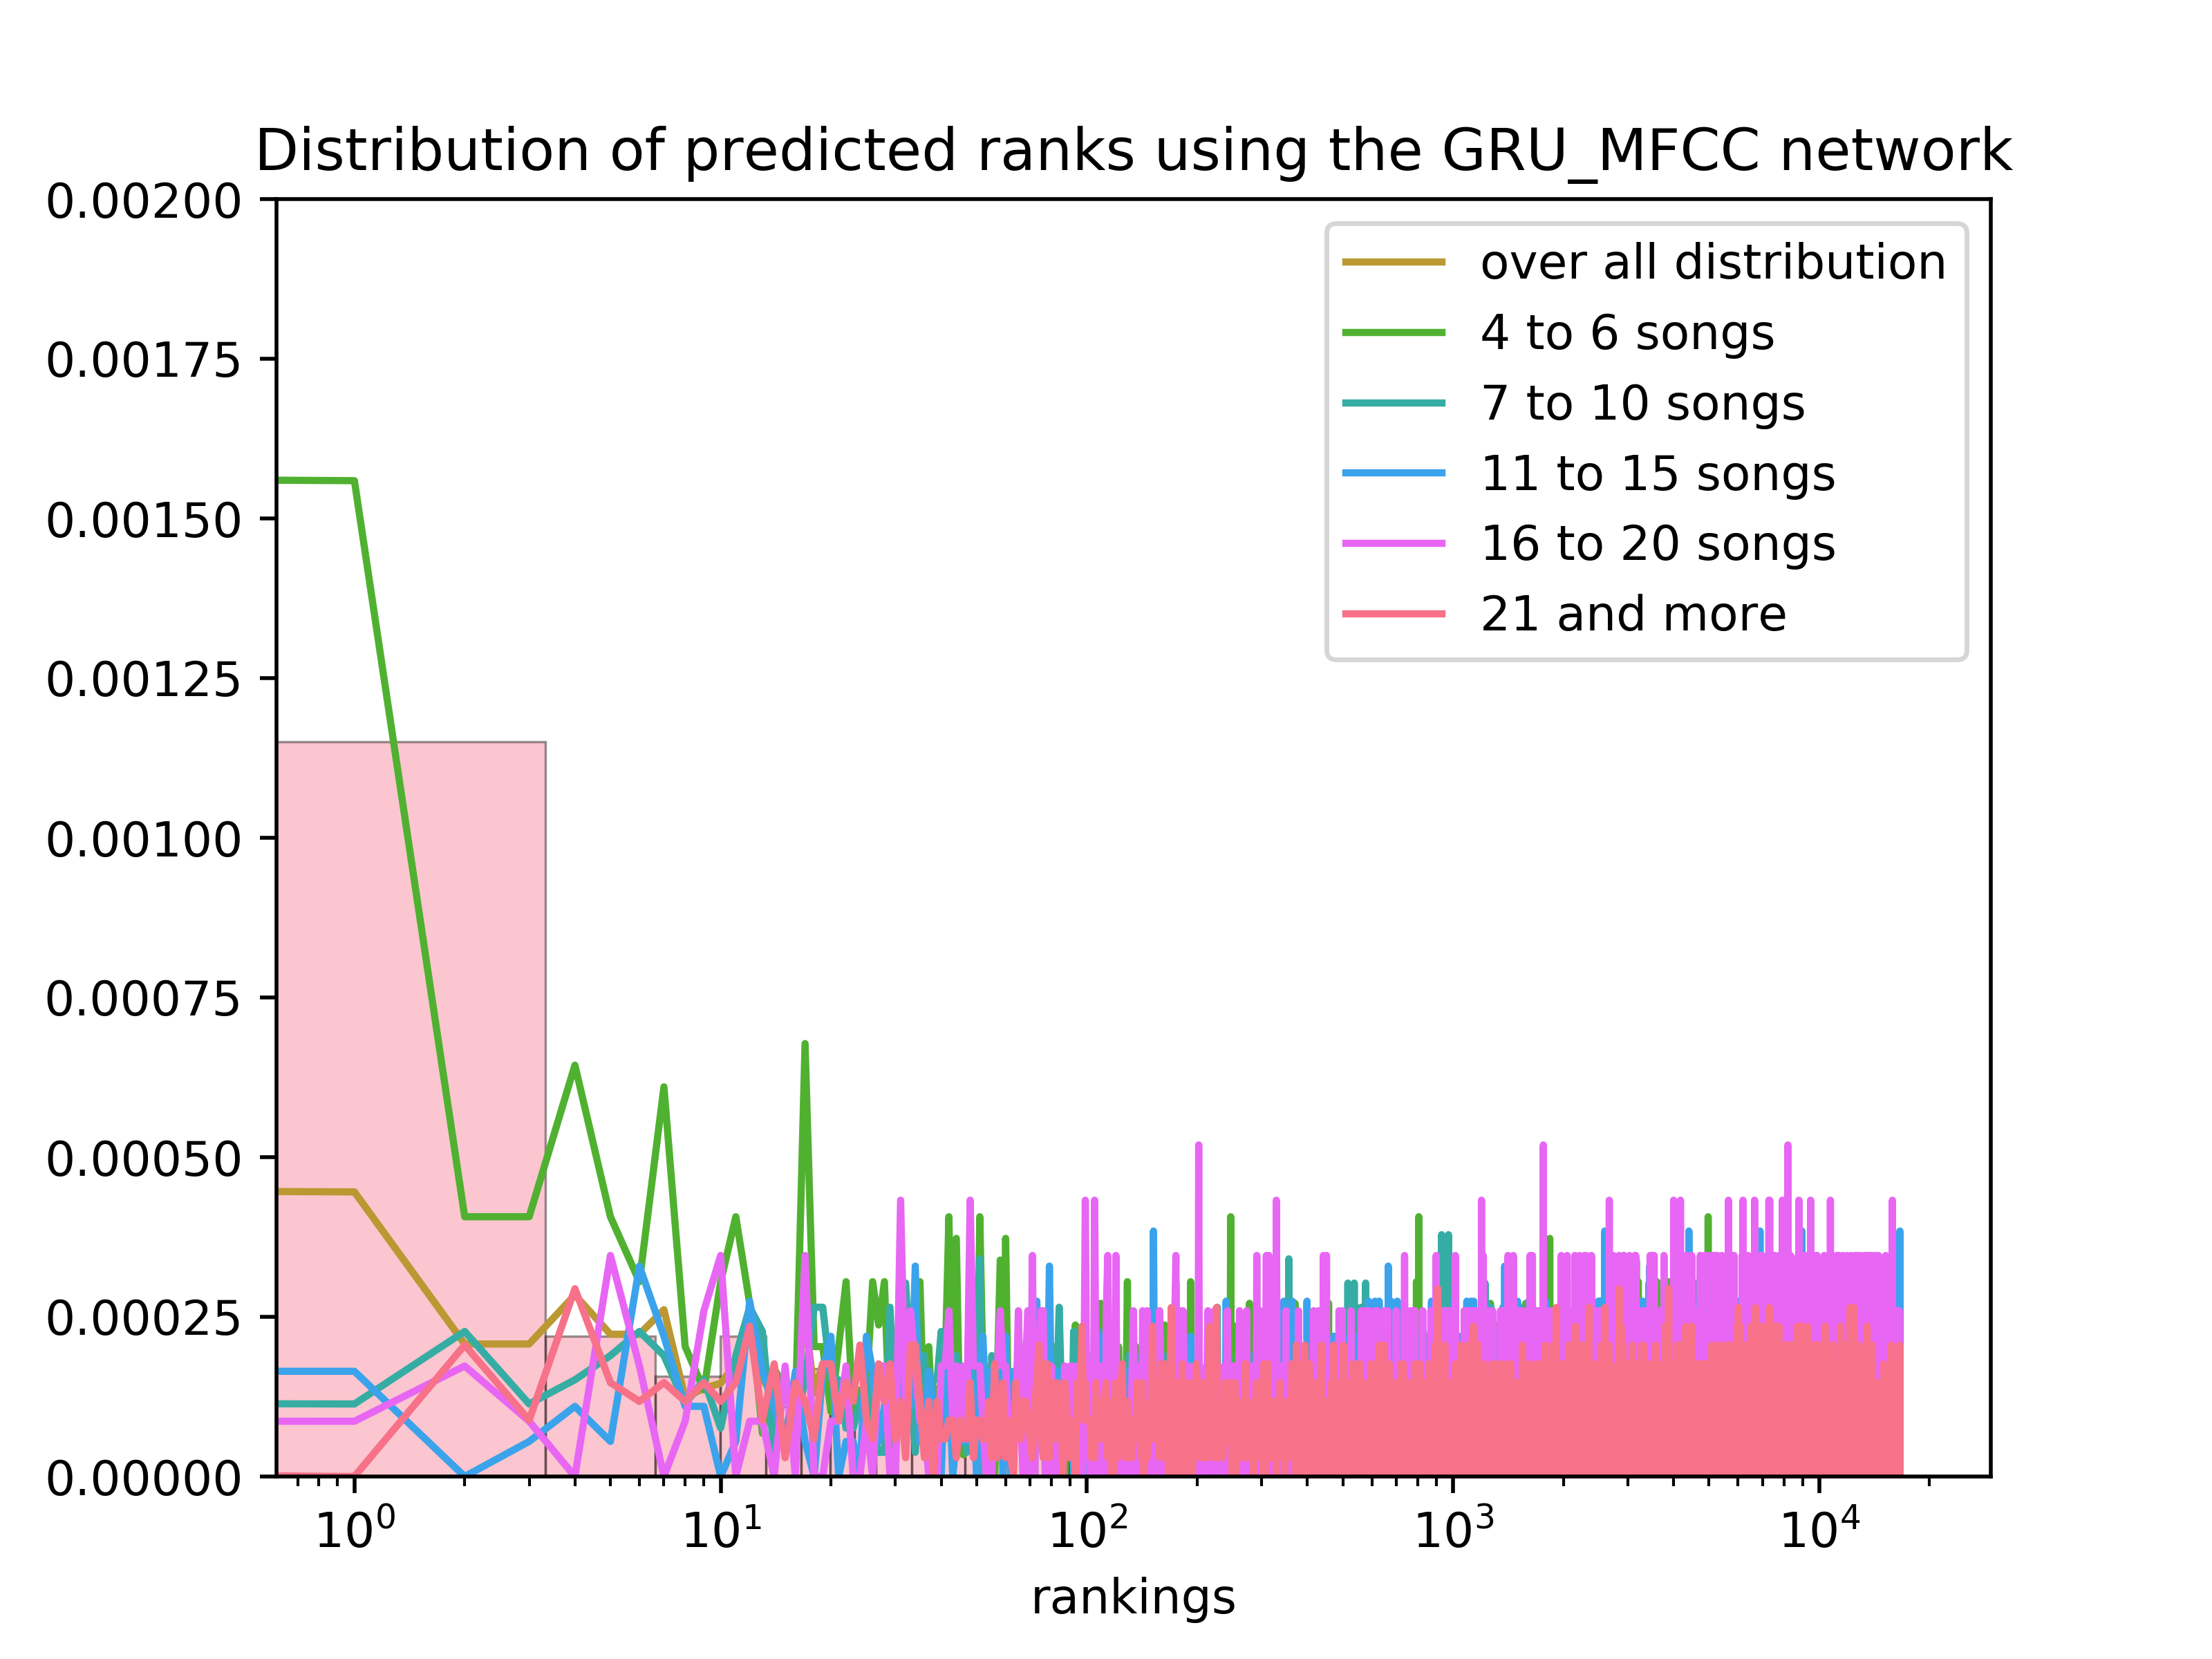
\includegraphics[width=1\linewidth]{./img/gru_mfcc_graph.png}
  \caption{The RDG of GRU\_MFCC}
  \label{fig:gru_mfcc_distribution}
\end{minipage}%
\begin{minipage}{.5\textwidth}
  \centering
  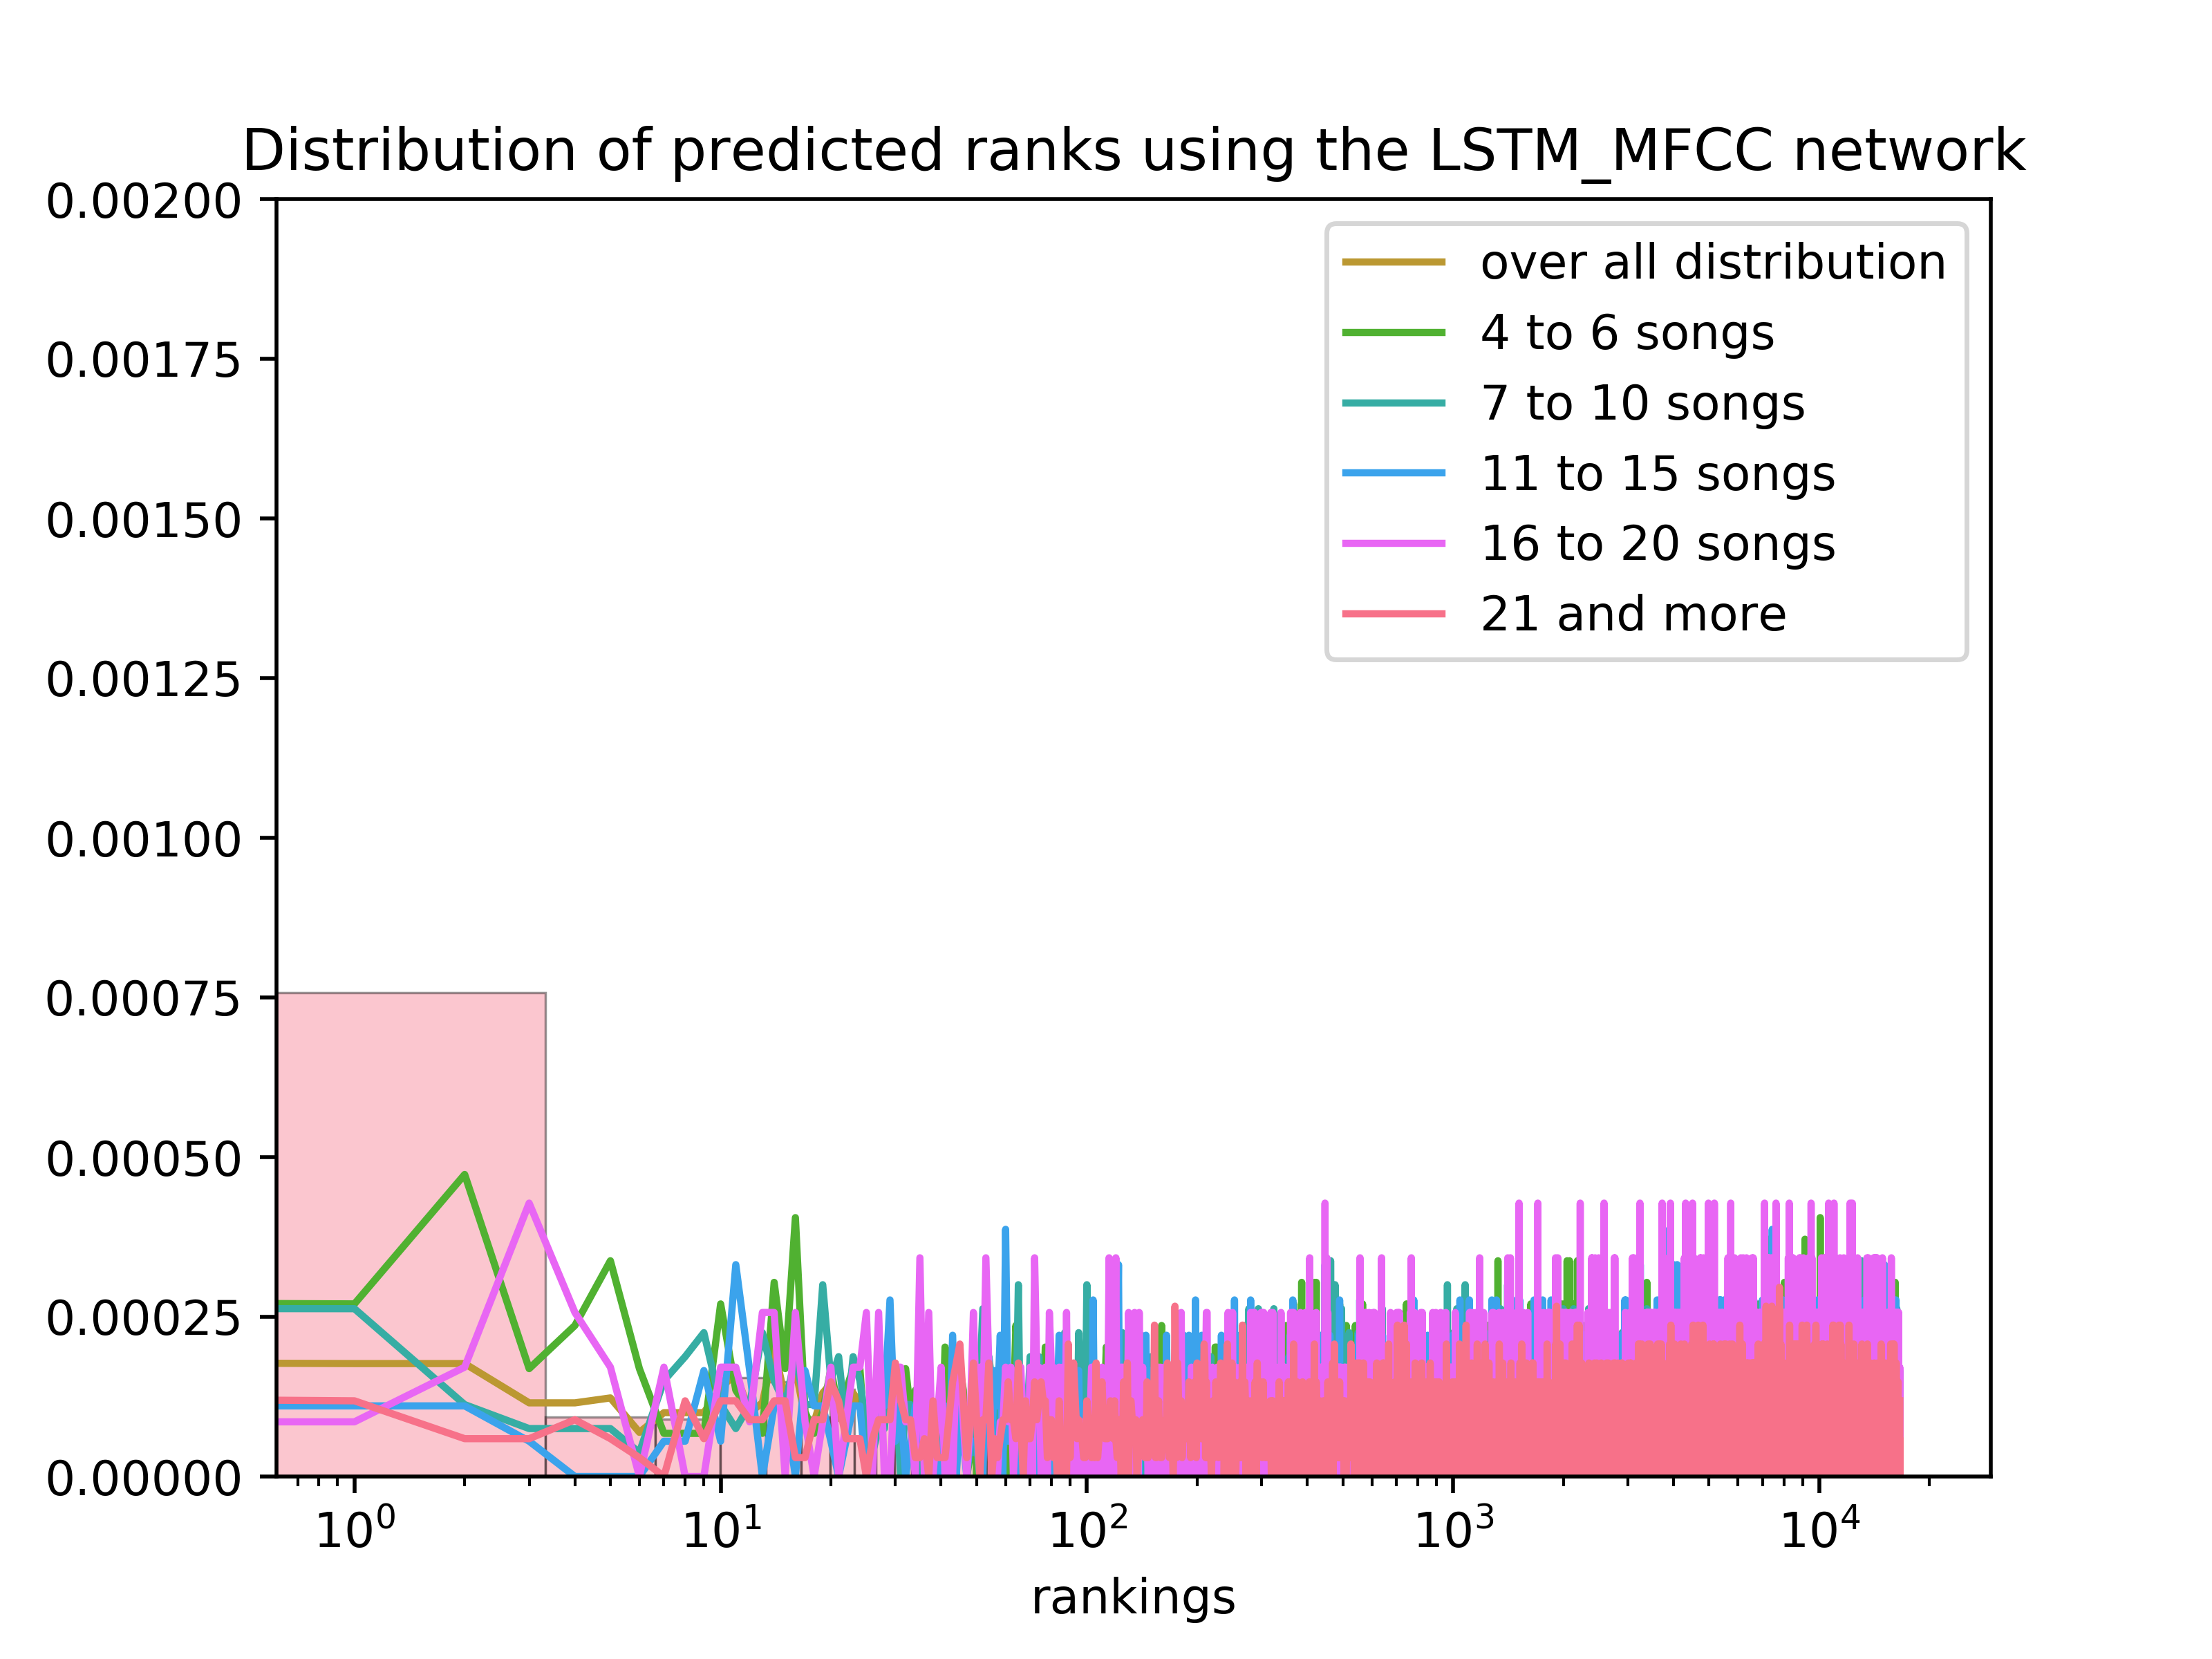
\includegraphics[width=1\linewidth]{./img/lstm_mfcc_graph.png}
  \caption{The RDG of LSMT\_MFCC}
  \label{fig:gru_mfcc_distribution}
\end{minipage}
\end{figure}\label{fig:mfcc_nn_distributions}



\section{Discussion}\label{sec:discussion}

All the experiments we performed yielded a lot of data, to be fair more than we planned. In this discussion we try to compare our findings with the expectations we had and interpret their similarities and differences. Overall we have to admit that the results we obtained were worse than we thought they were going to be. We will try to explain the reasons. \\
The thing that was apparent in almost all methods was the decrease of top ranking for songs from $ p_{test}$ that were a part of a longer playlist. We thought that this is actually a thing that we could fix. The fact that shorter playlists have better rankings suggests that the users have groups of songs in their playlists that are very similar to each other but the groups can be quite dissimilar and that songs, that are somewhat similar to all groups "pollute" the recommendations. Therefore, we decided to evaluate all methods again with a distance threshold. We actually meant to do this even before we knew that our methods perform better on shorter playlists because we thought that it is better not to save all distances into the web-applications database but only the top $n$. \\
We chose the threshold separately for each method as the 846297th biggest similarity. It may seem as a strange random number but is is $51*|dataset|$ where . It gives us about 50 most similar songs for each song and the additional 1 is to get 50 even though we will always include the most similar one which is the same one. \\
This significantly changed and in many cases improved the performances of our methods. We decided not to include all the new distribution graphs again, \todo{Mohla bych je dat do attachmentu} but we decided to include at least a table comparing the other evaluation measures we chose. \todo{SEM dat table nebo graf? tech novejch metod}.\\

Even with the threshold improvement, our results are still worse than we were hoping for. 
\begin{figure}[h]
    \centering
	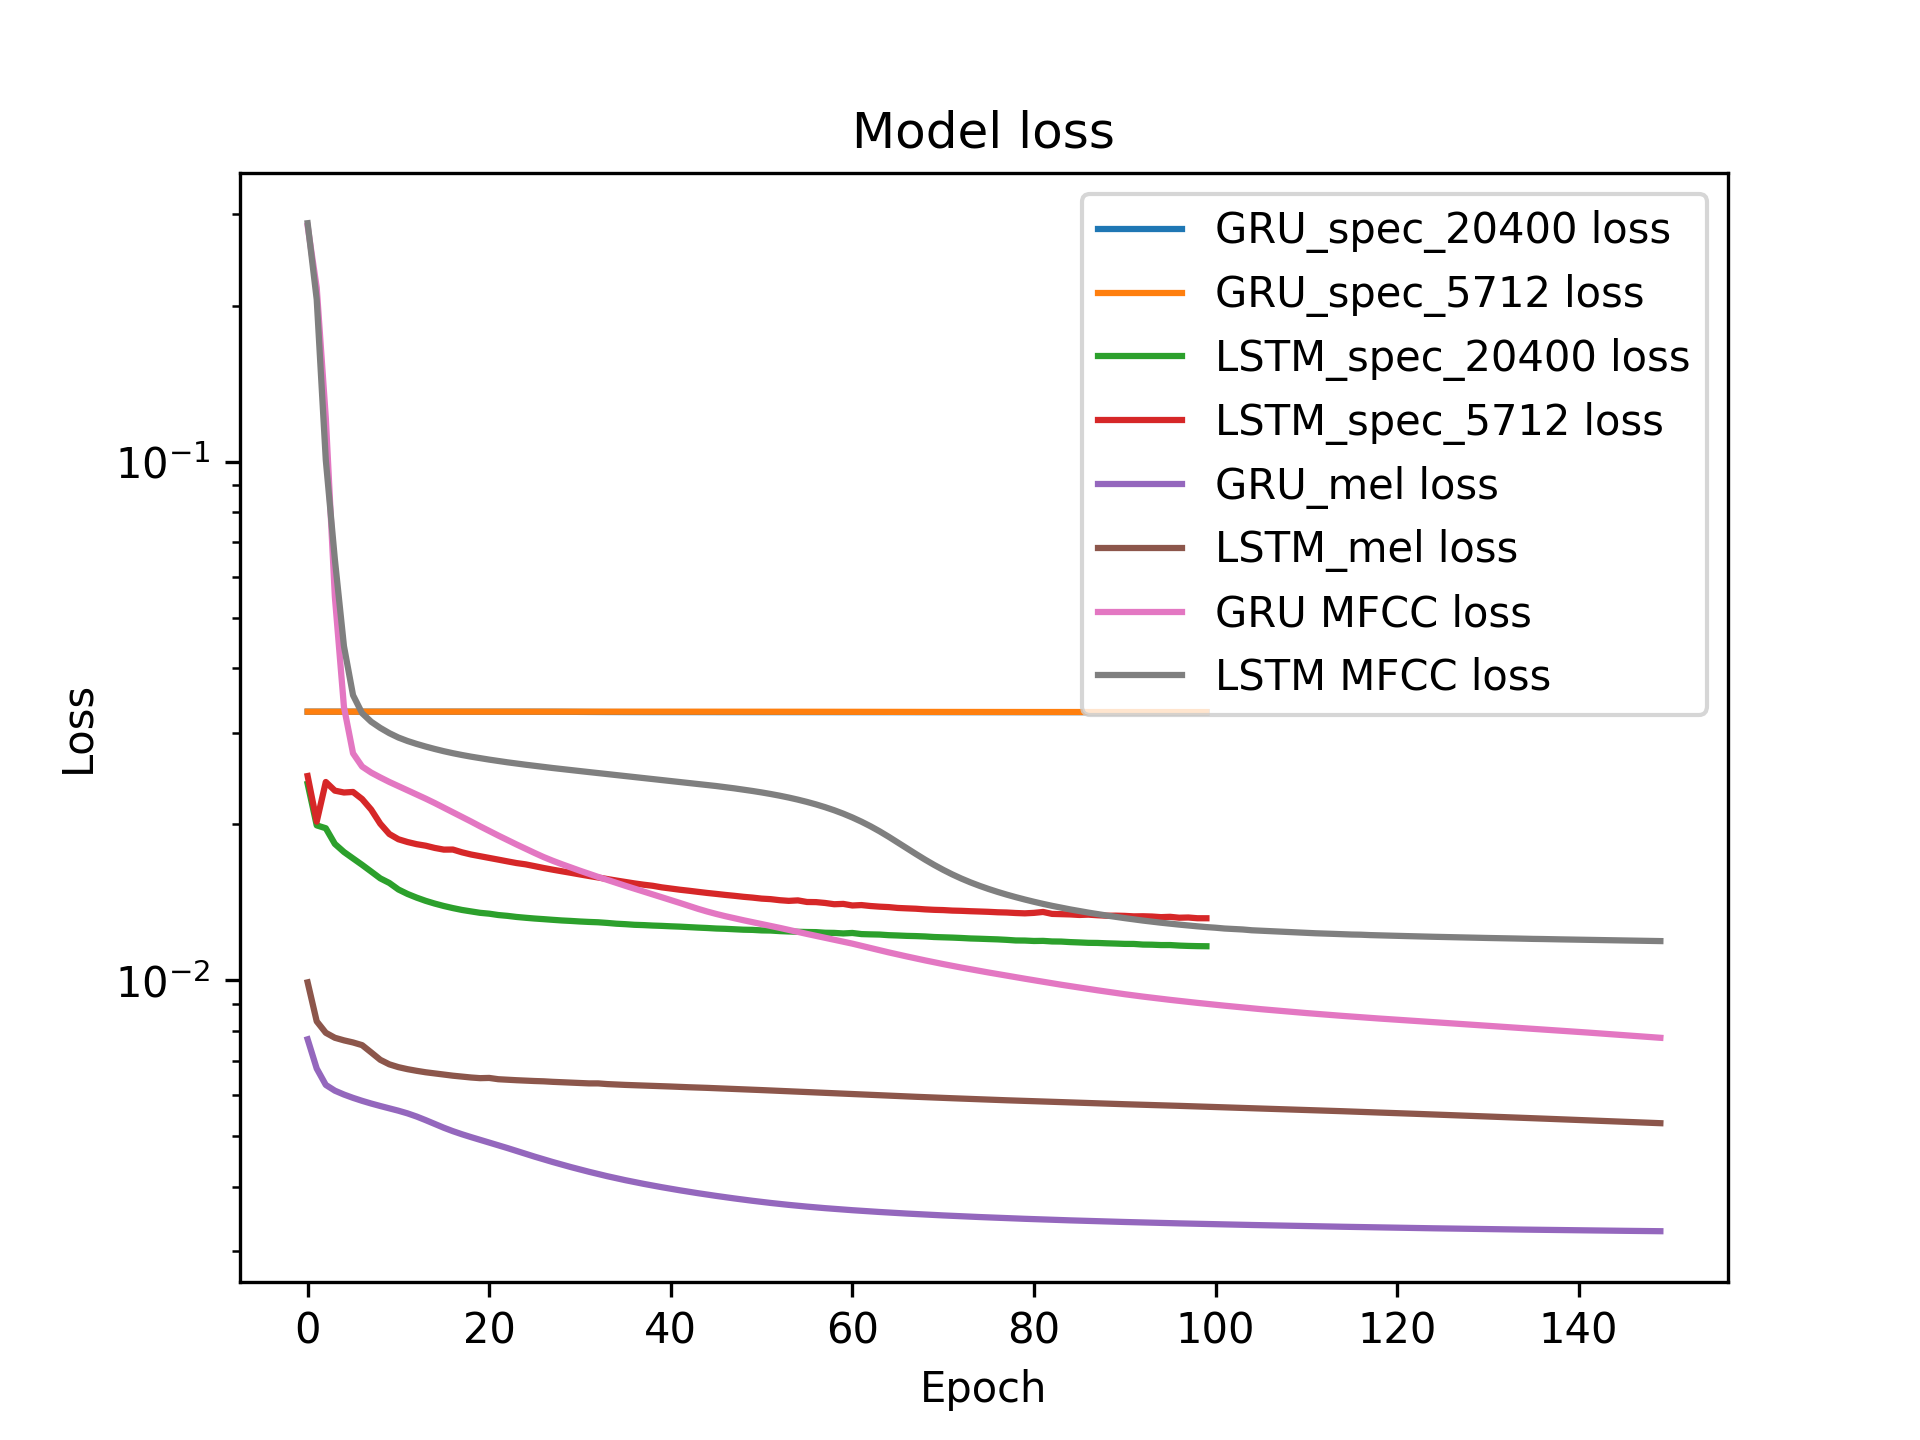
\includegraphics[width=120mm]{./img/all_training_graphs.png}
	\caption{The training mean squared error loss values for all the final neural networks we trained.}
	\label{fig:all_model_training}
\end{figure}
%\chapter{Web Application}
\todo[inline]{LP: zkuste to po sobe jeste precist. Pozor treba na jednotne/mnozne cislo (application vs. applications). Mit vetu pres 4 radky taky neni zrovna nejlepsi. Klidne se to da vic rozepsat. In this section, we will describe the proposed web application for novel song recommendation. The section is structured as follows:...

Celkove bude potreba, abyste se na to jeste podivala a zapracovala na preciznosti formulaci - muj pocit z te kapitoly je cca "no jako rozumim tomu, ale proc to proboha napsala takhle divne". Par prikladu jsem vyznacil nize v textu, ale je jich vic. Spis by stalo za to to poradne projit a prepsat - a ja na to mrknu detailneji az tohle probehne...}
In this section I will describe the features of the applications and the user interface in the \textbf{Analysis} section, the design chosen for this application with some high-level developer documentation in the \textbf{Design} section, possible developer configurations in the \textbf{Configuration possibilities} section and some high-level user documentation in the \textbf{User Documentation} section.

\section{Analysis}
\todo[inline]{LP: Takhle bohužel ne. Vy tady popisujete seznam naimplementovanych vlastnosti, tak by ale analyza fungovat nemela. Vy tu primarne chcete popsat, co uzivatel od vasi aplikace muze ocekavat - tasks a jakym zpusobem je chcete uchopit. Takze to co tu pisete je spise zaver analyzy, ale chybi k tomu nejaky uvod... Muzete take provest srovnani s jinymi systemy typu youtube/spotify a zakladni pozadavky uzivatelu od toho odvodit, pak pridat to cim se vymyka vas system - jde primarne o nalezeni noveho a jen o hudbu a na zaklade toho sestavit navrh implementovanych funkcionalit, pripadne i definovat dalsi pozadavky na system...}
The is in English \todo{LP: wtf?}. It requires users to create a unique username and password (there will also be a possibility of e-mail authentication - see section 6.3). For a logged in user, there are multiple functionalities. \\
From any page there are multiple redirection possibilities through a navigation bar. 
\begin{itemize}
    \item The \textit{Homepage} displays a truncated list of songs recommended to the current user. The user will also see a list of \textit{playlists} he created.
    \item The \textit{Recommended} page displays just a longer list of songs recommended to the user and also songs he played.
    \item The \textit{My lists} page displays all of the current users playlists along with first 10 songs and a list of songs recommended based on those in the particular list. From here, the user can create a new list or go to any \textit{List detail} page.
    \item The \textit{Add song} page is a form to add a new song. The lyrics and YouTube link are mandatory as well as the song and artist name. Songs added by any authenticated user are visible and recommendable to all the users. It is not possible to add a song that is already in the database.
    \item The \textit{All songs} page displays all songs that are in the database in ???alphabetical??? order.
    \item The \textit{Distance type} drop-down does not redirect the user to a different page but only changes the criteria for calculating and displaying recommended songs. The choices are based on the findings of this work: \begin{itemize}
        \item TF-idf
        \item Word2Vec
        \item \textit{??? Textova metoda ???}
        \item \textit{??? PCA}
        \item \textit{??? Neural network embedding}
    \end{itemize}
    \item The \textit{Search} input area and button search artists, songs titles and combination of those two based on what the user fills into the input area. The 10 best matches are displayed.
    \item The \textit{Username} drop-down lets the user log out.
\end{itemize}
There are also other redirection possibilities the user can access from only specific pages, not the navigation bar common for all the pages.
\begin{itemize}
    \item The \textit{Song detail} page displays an audio file where it is possible to play the song, songs most similar to this song (based on the users current distance-type selection), a possibility to \textit{like} or \textit{dislike} the song and also a \textit{add to a list} option.
    \item The \textit{List detail} page displays has the same structure as the \textit{Homepage}\todo{LP:. However,...} but instead of recommendations based on all songs, the recommendation is based only on songs from the particular list and also songs from the particular list are displayed.
    \item There are also possibilities to \textit{Add} and \textit{Delete} lists the user has created. No option like this for played songs though\todo[inline]{LP:Nonetheless, there are no options... (sentence fragment)}. Disliked songs do not appear in the played list listing. 
\end{itemize}
A simplified visualization of the request handling flow of the application is shown in Figure 6.1.

\begin{figure}[h]
    \centering
	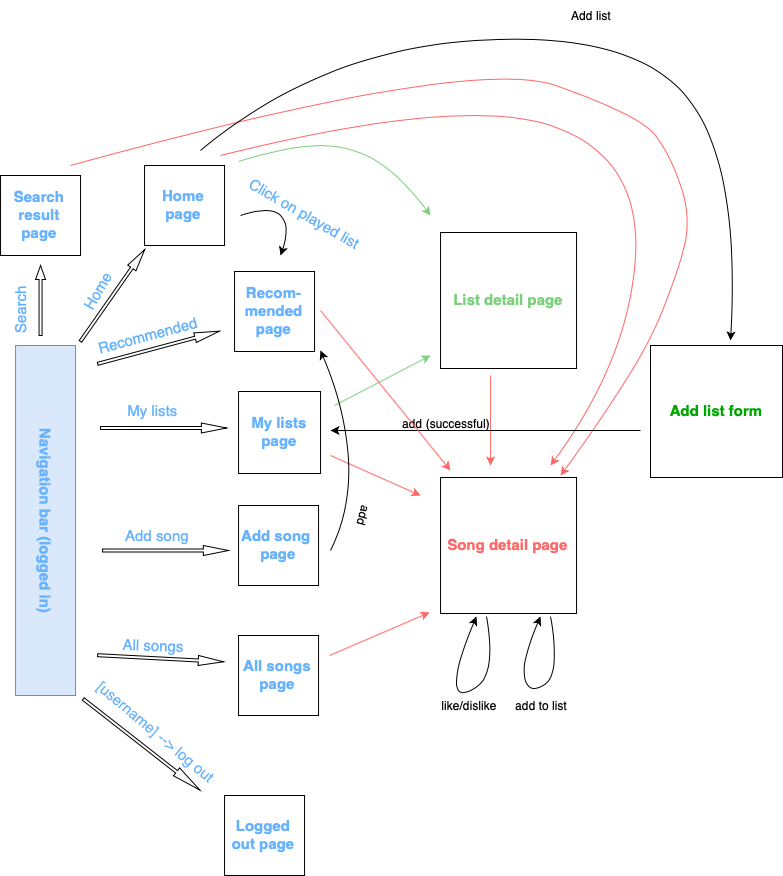
\includegraphics[height=120mm]{./img/analysis_diagram.png}
	\caption{Request diagram}
	\label{fig:analysis}
\end{figure}

\section{Design}
\todo[inline]{LP:Jak se na to divam, tak bych zmenil nazvy - tohle je spis Implementace a predchozi sekce - potom co ji dodelate by mohla byt analyza a design}
 To create the web application I used a web framework Django based on Python 3.7. The database used is PostgreSQL and to detach long computations that occur from user requests, I used the Celery asynchronous task queue with RabbitMQ as a broker.\\
 \todo[inline]{LP: Sem by se hodilo lehce popsat co jsou ty zminene technologie a proc jste si vybrala zrovna ty a ne neco jineho - jake jsou treba vyhody pythonu proti jinym variantam, proc zrovna celer s kralikem, co prinasi Django}
 The application consists of two main parts. The application itself (the client, server, models and views) and the similarity computation algorithms.
 
 \subsection{Application}
 
 \subsubsection{Client}
 
 The client has access to multiple html pages, all except of sign-up upon login. All the pages are Django templates written using HTML5 and some CSS for nicer design. \\
 
 The html pages \texttt{add\_song\_failed.html} \texttt{add\_to\_list\_failed.html}, \texttt{addSong.html}, \texttt{all\_songs.html} \texttt{index.html}, \texttt{list\_confirm\_delete.html} \texttt{list\_detail.html}, \texttt{list\_form.html}, \texttt{my\_lists.html}, \texttt{recommended\_songs.html}, \texttt{search\_results.html}, \texttt{song\_detail.html} these handle most of the interaction with the user and in-application functionalities. \\
 There are also special pages handling the user login and account \texttt{logged\_out.html, login.html, password\_reset\_complete.html, password\_reset\_confirm.html, password\_reset\_done.html, password\_reset\_email.html, password\_reset\_form.html, account\_activation\_email.html, account\_activation\_sent.html, signup.html}. \\
The page \texttt{base\_generic.html} is a base for all the html pages to keep the design consistent.

\subsubsection{Server}

The server does all the calculations in this application. To ensure a smooth user experience, the calculations are being sent to a task queue handled by Celery. This is possible because the computationally expensive requests users make do not need to be executed in a prescribed order. Those include:
\begin{itemize}
    \item adding a song, where the songs distance to all the songs in the database has to be computed for all the implemented distance-types of the application.
    \item liking and disliking songs as then the distance for all songs to the user and possibly to all lists the user has created needs to be recalculated
    \item adding a song to a list as all the other song distances to this list need to be recalculated
\end{itemize} 

\subsubsection{Database}

 The database is structured as the the Figure 6.2 displays.\todo[inline]{LP:The data structure is depicted on the Figure \ref{label obrazku} - takhle byste se z toho zblaznila, psat to vsechno rucne:-)} The user-related tables Django \todo{LP:tahle veta je trochu divna} automatically generates are omitted. The key tables are the \textit{Song}, \textit{Distance}, \textit{Profile} and \textit{List} table that store the main object the application uses. The others are there mostly to make make the system more clear and give easier access to desired objects. More specific description is provided in the \textbf{Model} section (6.2.?)
\begin{figure}[ht]
    \centering
	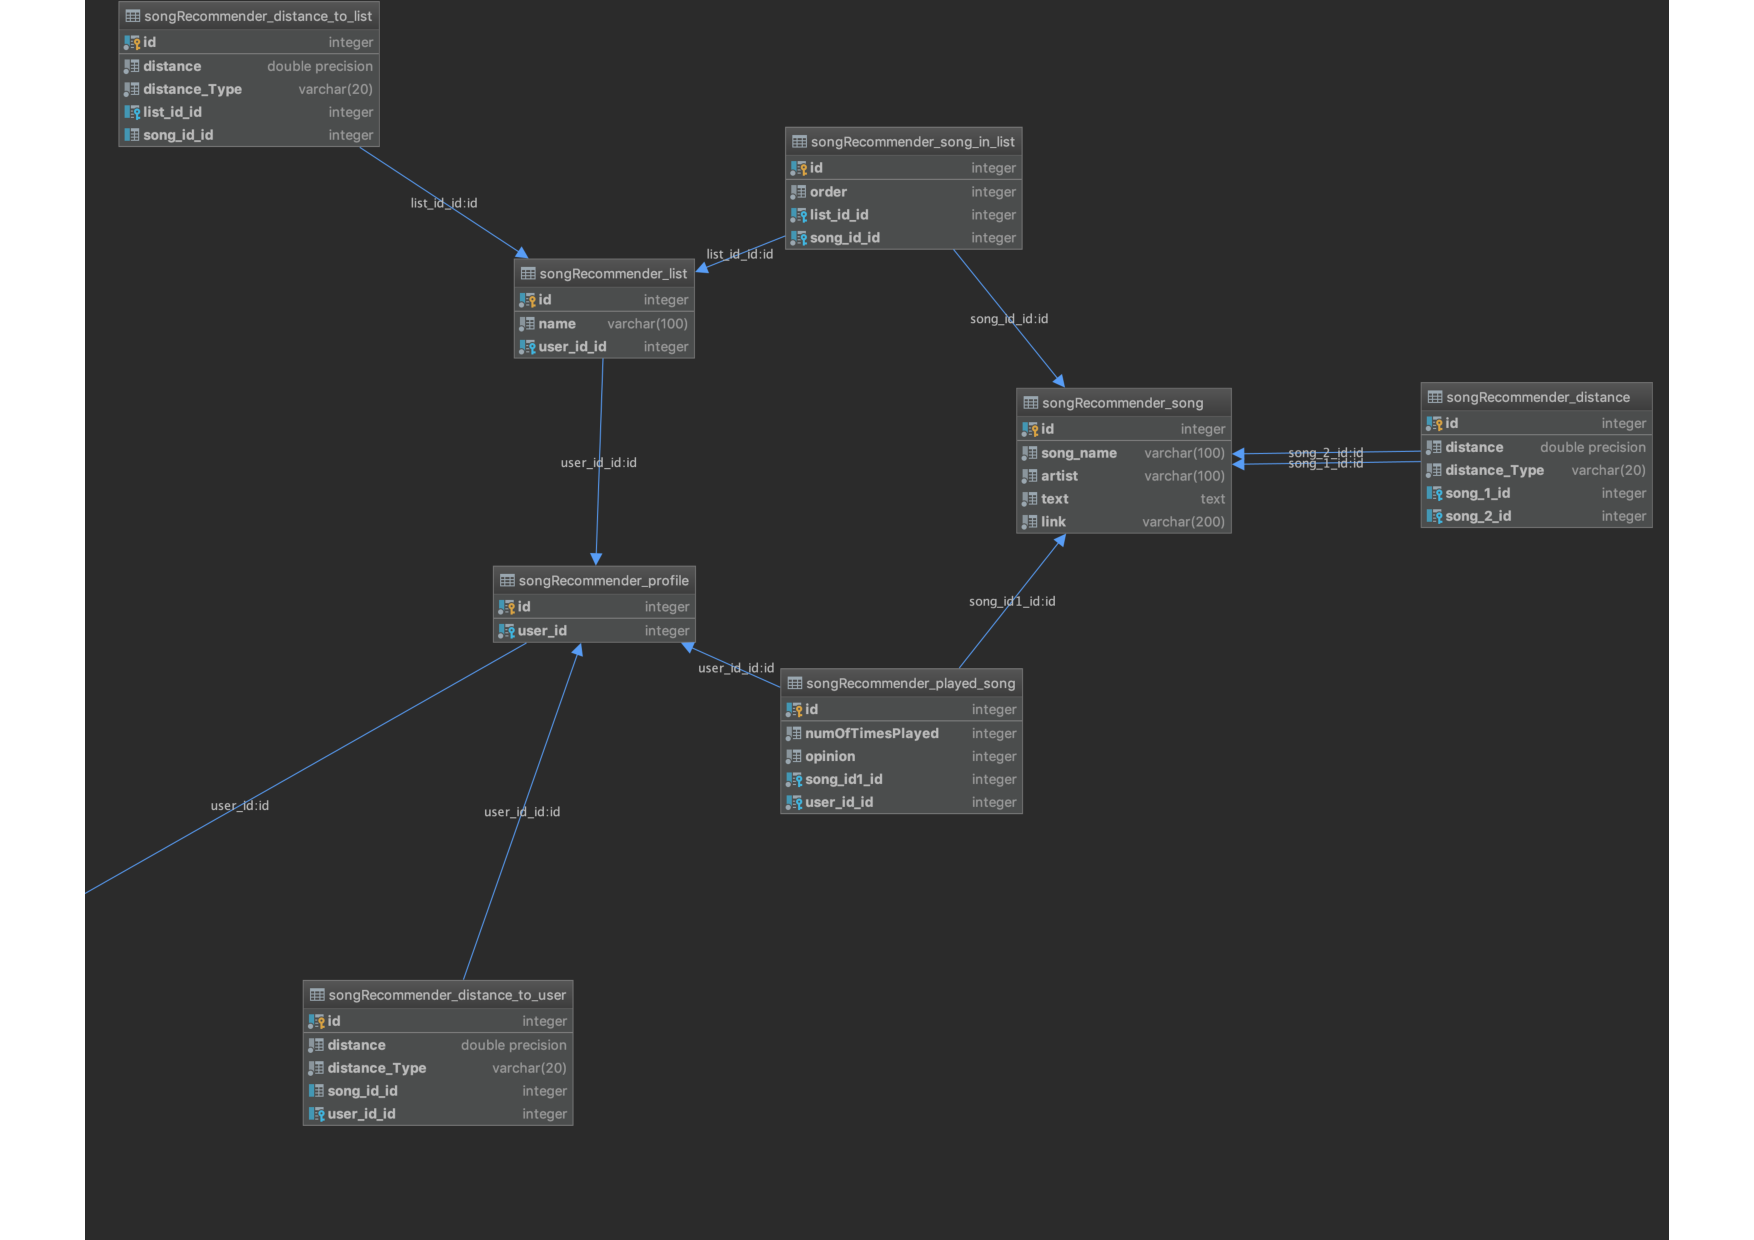
\includegraphics[width=120mm]{./img/database_diagram.pdf}
	\caption{Diagram of the applications database}
	\label{fig:diagram}
\end{figure}
 
 \subsubsection{Models}
 
 For every table in the database, there is a class-based model in the module \texttt{models.py} specifying their features. There is a class of the same name for \texttt{Song} and \texttt{List} table. The \texttt{Profile} model which is an extension of the build-in \texttt{User} model is included to enable specifying the distance of songs to the user and also checking if the user has confirmed his email.\\
 
The class \texttt{Song\_in\_list} keeps track of lists and songs that belong together, the model \texttt{Played\_song} specifies a user and all the songs he has played. One cannot un-play a song but it can be disliked and it will not appear anymore. \\

There are three different distance classes corresponding not to the way there were computed but corresponding to what distance they measure.\todo{LP: zase jedna divna veta.} First, the basic \texttt{Distance} class is the only class that actually stores distance based on a calculation of a similarity measurement algorithm. The classes \texttt{Distance\_to\_user} and \texttt{Distance\_to\_list} then calculate their distance data based on what they find in the \texttt{Distance} table using an algorithm from the module \texttt{tasks.py}.
 
\subsubsection{Views}

Views manage most of the data collection and send them as context to the html pages. There is one view for basically every html page plus some additional ones for some build in features for example liking and disliking songs, adding songs to lists etc. \\

The \texttt{HomePageView}, \texttt{MyListsView}, \texttt{AllSongsView} and \texttt{RecommendedSongsView} are build in Django list views with special features displaying query-sets from the database. As the names suggest they display the \textit{Homepage}, \textit{All songs} page, \textit{Recommended} page and \textit{My lists} page described in section 6.1. \\

The \texttt{ListDetailView} and \texttt{SongDetailView} are also Django build in views, for displaying detail pages of models from the database. They take care of displaying the detail page of a song and a list. \\

For the list, the creation, updating and deletion is also begin handled by build in views \texttt{ListUpdate}, \texttt{ListCreate} and \texttt{ListDelete}. \\

The rest is function based. Each corresponds each to some feature of the web application. 
\begin{itemize}
\item The \texttt{like} and \texttt{dislike} views manage liking and disliking songs.
\item The \texttt{add\_song} view handles adding songs to the database. This can be done by any logged in user and it results into the calculation all distances between the added song and all in the database.
\item The view \texttt{add\_song\_failed} handles if the user is trying to add a song that is probably already in the database.
\item The view \texttt{change\_distance} is called when the user decides to change the similarity measurement algorithm based on which songs are recommended to him.
\item The \texttt{search} view handles searching and displaying user song searches. 
\item The \texttt{signup},  \texttt{activate}, \texttt{account\_activation\_sent} and \texttt{logout} view handle user creation and authentication if email authentication is enabled.
\item The last two are \texttt{add\_song\_to\_list} and \texttt{add\_to\_list\_failed} which handle adding songs to lists.
\end{itemize}
 
 \subsection{Recommendation algorithms}
 \todo[inline]{LP: pozor na terminologii: Recommender systems / Recommending algorithms / Recommendation}

\section{Configuration possibilities}
\todo[inline]{LP: config. options}
\section{User documentation}
\chapter{Web Application}\label{chap:web_app}

In this section, we will describe the proposed web application for novel song recommendation. The section is structured as follows: 
\begin{itemize}
    \item In Section \ref{sec:analysis} we analyze our application goals and describe what the user can expect from our application.
    \item In Section \ref{sec:implementation} We briefly introduce the building blocks of our application with focus on the individual similarity measures implementation and calculation of recommendations.
    \item In Section \ref{sec:configurations} We present the possible configurations of our application.
\end{itemize}

\section{Analysis}\label{sec:analysis}

There are many music recommendation web applications online such as Youtube\footnote{www.youtube.com}, Spotify\footnote{www.spotify.com} etc. They have a lot of data about users, user activity, a lot of songs, a lot of tags. Our application is just does not aspire on growing to such extend. We want to provide our users with an inspiration for new songs and then play them on another musical platform (for exapmle on Youtube). \\
We provide this application with standard web application functionalities, such as creating accounts, logging in and out, going through different web pages, etc. Besides that, since it is a song recommender application, we also want our users to be able to view recommendations, create playlists, search for songs and like and dislike songs to improve the suggestions. Moreover we want the users to be able to add songs they already know and that are missing in the application and then see, which songs are similar to it based on various recommendation methods. We are also aiming on providing information about the application and its similarity measures so even if the recommendations do not seem relevant for the user, it might be interesting for him to see, which songs are similar to which based on for example lyrics. It is an opportunity for a more hands on experience and is so not only about music but also a bit about the theory behind this application. \\

\section{Implementation}\label{sec:implementation}
In this section, we present the overall architecture of our application with focus on the recommendation functionalities which are described in more detail in Subsection \ref{ssec:measure_implementation}. 

\subsection{Technologies}

We build our web application in the Django\footnote{https://www.djangoproject.com} framework using Python 3.6. We chose Python\footnote{https://www.python.org} because it is well suited for machine learning and Django because it is a Python based framework. To ensure a smooth user experience while performing complex computational tasks, we included Celery\footnote{http://www.celeryproject.org}, an asynchronous task queue, to run expensive tasks in the background. We used RabbitMQ\footnote{https://www.rabbitmq.com} as Celery's message broker. We chose the PostgreSQL\footnote{https://www.postgresql.org} database to store the data instead of Django's default --- SQLite --- because it provides support for \texttt{ArrayFields} which are an efficient and convenient way of storing the song encoded vectors.

\subsection{Design}

\subsubsection{Models and Database}
For every table in the database, there is a class-based model in the module \texttt{models.py} specifying its features. There is a class of the same name for \texttt{Song} and \texttt{List} tables. The \texttt{Profile} model which is an extension of the build-in Django \texttt{User} model is included to enable specifying the similarities of songs to the user and also checking if the user has confirmed his email.
 
The class \texttt{Song\_in\_list} keeps track of lists and songs that belong together, the an instance of the \texttt{Played\_song} model specifies a user and a songs he has played. One cannot un-play a song but it can be disliked and it will not appear anymore in recommendations and it will also not be used to calculate recommendations of other songs. 

There are three different models for storing similarities. As mentioned Chapter \ref{chap:experiments} even though we calculate and store similarities between songs they are named as if it were distances in the application. The models are called \texttt{Distance} whose instances store basic similarities between two songs, \texttt{Distance\_to\_user} whose instances store similarities of a song to a particular list and \texttt{Distance\_to\_user} whose instances store the similarity of a song to a particular user. 
\begin{figure}[ht]
    \centering
	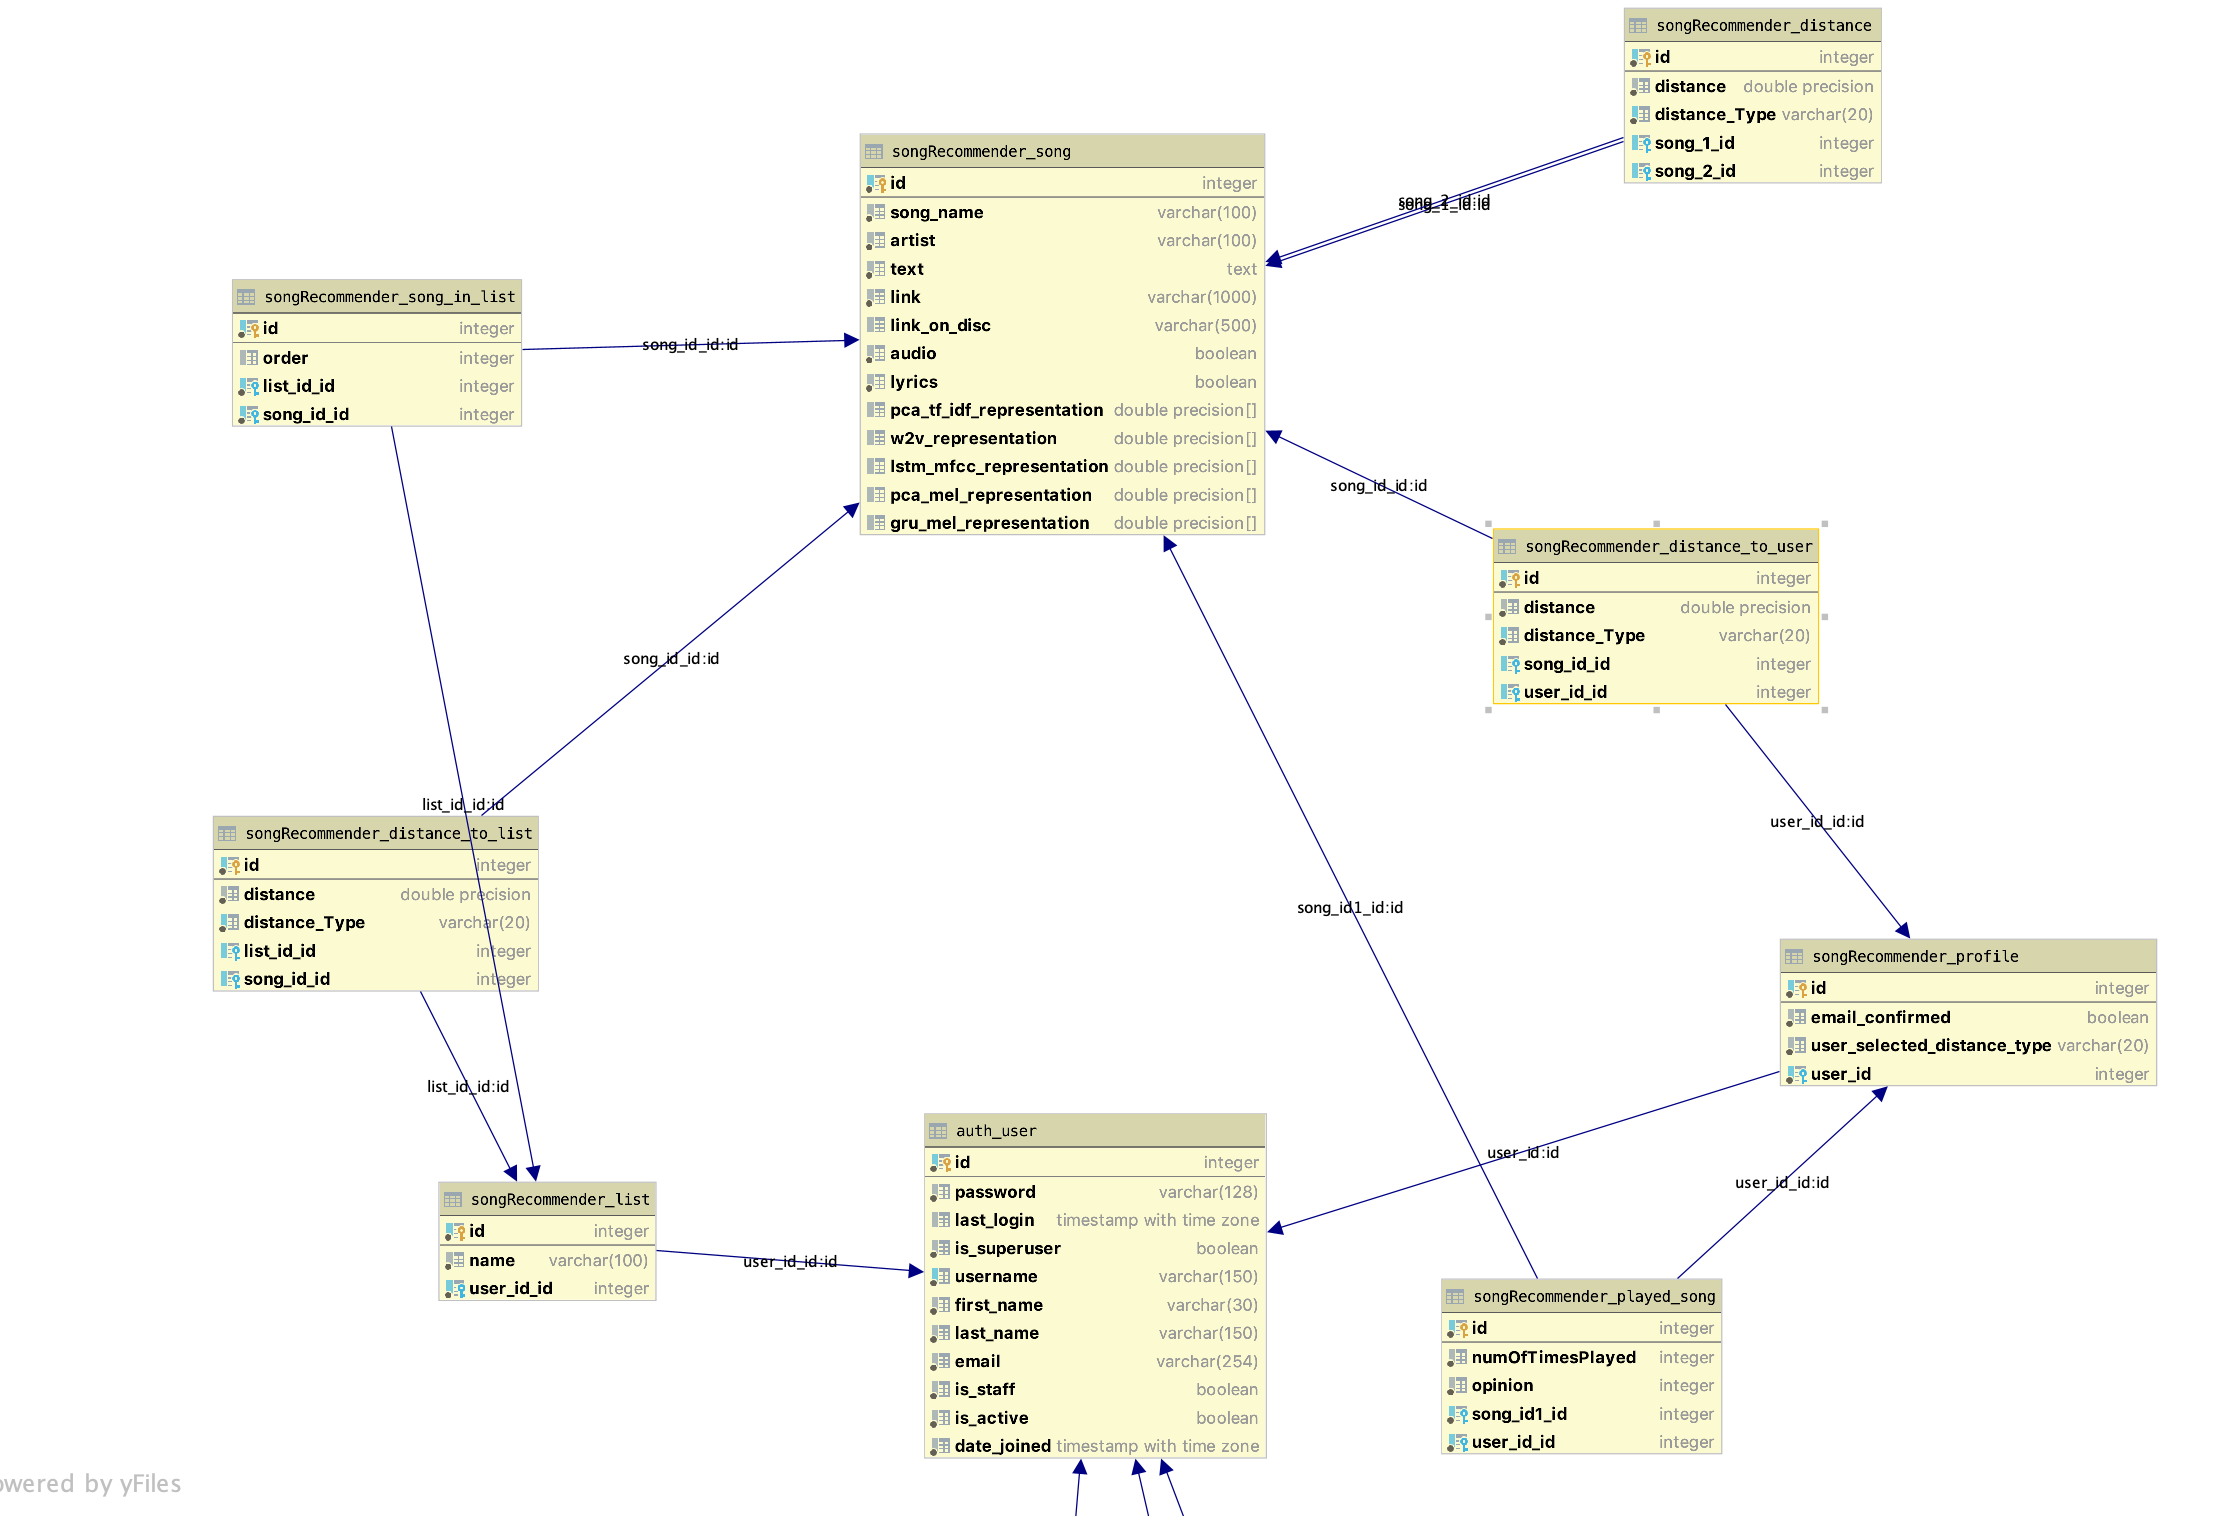
\includegraphics[width=120mm]{./img/postgres_databaze.png}
	\caption{Diagram of the applications database}
	\label{fig:diagram}
\end{figure}
The database is structured as Figure \ref{fig:diagram} illustrates. Build-in Django tables are omitted for clarity.

\subsubsection{Views}
Views handle the requests users send. Each request from some HTML page is processed by a function from \texttt{views.py}. It takes it request's parameters, calls a functions from the "logic" part of the application if necessary, collects the context for the next HTML page based on that and displays that page to the user. 

There are two main kinds of views in this application. First are build-in \textit{class-based views} which are structured around a model class from \texttt{models.py}. For exapmle the \texttt{SongDetailView} displaying a detail page of a song is a class-based view structured around the \texttt{Song}. The second are \textit{function-based views} which are not tied to a model. In the application, these are used for example for handling liking and disliking songs. 

We used both kinds of views as we could make use of the abstraction and code simplification \textit{class-based views} offer for most of the pages that revolved around models. The \textit{function based views} on the other hand provided a more flexible choice for more operational views, not only liking and disliking songs, but also changing the distance metrics etc. 

\subsubsection{Server}\label{sssec:server}

All the logic of the application is running on the server. Most expensive tasks are sent to Celery to be handled asynchronously so users do not have to wait. 
The expensive tasks are those that include calculating and recalculating song similarities. They can be triggered by four main events:

First demanding event is adding a new song. The song's mp3 is downloaded from the link the user provides, then the 15 second audio excerpt is created and turned into a mel-spectrogram and MFCC which are then input for corresponding audio method models. The songs lyrics are stripped of punctuation characters and prepared as input for the lyrics methods. After obtaining the various encodings of the newly added song, the application then calculates and stores the similarity of this song to all the other songs that are already in the database for each implemented method separately.

Afterwards, the similarity of the song to other users and to all the lists in the database is calculated and stored. Again, for each of the implemented methods. Adding a song takes about 15 seconds if there are no other songs in the database there is 1 user, 1 list and the five similarity methods we chose in Section \ref{ssec:measure_implementation} are implemented. It takes about 555 seconds if the full song dataset is loaded into the database and there is 1 user with 1 list and the same 5 methods are implemented. 

Secondly, the user can play a song for the first time. The overall recommendations are based on the songs the user has played so it is necessary recalculate similarities of all songs to the user when adding something to his \textit{played songs}.

The third event is adding a song to a list. In that case, the similarities of all songs to this list are recalculated. 

And the fourth event is liking or disliking a song, which results in recalculating similarities of all songs to the user. 

These are quite time consuming tasks especially with a growing song, list and user counts with the addition of a song being by far the most complex one. 

\subsubsection{Client}
The client only receives pre-computed HTML5 pages with some CSS for nicer design. We used the Bootstrap\footnote{https://getbootstrap.com} library which provides nice page layouts even on smaller screens and phone screens. There is no computation on the client side.

\subsection{Similarity measure implementation}\label{ssec:measure_implementation}

We did not chose methods for the application in \ref{chap:experiments} because in order to implement them, we cannot look only at their performance but also at their computational properties --- the time and space complexities. 

\subsubsection{Time and space complexity}

There are four main events described in \ref{sssec:server} that trigger the similarity calculations and recalculations in the application. However, only the duration of an addition of a new song into the database is dependant on the length of the vector representation. All the other events only use similarities already stored in the database and are represented by a single floating point number.

When a new song is added, it is transformed into the respective vector-encoding for each implemented method. Afterwards its similarity to all the songs inside the database has to be calculated. This step is the one which takes significantly longer for longer vector representations. 

A \textit{for cycle} over all songs in the database is inefficient for Python. Therefore, we take advantage of the \texttt{pairwise.metrics.cosine\_similarity} method from Python's \texttt{sklearn} package. It is the same function as we used for calculating $D_m$ matrices for evaluation. 
We insert the new vector as the first parameter and all the vector representations in the database as the second parameter of this method. The similarities are calculated for each implemented method. Because the server has limited RAM and because we do not want to limit the number of songs inside our database, we split the songs in the database into chunks and the similarities are calculated for one chunk, then saved and then the next chunk is processed. This helps us avoid a memory error even with a growing song count.

The chunk-size differs for different methods. With an increasing chunk-size the similarity calculations are faster so we made as big as possible. The size it is smaller for longer vectors and shorter for longer vectors as it is there merely to avoid a memory error and more short vectors fit into memory at once. 

The reason we care about how fast the calculations are is not really to make the next page load faster as the user does not have to wait in any case because of the asynchronous task queue. We however want our application to be responsive and recommend relevant songs as soon as possible. \\

The biggest issue with space complexity for methods is the size of their trained model. The models are needed when a new song is added to create the respective song-representation for the implemented methods. To avoid re-loading the models every time a new song is added, they are loaded into memory once at the beginning when the server starts. For some methods, the models are quite small (tens to hundreds of kilobytes) but for some, their size goes up to Gigabytes.

This poses a problem. It takes time to load big models which is the smaller issue as it happens only once in theory. However, some of them are as big as the RAM of the server so he has to put them aside while performing other tasks, which makes predictions much slower.

\subsubsection{Method selection}\label{ssec:method_selection}

With keeping the above in mind, let's look at Table \ref{table:time_space_complexities} and Figure \ref{fig:threshold_method_comparison}. We put our final choices together based on these values but there is also a third thing to consider. We are setting a higher priority on lyric based methods as they are more unique and their recommendations maybe a bit more interesting for the user. We also take the diversity of our methods into account as we want to offer an insight on how recommendtaions for various methods with various inputs look like. \\
First we rule out the method that seem to perform badly, are ranked last in most categories. It is SOM\_W2V, GRU\_Spec\_5712, LSTM\_Spec\_5712, and LSTM\_mel, and PCA\_spec\_320. \\
We also will not implement the GRU\_spec\_20400 and LSTM\_spec\_20400 and Tf-idf, raw mel-spectrograms and MFCCs because of the length of their vectors. The PCA\_spec\_1106 and PCA\_spec\_5712 disqualify because of the size of their models. \\
This leaves us with six options --- the W2V, PCA\_Tf-idf, PCA\_mel\_320,GRU\_mel, LSTM\_MFCC and the GRU\_MFCC. As we can see, none of these has spectrograms as input so we will not use any spectrogram method. Out of these, the worst one is W2V, however, it is a lyric method and it is very different from all other methods, so we decided to implement it. We left out the GRU\_MFCC as we still have have the LSTM\_MFCC network methods with the same input and GRU\_MFCC is the second worst after W2V. We could keep all the methods we did not rule out but we want to reduce the number of methods because the distance calculations are not calculated in parallel (although they could be) but one after another. More methods are therefore more complex. \\
Let's recapitulate our method choices:
\begin{itemize}
    \item \textbf{PCA\_Tf-idf} is a lyrics-based method and also the best method we presented with reasonable vector length.
    \item \textbf{W2V} is also a lyrics-based method, it is the worst from the ones we decided to implement but it has short vectors and a small model and helps with method diversity.
    \item \textbf{PCA\_mel\_320} is the first audio based method. It appears to be good in the average rank of a song, however, that is not so important for recommendation. Its overall results are average and its time and space complexities very convenient.
    \item \textbf{GRU\_mel} is also deep neural network method which performed best between neural networks.
    \item \textbf{LSTM\_MFCC} is another deep neural network method which has two components we have not used in any of our implemented methods, the LSTM layers in its architecture and takes the MFCCs as input. It is unique with good results relative to other methods. 
\end{itemize}

\begin{table}[h]
\centering
\renewcommand{\arraystretch}{1.5}
\begin{tabu} to 1\textwidth {| c || X[c] | X[c] | }
 \hline
 \textbf{method} & \textbf{vector length} & \textbf{model size in KB} \\
 \hline
 raw mel-spectrograms & 130,560 & no model \\
 \hline 
 raw MFCCs & 82,688 & no model \\
 \hline
 Tf-idf & 40,165 & 2,600 \\
 \hline
 PCA on Tf-idf & 4,457 & 1,430,000  \\
 \hline
 W2V & 300 & 251,100 \\
 \hline
 SOM\_W2V & 2 & 358,792 \\
 \hline
 PCA\_spec\_1106 & 1,106 & 7,980,000 \\
 \hline
 PCA\_spec\_320 & 320 & 2,320,000\\
 \hline
 PCA\_mel\_5715 & 5,715 & 5,970,000\\
 \hline
 PCA\_mel\_320 & 320 & 336,300 \\
 \hline
 GRU\_spec\_20400 & 20,400 & 67,000 \\
 \hline
 GRU\_spec\_5712 & 5,712 & 59,000 \\
 \hline
 LSTM\_spec\_20400 & 20,400 & 3700 \\
 \hline
 LSTM\_spec\_5712 & 5,712 & 1003 \\
 \hline
 GRU\_mel & 5,712 & 146 \\
 \hline
 LSTM\_mel & 5,712 & 185 \\
 \hline
 GRU\_MFCC & 5,168 & 48 \\
 \hline
 LSTM\_MFCC & 5,168 & 471 \\
 \hline
 \end{tabu} \\
\caption{The vector length and model size for different methods}
\label{table:time_space_complexities}
\end{table}

\subsubsection{Recommendation calculation}\label{ssec:recom_calcs}

The similarity of two songs is calculated using the cosine similarity with threshold $cos\_sim_t$ as described in Subsection
\ref{ssec:evaluation_measures}. The similarity of a song to a user is an addition of similarities. To be specific, the similarity of a song $s_i$ to a user $U$ is calculated as: $$ \sum_{k=0}^{k=n} c*cos\_sim_t(s_i, s_k) $$  where $ i \neq k $ and $ s_k $ is a song the user's played songs and $n$ is the number of songs the user has played and $c$ is a constant which is either 1 when the song $s_k$ was played or 2 when $s_k$ was also liked. 
The similarity of a song $s_i$ to a list $L$ is calculated as:
$$ \sum_{l=0}^{l=m} c*cos\_sim_t(s_i, s_l) $$ 
where $ i \neq l $, $m$ is the number of songs in list $L$, $s_l$ is a song from list L and $c$ is the same constant as before.

The displayed recommendations do not include songs the user has already played. It is also possible to see always only the top 10 recommendations, overall and for a each list. For the detail page of a song there is an audio area where it is possible to play the song and its 10 most similar song. There is also a possibility to like it or dislike it.  

\subsection{Base data import}

To provide songs to users of the application from the beginning, we uploaded the data from the SD dataset and the data we acquired during experimentation to the database. This made them available in the application from the moment of its launching. 

The methods that were used to transfer the data into the database are in the \texttt{data/load\_distances.py} module. The songs from SD with corresponding titles, artists, lyrics, YouTube links, and paths to .mp3 files in the file system were stored using the \texttt{load\_song\_to\_database} as instances of the class \texttt{Song}. Afterwards, we added all five vector representations of the five implemented methods to each of the 16,594 \texttt{Song} instances using the \texttt{load\_all\_representations} method. The representations were extracted from the $R_m$ matrices. Finally, we called the \texttt{load\_all\_distances} method to create instances of the \texttt{Distance} class for the similarities from $D_m$ matrices that were above the 0.03\% threshold meaning, there are about 829,700 instances of \texttt{Distance} for each of the five implemented similarity methods.

\section{Configuration options}\label{sec:configurations}

In this section we will describe the configuration options the application provides. There are some options that influence recommendation as well as options to change the server settings. All of the configurations are in the module \texttt{setting.py}

\subsection{Similarity method configurations}
The things that can be set for similarity methods are the thresholds. Right now, the threshold values correspond the to keeping 827,900 biggest similarities for each similarity method, meaning, there are about 50*16594 instances of \texttt{Distance} stored in the database for each of the implemented methods. Changing the threshold does not influence the songs that are already in the database. Nevertheless, when a new song is added, potentially more distances will be created, when the threshold is lowered, or less, when its raised. \\
Another thing that can be configured in the \texttt{setting.py} module is the default similarity method that is assigned to a new user account. The user can then change it once he is logged in.

\subsection{Email}
There is a boolean variable called \texttt{EMAIL\_DISABLED} which is set on True by default as there is no email service set up with our application, however if a email service and a domain is provided, it is only necessary to change the \texttt{EMAIL\_DISABLED} variable to False and delete the \texttt{EMAIL\_BACKEND} and replace it with an email service configuration. If the variable is set to False without configuring an email service, the email is printed to the console and the user has no way of authenticating his account.

\subsection{Server}

The application has not been completely deployed. It runs on \url{http://acheron.ms.mff.cuni.cz:42009/index/} in debug mode. To actually deploy the application, it is necessary go to \texttt{settings.py} and change the \texttt{Debug} variable to \texttt{False}. Then it is necessary to collect all static files (including all the mp3 files) and tell Django where they are as it stops handling static files itself without the debug mode on. It is also necessary to choose some wsgi, for example \texttt{gunicorn}\footnote{https://gunicorn.org} with \texttt{nginx}\footnote{https://nginx.org/en/} or \texttt{apache}\footnote{https://httpd.apache.org} as web servers.









\chapter*{Conclusion}
The goal of this this thesis was to test and implement multiple content-based recommendation techniques. On the way, we dealt with many various tasks from building a web application (which has it perks itself for example dealing with the database, python package compatibility, server configuration, celery configuration, ...) to extracting music audios, handling GPU drivers, building neural networks etc. At the end, we can say that we successfully introduced a running web application with recommendation methods that provide users with relevant recommendations (compared to for example random recommendations). \\
Our most successful method -- the PCA\_Tf-idf method -- is lyrics based which was not expected. From that we can conclude that creating lyrics-based recommendation applications is not unreasonable. Audio methods also proved to yield good results.

\subsection{Future work}
\subsubsection{Recommendation methods}
Further study of lyric-based method is one way to go in future work. We could use for example the Tf-idf vectors not only as input for the PCA or SOM but also for other types of neural networks. They might not be suited for RNN networks as there is no kind of sequential information stored in the Tf-idf vector but it would be interesting to try different architectures. \\
As we tested our audio methods, some proved to be more perspective than others. Mel-spectrograms and MFCCs seem to be a better input for similarity methods than raw spectrograms. Also the PCA showed to have great potential with both lyrics and audio based methods so further research into this seems to be a good idea. \\
When it comes to neural networks, networks with the "GRU" layers seem to perform better than "LSTM" layers. Also various different architectures can be tested. Using other types of neural networks than RNNs seems as a reasonable thing to do because it appears that reducing only the number of features is limiting for these networks, as the PCA which reduced the features and the samples might have benefited mainly from that. \\
\subsubsection{Web application}
The web application can be further extended in multiple ways. One thing would be creating a system, where the users could rate the recommendations so we would have feedback about method performance not only from the evaluation we did in this thesis but also from real time users. \\
Also more advanced recommendation metrics could be applied in the web application. We could keep track on the users lastly played songs or take into account how many times he played a song and then use this in the final similarity calculation. For example have something like \textit{The most similar songs to the last 10 you played} or \textit{The most similar songs to your 10 most played songs} etc. \\
There is obviously also the possibility of including more similarity methods into the application, which however now involves a non-trivial amount of changes to the source code. So maybe also a simplification and better design pattern for the "logic" of the application could be a step to take in the future. \\
Then there are some application features that could be implemented which follow the design of traditional music-applications. This includes playing whole playlists or creating an endless playlist from the recommendations as well as adding videos and tags to songs and allow searching based on genres etc. \\

\addcontentsline{toc}{chapter}{Conclusion}


%%% Bibliography
%%% Bibliography (literature used as a source)
%%%
%%% We employ bibTeX to construct the bibliography. It processes
%%% citations in the text (e.g., the \cite{...} macro) and looks up
%%% relevant entries in the bibliography.bib file.
%%%
%%% The \bibliographystyle command selects, which style will be used
%%% for references from the text. The argument in curly brackets is
%%% the name of the corresponding style file (*.bst). Both styles
%%% mentioned in this template are included in LaTeX distributions.

%b\bibliographystyle{plainnat}    %% Author (year)
\bibliographystyle{unsrt}     %% [number]

\renewcommand{\bibname}{Bibliography}

%%% Generate the bibliography. Beware that if you cited no works,
%%% the empty list will be omitted completely.

\bibliography{bibliography}

%%% If case you prefer to write the bibliography manually (without bibTeX),
%%% you can use the following. Please follow the ISO 690 standard and
%%% citation conventions of your field of research.

% \begin{thebibliography}{99}
%
% \bibitem{lamport94}
%   {\sc Lamport,} Leslie.
%   \emph{\LaTeX: A Document Preparation System}.
%   2nd edition.
%   Massachusetts: Addison Wesley, 1994.
%   ISBN 0-201-52983-1.
%
% \end{thebibliography}


%%% Figures used in the thesis (consider if this is needed)
\listoffigures

%%% Tables used in the thesis (consider if this is needed)
%%% In mathematical theses, it could be better to move the list of tables to the beginning of the thesis.
\listoftables

%%% Abbreviations used in the thesis, if any, including their explanation
%%% In mathematical theses, it could be better to move the list of abbreviations to the beginning of the thesis.

%%% Attachments to the bachelor thesis, if any. Each attachment must be
%%% referred to at least once from the text of the thesis. Attachments
%%% are numbered.
%%%
%%% The printed version should preferably contain attachments, which can be
%%% read (additional tables and charts, supplementary text, examples of
%%% program output, etc.). The electronic version is more suited for attachments
%%% which will likely be used in an electronic form rather than read (program
%%% source code, data files, interactive charts, etc.). Electronic attachments
%%% should be uploaded to SIS and optionally also included in the thesis on a~CD/DVD.
%%% Allowed file formats are specified in provision of the rector no. 72/2017.
\appendix
\chapter{Attachments}

\section{First Attachment}\label{attach:first_attachment}

The zipped attachment has the following contents:
\begin{itemize}
    \item The text of the thesis in pdf format under the name \texttt{thesis\_text.pdf}
    \item A folder called \texttt{songRecommender\_project} containing the source code of the project with a \texttt{README.md} file that describes the project's directories and modules.
    \item User documentation in pdf format under the name \texttt{sr\_UserDocs.pdf}
\end{itemize}

\openright
\end{document}
